\chapter{Thực nghiệm và Đánh giá kết quả}
\label{ch:thucnghiem}

Chương này trình bày chi tiết môi trường thực nghiệm, thiết lập huấn luyện, kết quả đạt được và phân tích đánh giá cho cả hai thành phần chính: (1) Phát hiện và theo dõi phương tiện, (2) Nhận diện biển số xe.

%============================================================
% PHẦN 1: MÔI TRƯỜNG THỰC NGHIỆM
%============================================================
\section{Môi trường thực nghiệm}

\subsection{Cấu hình phần cứng}

Các thực nghiệm trong nghiên cứu này được triển khai trên hai nền tảng: đám mây Kaggle Notebooks cho huấn luyện và máy tính cục bộ cho inference.

\begin{table}[ht!]
    \centering
    \caption{Cấu hình chi tiết môi trường thực nghiệm}
    \label{tab:system_config}
    \begin{tabular}{|l|l|}
        \hline
        \textbf{Thành phần} & \textbf{Thông số kỹ thuật} \\ \hline
        \multicolumn{2}{|c|}{\textit{Huấn luyện (Kaggle Cloud)}} \\ \hline
        CPU & 4 Logical Cores \\ \hline
        RAM & 31.35 GB \\ \hline
        GPU & NVIDIA Tesla P100-PCIE (16GB VRAM) \\ \hline
        Dung lượng đĩa & 19.52 GB \\ \hline
        \multicolumn{2}{|c|}{\textit{Inference (Local Machine)}} \\ \hline
        CPU & Intel Core i5-12400 \\ \hline
        RAM & 16GB DDR4 \\ \hline
        GPU & NVIDIA RTX 4060 \& RTX 2050 \\ \hline
    \end{tabular}
\end{table}

\subsection{Cấu hình phần mềm}

\begin{itemize}
    \item Ngôn ngữ lập trình: Python 3.10/3.11
    \item Nền tảng tính toán song song: CUDA 11.8/12.4
    \item Framework Deep Learning: PyTorch 2.0
    \item Ultralytics YOLOv8: Version 8.0.196
    \item PaddleOCR: Version 2.7.0
    \item OpenCV: Version 4.8.0
    \item PyQt5: Giao diện người dùng
\end{itemize}

%============================================================
% PHẦN 2: KẾT QUẢ PHÁT HIỆN PHƯƠNG TIỆN
%============================================================
\section{Kết quả huấn luyện mô hình phát hiện phương tiện}

\subsection{Thiết lập huấn luyện}

\subsubsection{Chiến lược tăng cường dữ liệu}
Hệ thống áp dụng kỹ thuật \textbf{Mosaic Augmentation} (ghép 4 ảnh ngẫu nhiên thành 1) trong quá trình huấn luyện (xem Hình \ref{fig:mosaic_aug}). Kỹ thuật này đặc biệt hiệu quả cho bài toán giao thông vì:
\begin{itemize}
    \item Giúp mô hình học được các ngữ cảnh phức tạp và các vật thể bị che khuất một phần.
    \item Cải thiện khả năng phát hiện các đối tượng nhỏ (như xe máy, xe đạp ở xa) bằng cách thay đổi tỷ lệ ảnh.
\end{itemize}

\begin{figure}[H]
    \centering
    \begin{tabular}{cc}
         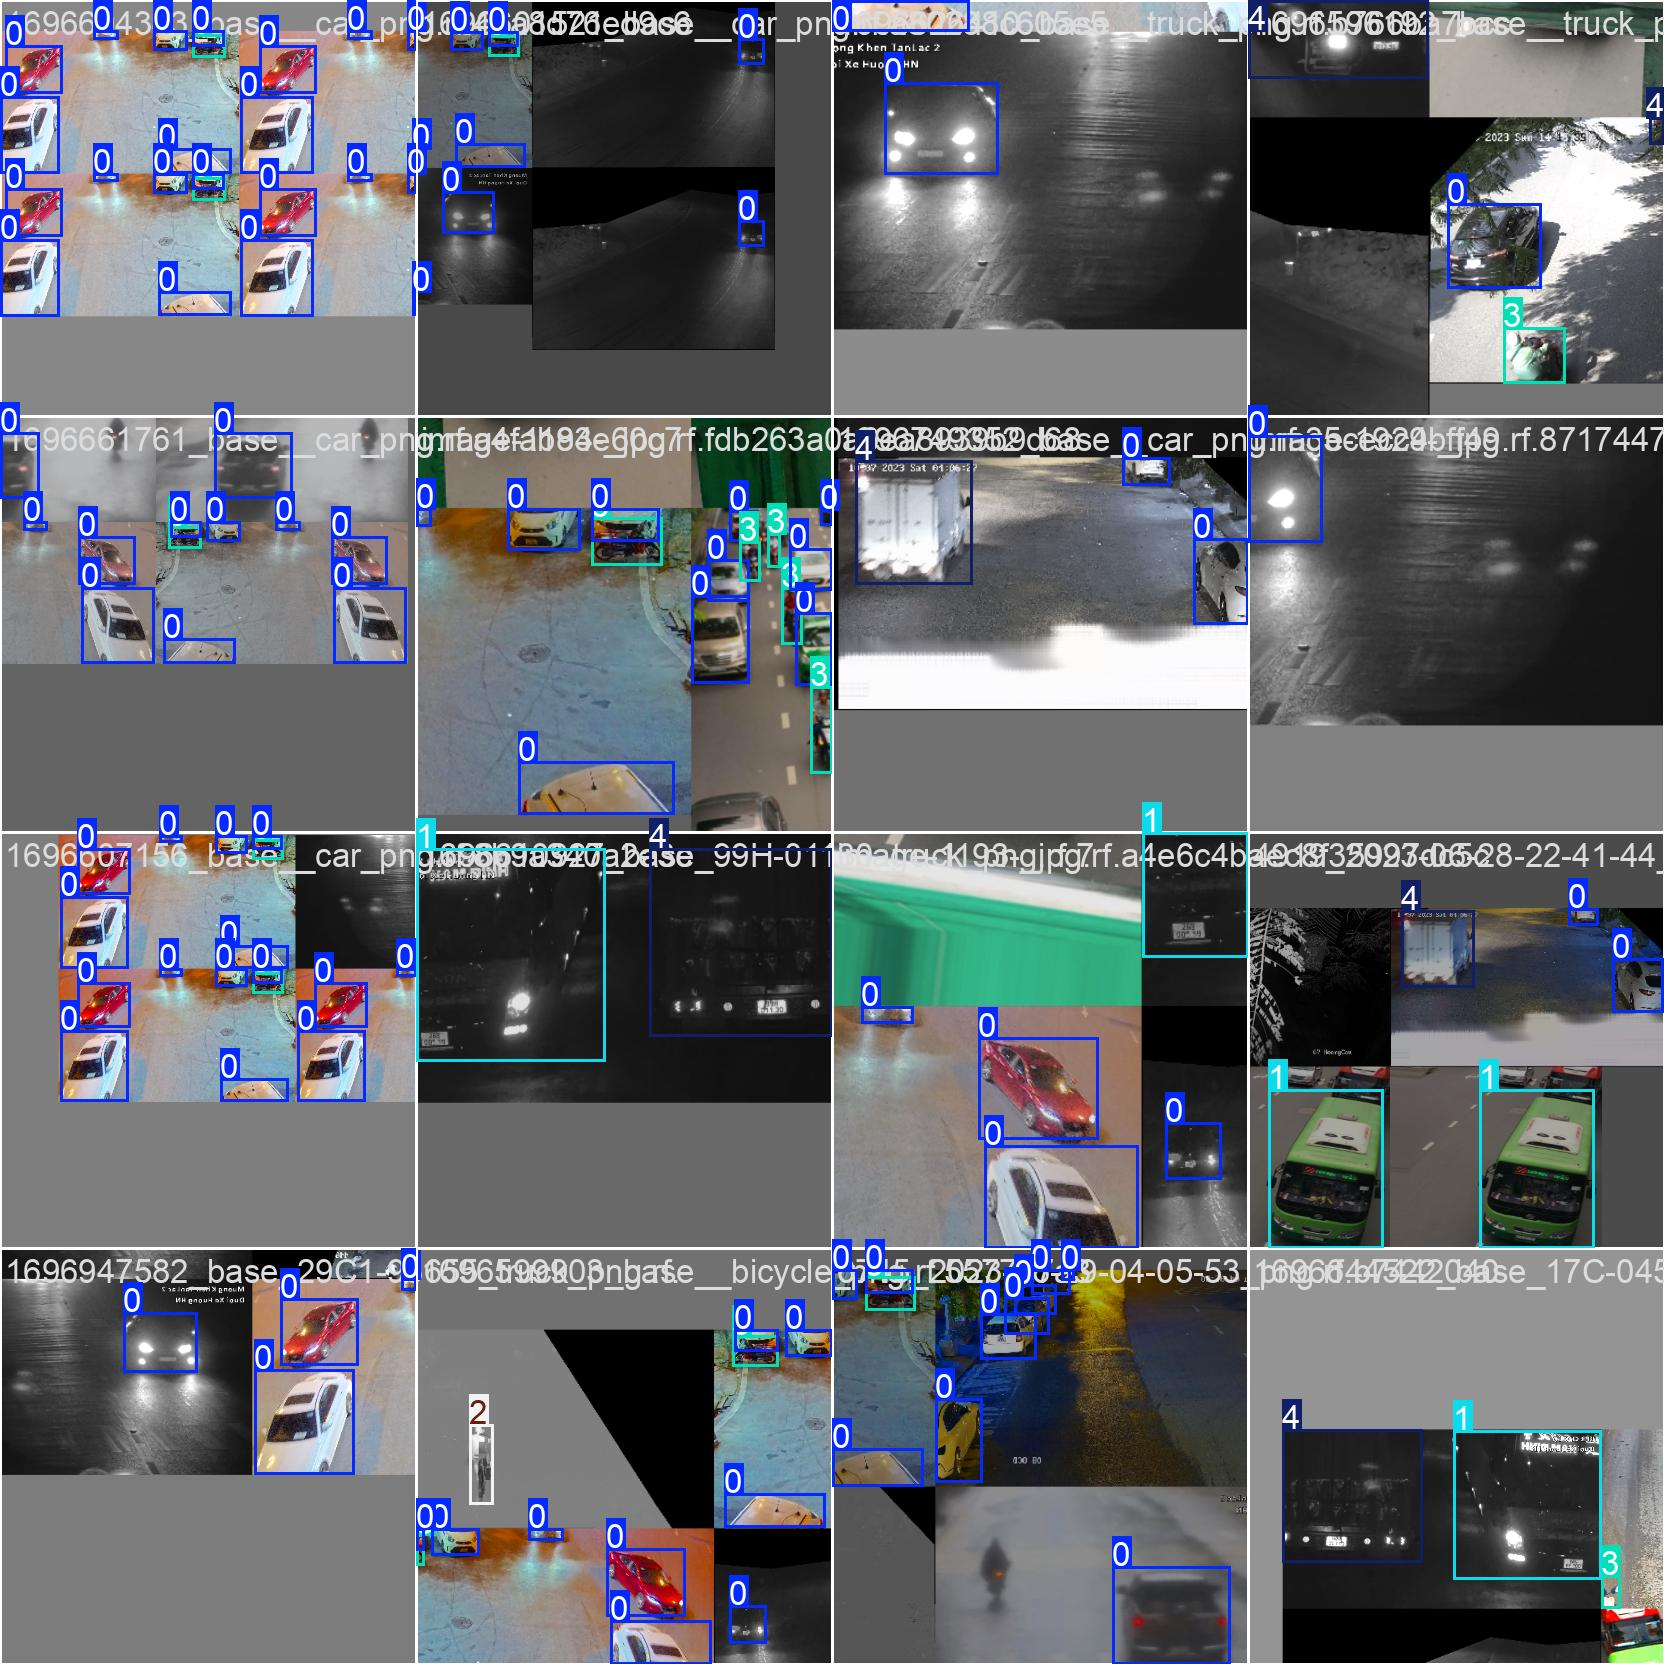
\includegraphics[width=0.45\linewidth]{Figures/train_batch0.jpg} &
         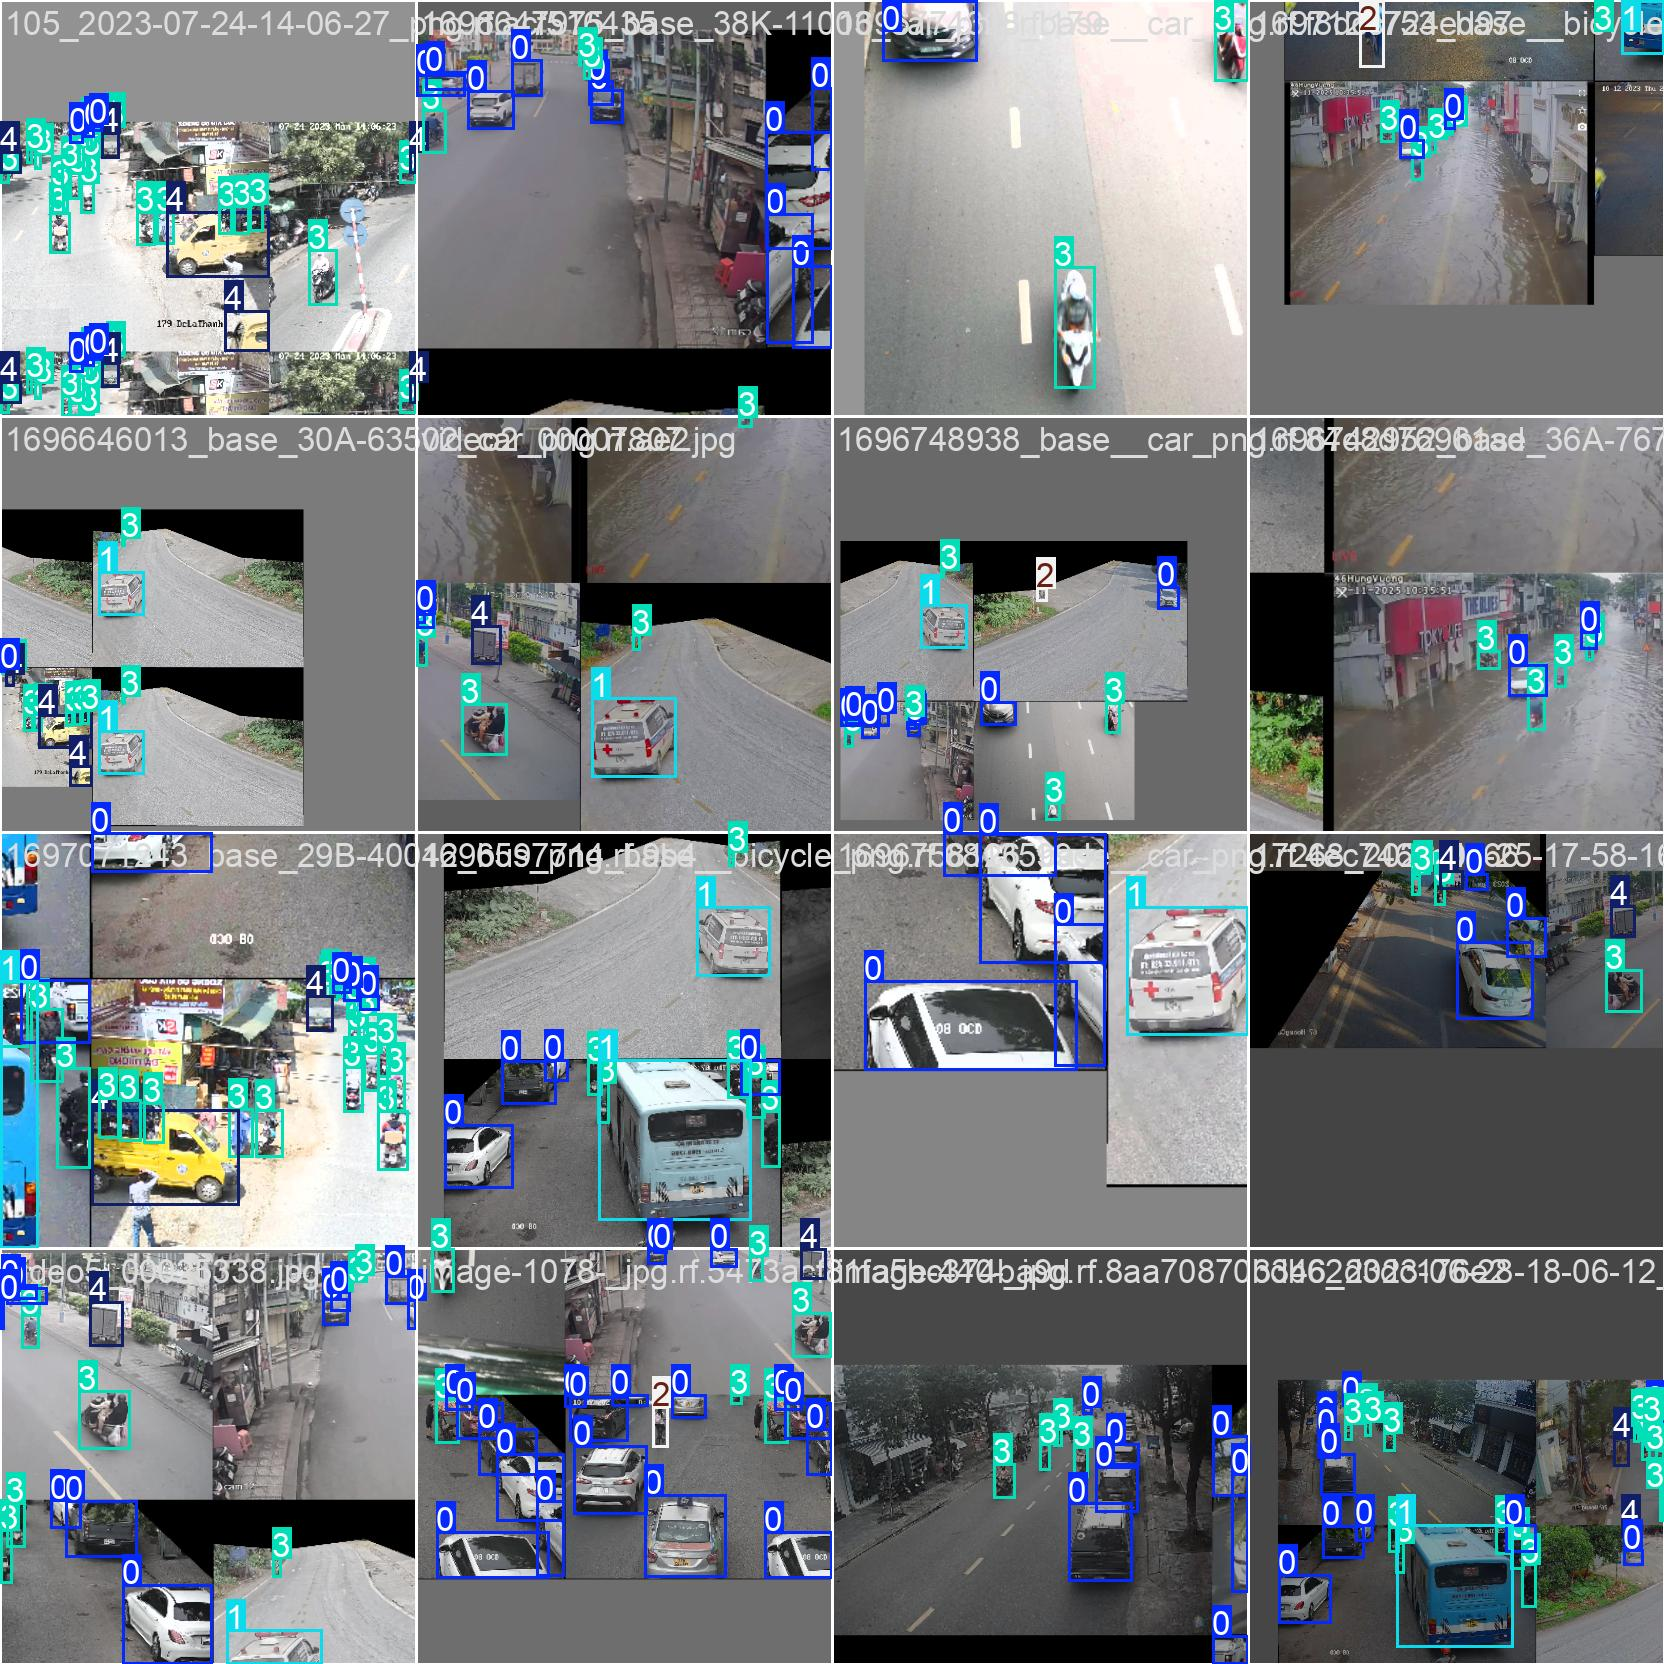
\includegraphics[width=0.45\linewidth]{Figures/train_batch1.jpg} \\
         (a) Batch 0 & (b) Batch 1
    \end{tabular}
    \caption{Dữ liệu huấn luyện sau khi áp dụng Mosaic Augmentation}
    \label{fig:mosaic_aug}
\end{figure}

\subsection{Phân tích quá trình hội tụ}
Biểu đồ \ref{fig:results_chart} thể hiện diễn biến của các hàm mất mát và chỉ số mAP qua 100 epochs.

\begin{figure}[H]
    \centering
    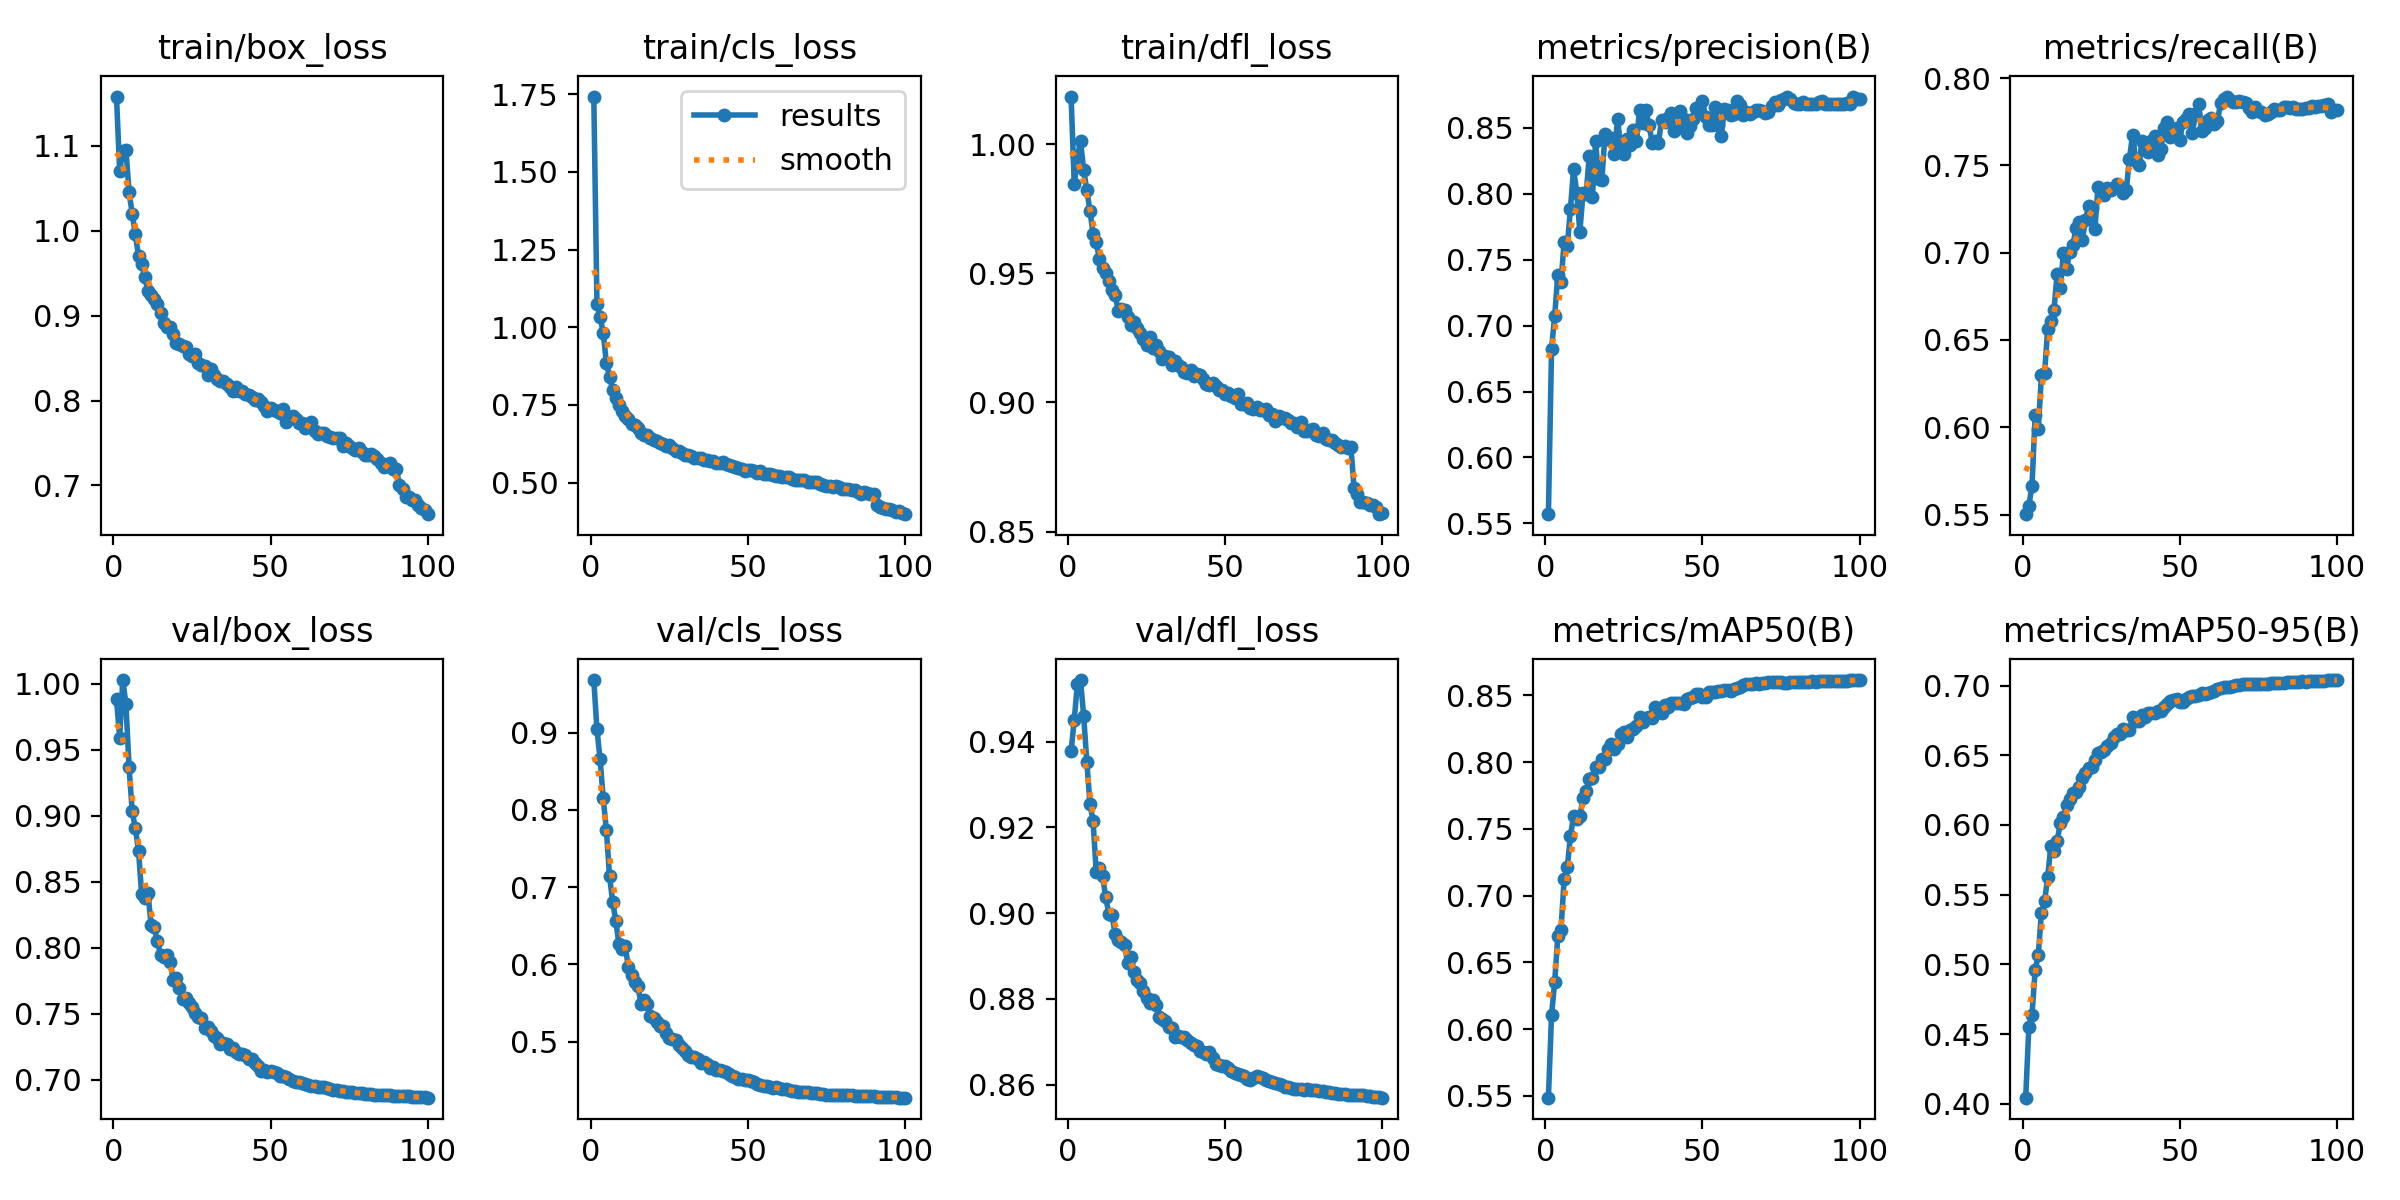
\includegraphics[width=0.95\linewidth]{Figures/results.png}
    \caption{Đồ thị Loss và mAP trong quá trình huấn luyện phát hiện phương tiện}
    \label{fig:results_chart}
\end{figure}

\textbf{Nhận xét:}
\begin{itemize}
    \item \textbf{Sự hội tụ:} Các hàm mất mát (\texttt{box\_loss}, \texttt{cls\_loss}) giảm nhanh trong 20 epoch đầu và tiếp tục giảm nhẹ, ổn định dần về phía cuối chu kỳ huấn luyện. Không xuất hiện hiện tượng \textit{overfitting} khi loss của tập validation bám sát tập train.
    \item \textbf{Hiệu năng:} Chỉ số mAP@50 tăng trưởng mạnh và đạt trạng thái bão hòa từ epoch thứ 80 trở đi, cho thấy việc dừng huấn luyện tại 100 epoch là hợp lý.
\end{itemize}

\subsection{Kết quả định lượng}
Tại epoch tốt nhất (Epoch 99), mô hình đạt được các chỉ số hiệu năng ấn tượng trên tập Validation:

\begin{table}[H]
\centering
\caption{Kết quả đánh giá hiệu năng mô hình YOLOv8n phát hiện phương tiện}
\label{tab:final_metrics_vehicle}
\begin{tabular}{|l|c|c|c|c|}
\hline
\textbf{Chỉ số} & \textbf{Precision(P)} & \textbf{Recall(R)} & \textbf{mAP@50} & \textbf{mAP@50:95} \\ \hline
\textbf{Giá trị} & \textbf{0.872} & \textbf{0.781} & \textbf{0.861} & \textbf{0.704} \\ \hline
\end{tabular}
\end{table}

\subsubsection{Kết quả chi tiết theo từng lớp}
Phân tích chi tiết theo từng lớp đối tượng:

\begin{table}[H]
\centering
\caption{Kết quả mAP@50 theo từng lớp phương tiện}
\label{tab:class_metrics}
\begin{tabular}{|l|c|c|c|}
\hline
\textbf{Lớp} & \textbf{mAP@50} & \textbf{Precision} & \textbf{Recall} \\ \hline
Ô tô (o to) & 0.922 & 0.91 & 0.85 \\ \hline
Xe buýt (xe bus) & 0.897 & 0.88 & 0.80 \\ \hline
Xe máy (xe may) & 0.872 & 0.85 & 0.79 \\ \hline
Xe tải (xe tai) & 0.832 & 0.84 & 0.75 \\ \hline
Xe đạp (xe dap) & 0.782 & 0.78 & 0.72 \\ \hline
\end{tabular}
\end{table}

\begin{itemize}
    \item Lớp \textbf{"Ô tô" (o to)} đạt hiệu quả cao nhất với \textbf{mAP@50 = 0.922}.
    \item Lớp \textbf{"Xe buýt" (xe bus)} đạt \textbf{0.897} và \textbf{"Xe máy" (xe may)} đạt \textbf{0.872}.
    \item Lớp \textbf{"Xe đạp" (xe dap)} có hiệu năng thấp nhất (\textbf{0.782}), phản ánh độ khó trong việc phân biệt loại phương tiện thô sơ này.
\end{itemize}

\subsection{Phân tích lỗi qua ma trận nhầm lẫn}
Dựa trên ma trận nhầm lẫn chuẩn hóa (Hình \ref{fig:conf_matrix}), ta nhận diện được các điểm yếu cụ thể của mô hình:

\begin{figure}[H]
    \centering
    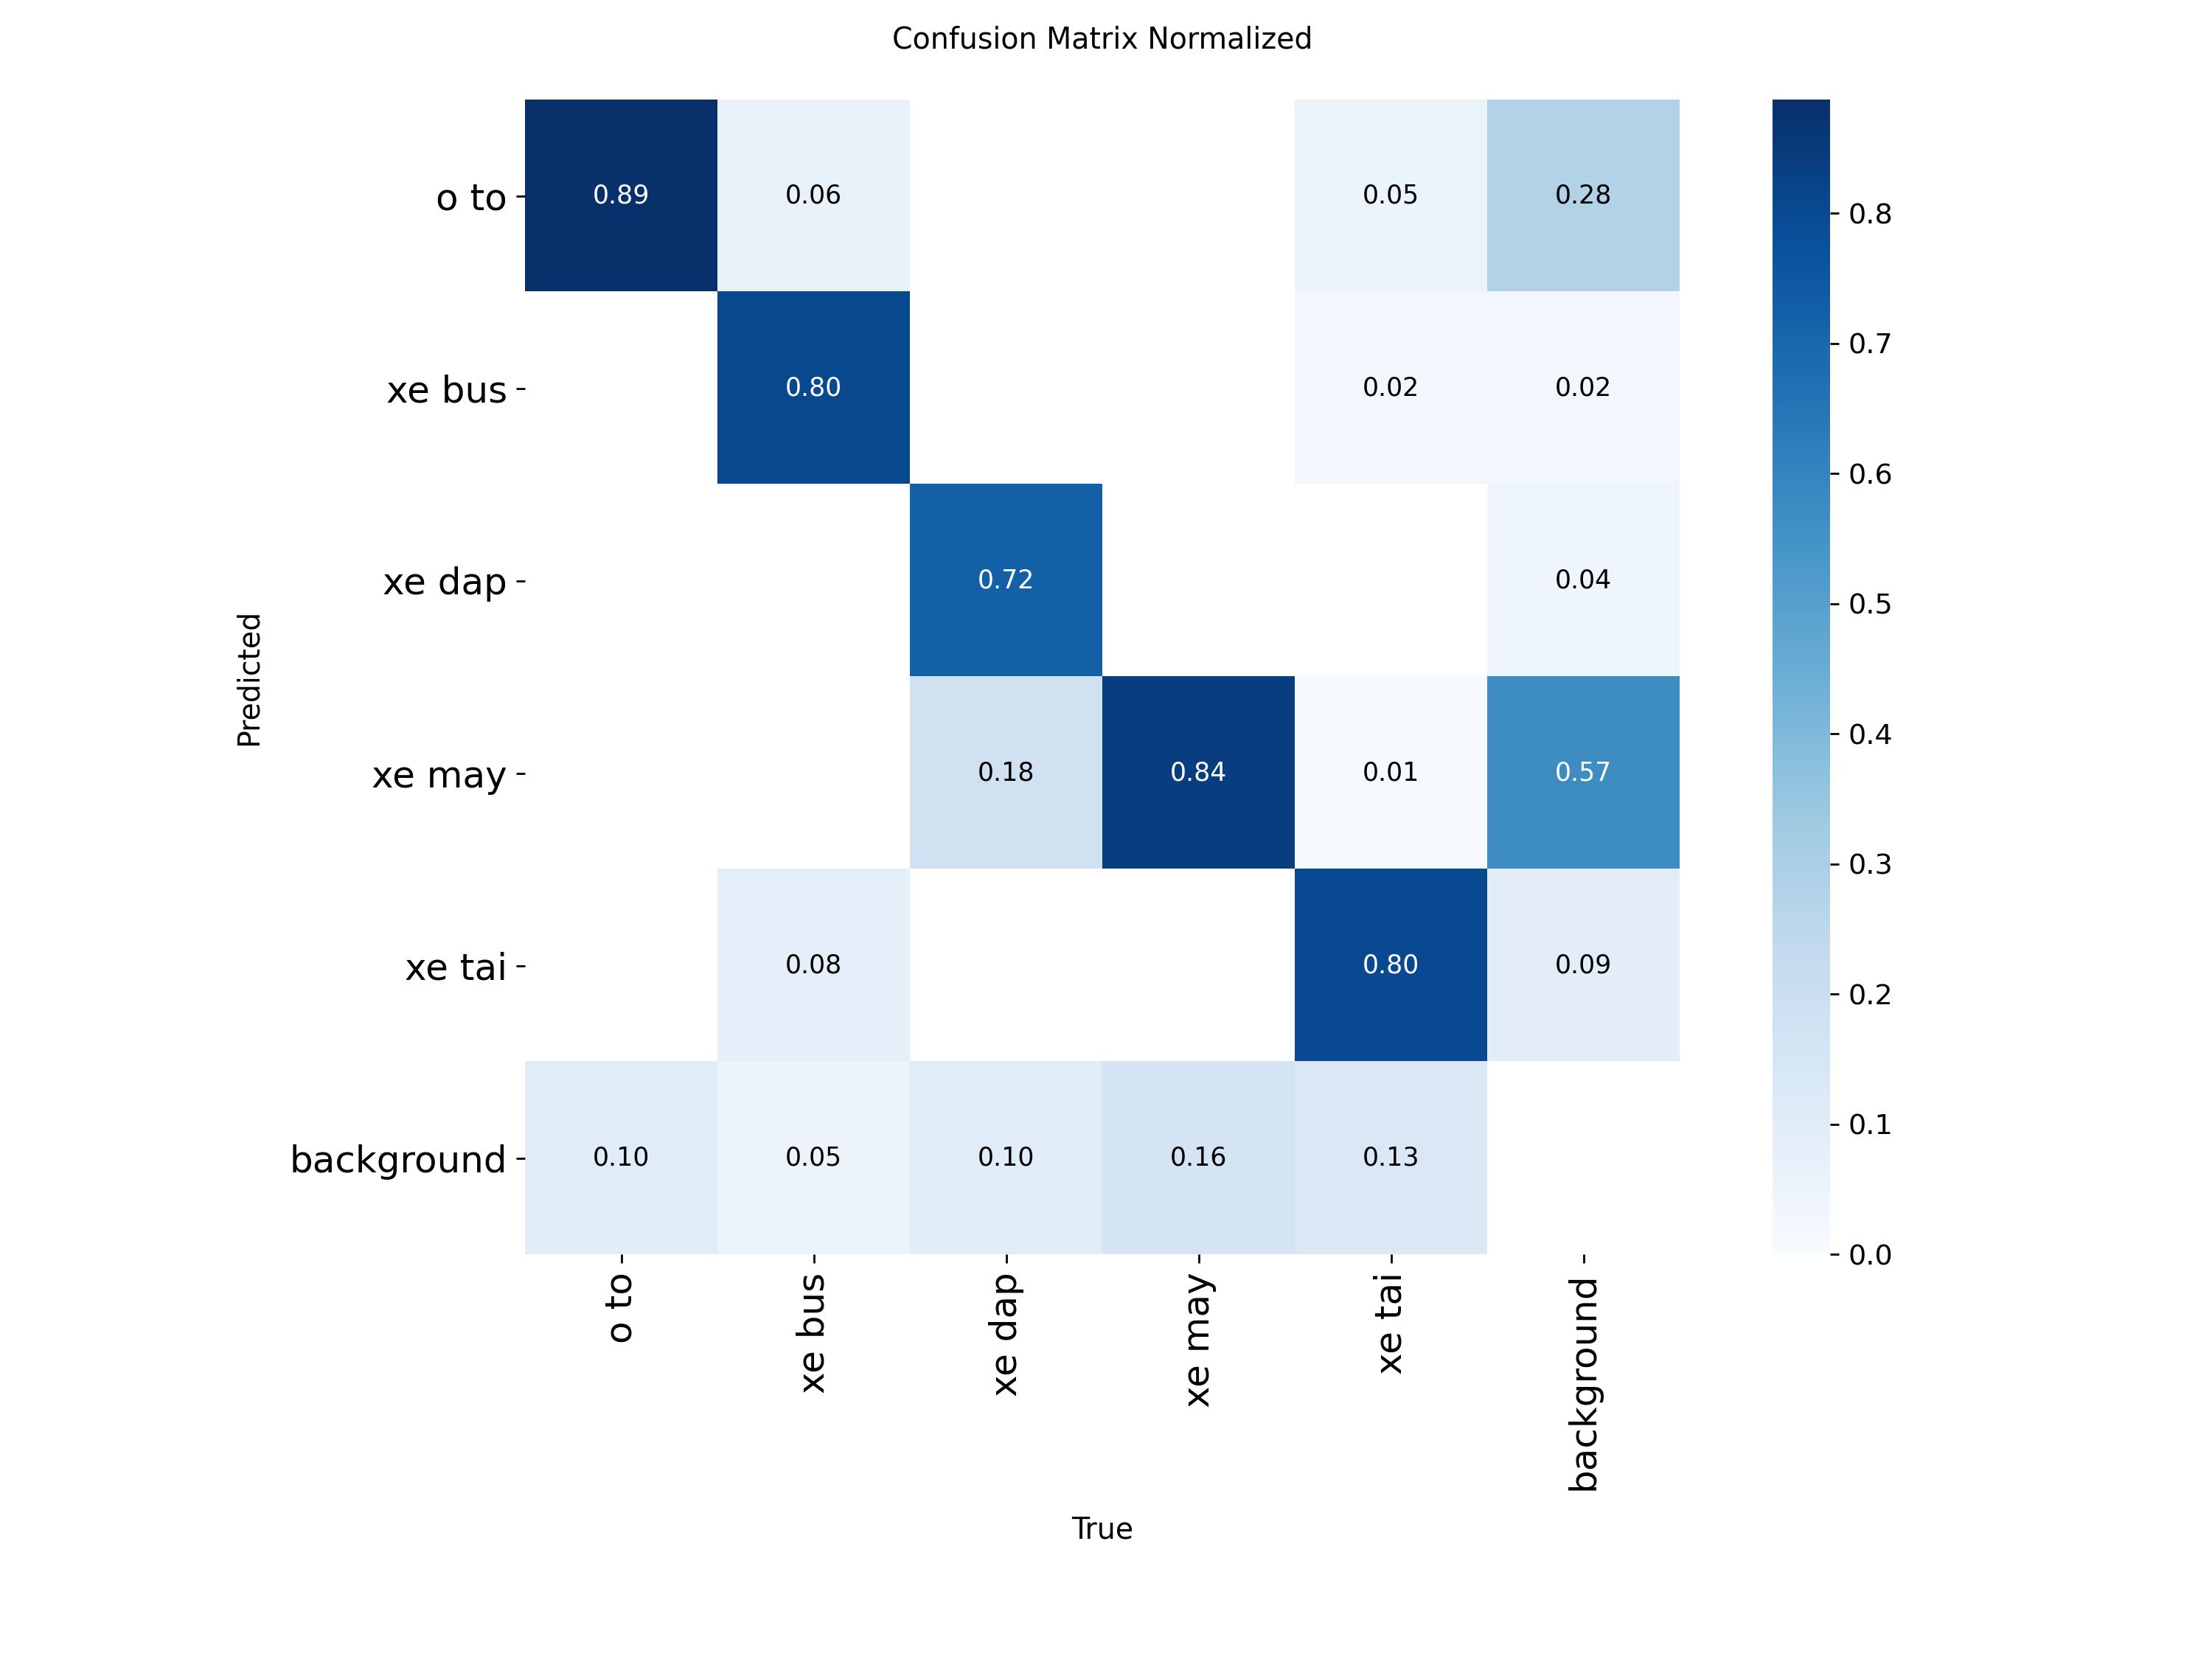
\includegraphics[width=0.7\linewidth]{Figures/confusion_matrix_normalized.png}
    \caption{Ma trận nhầm lẫn chuẩn hóa (Normalized Confusion Matrix)}
    \label{fig:conf_matrix}
\end{figure}

\begin{itemize}
    \item \textbf{Nhầm lẫn nghiêm trọng nhất:} Có tới \textbf{18\%} số lượng \textit{Xe đạp} bị mô hình dự đoán nhầm thành \textit{Xe máy}. Nguyên nhân do hình dáng cấu trúc tương đồng (2 bánh, người ngồi trên) và kích thước nhỏ khi nhìn từ xa.
    \item \textbf{Bỏ sót đối tượng (Background FN):} Khoảng \textbf{16\%} xe máy bị bỏ sót (nhận diện là background), thường rơi vào các trường hợp xe bị che khuất hoặc trong điều kiện ánh sáng yếu (ban đêm).
    \item \textbf{Độ chính xác cao:} Ô tô và Xe buýt rất ít khi bị nhầm lẫn với các lớp khác (tỷ lệ chính xác lần lượt là 89\% và 80\%).
\end{itemize}

\subsection{Đánh giá định tính}


Mô hình thể hiện khả năng bao quát tốt trong điều kiện giao thông hỗn loạn. Các bounding box bám sát đối tượng. Đặc biệt, hệ thống xử lý tốt các trường hợp \textbf{xe máy đi thành cụm đông đúc} mà không bị gộp box (nhờ thuật toán NMS hoạt động hiệu quả). Tuy nhiên, vẫn còn một số trường hợp xe ở quá xa hoặc tối bị bỏ sót như phân tích ở trên.

\subsection{Đường cong Precision-Recall}
Đường cong PR (Hình \ref{fig:vehicle_pr_curve}) cho thấy mô hình đạt được sự cân bằng tốt giữa Precision và Recall trên tất cả các lớp phương tiện.

\begin{figure}[H]
    \centering
    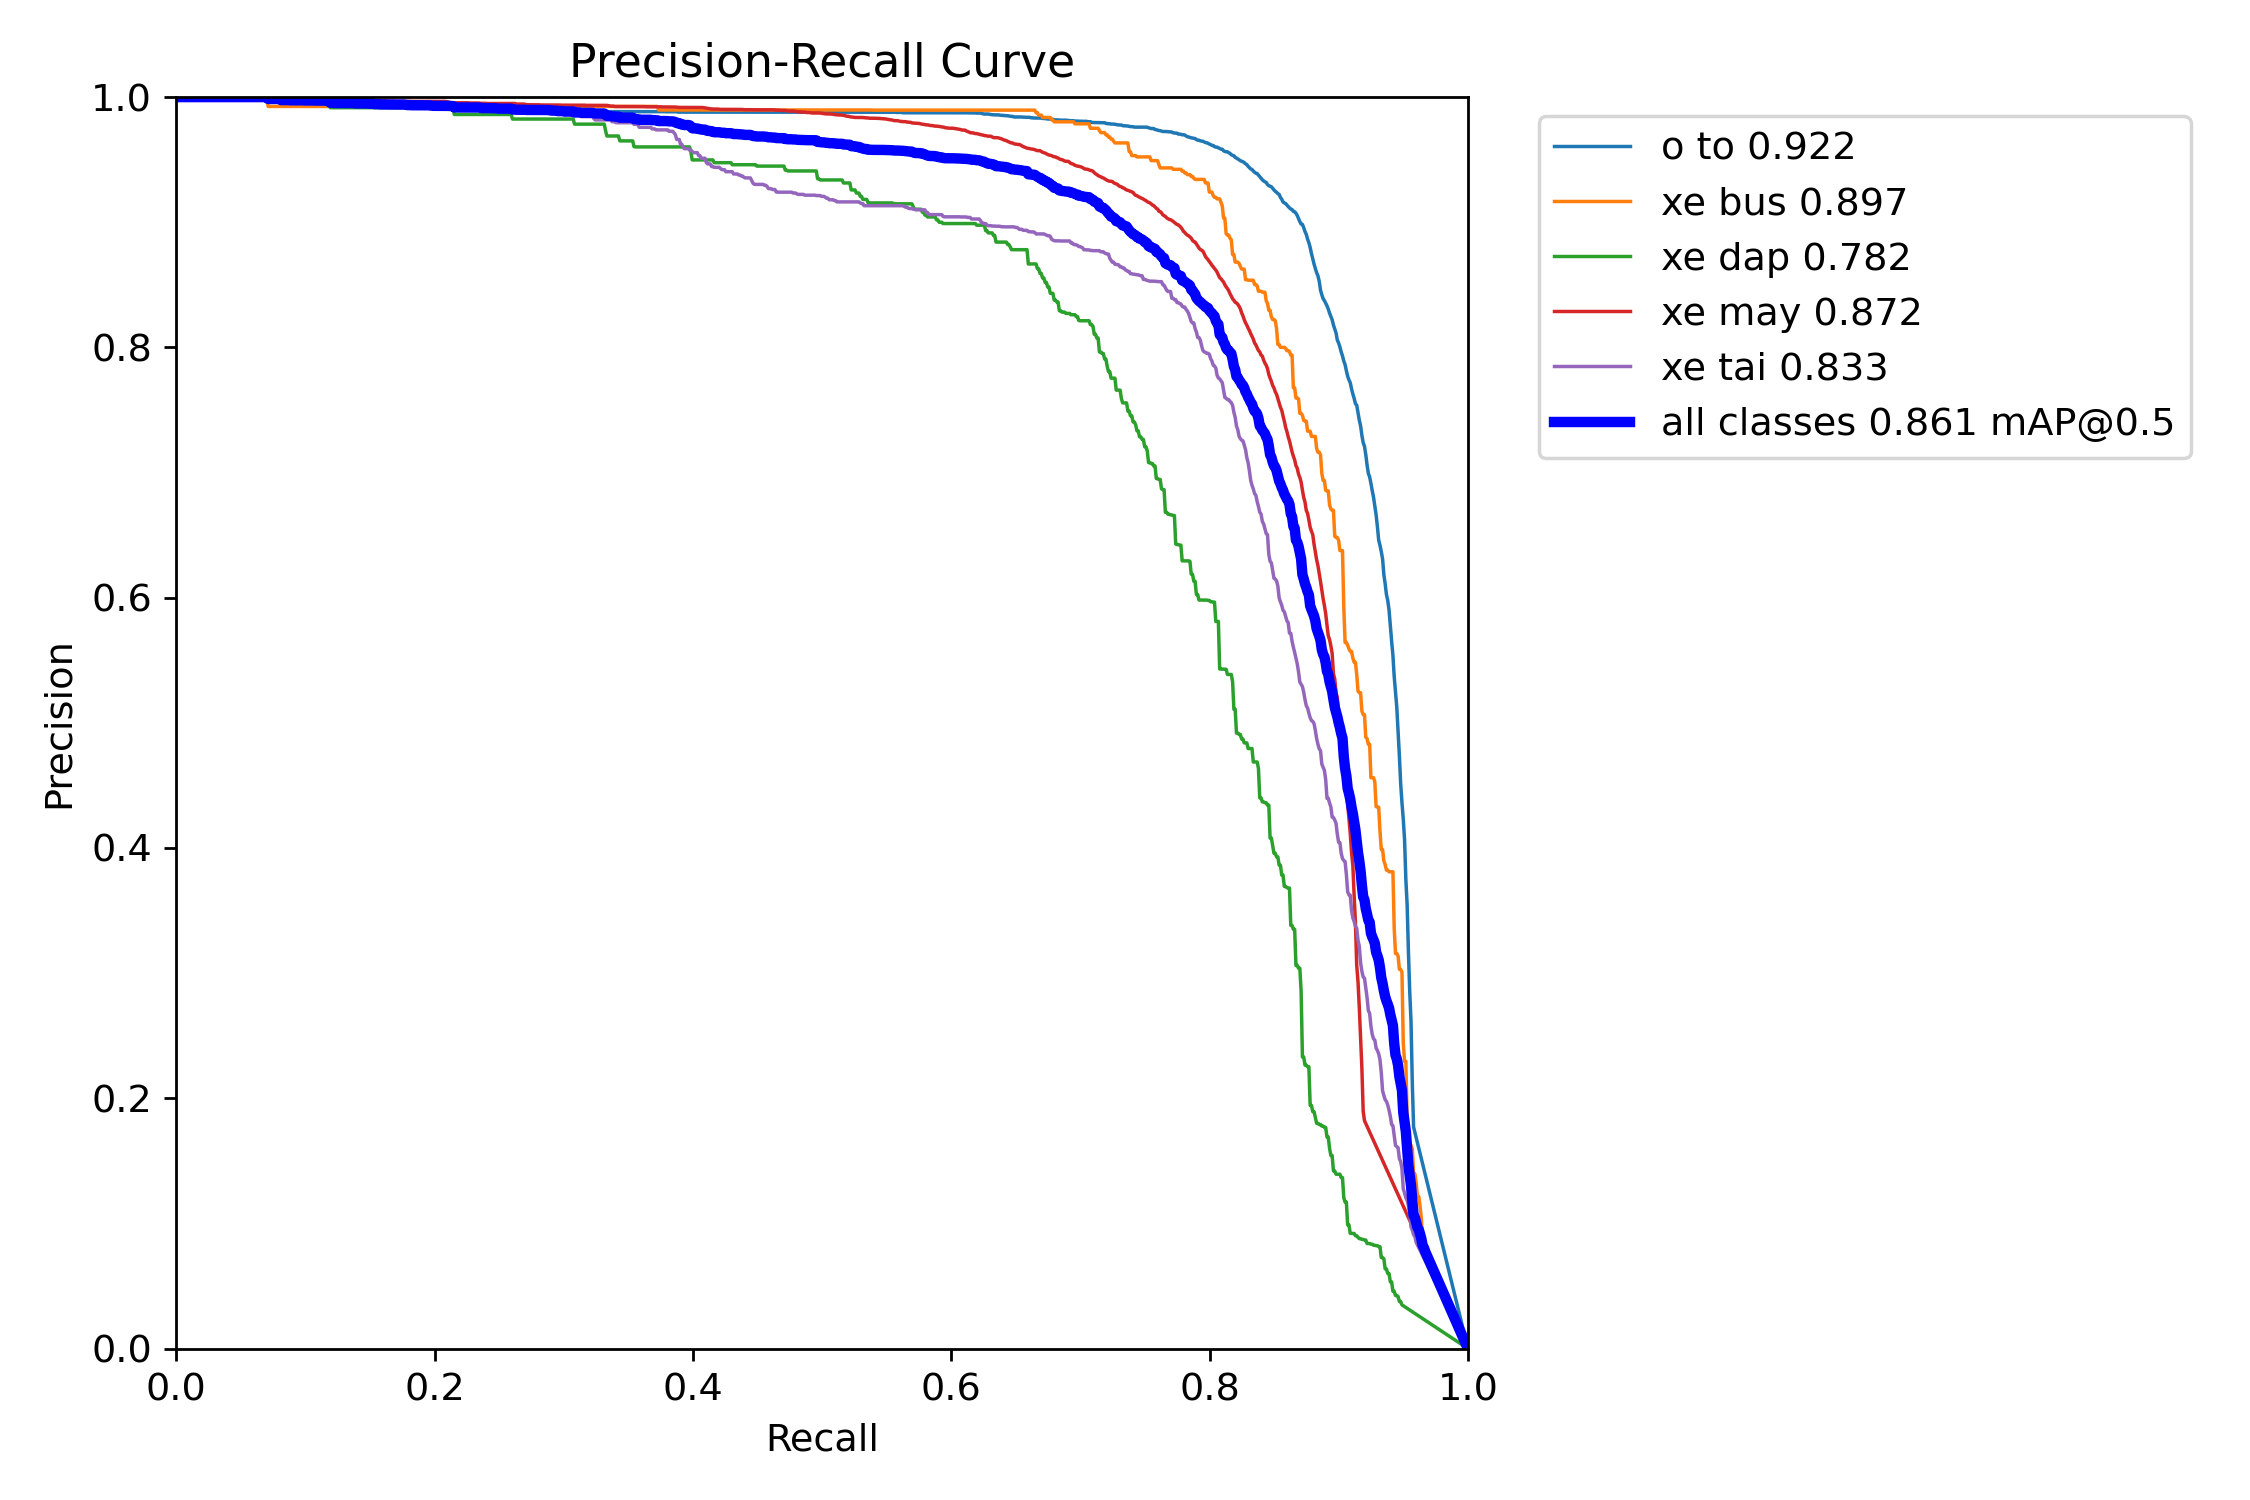
\includegraphics[width=0.8\linewidth]{Figures/BoxPR_curve.png}
    \caption{Đường cong Precision-Recall của Model 1 (Phát hiện phương tiện)}
    \label{fig:vehicle_pr_curve}
\end{figure}

\subsection{Kết quả dự đoán trên tập Validation}
Hình \ref{fig:vehicle_val_pred} minh họa kết quả dự đoán của Model 1 trên tập validation.

\begin{figure}[H]
    \centering
    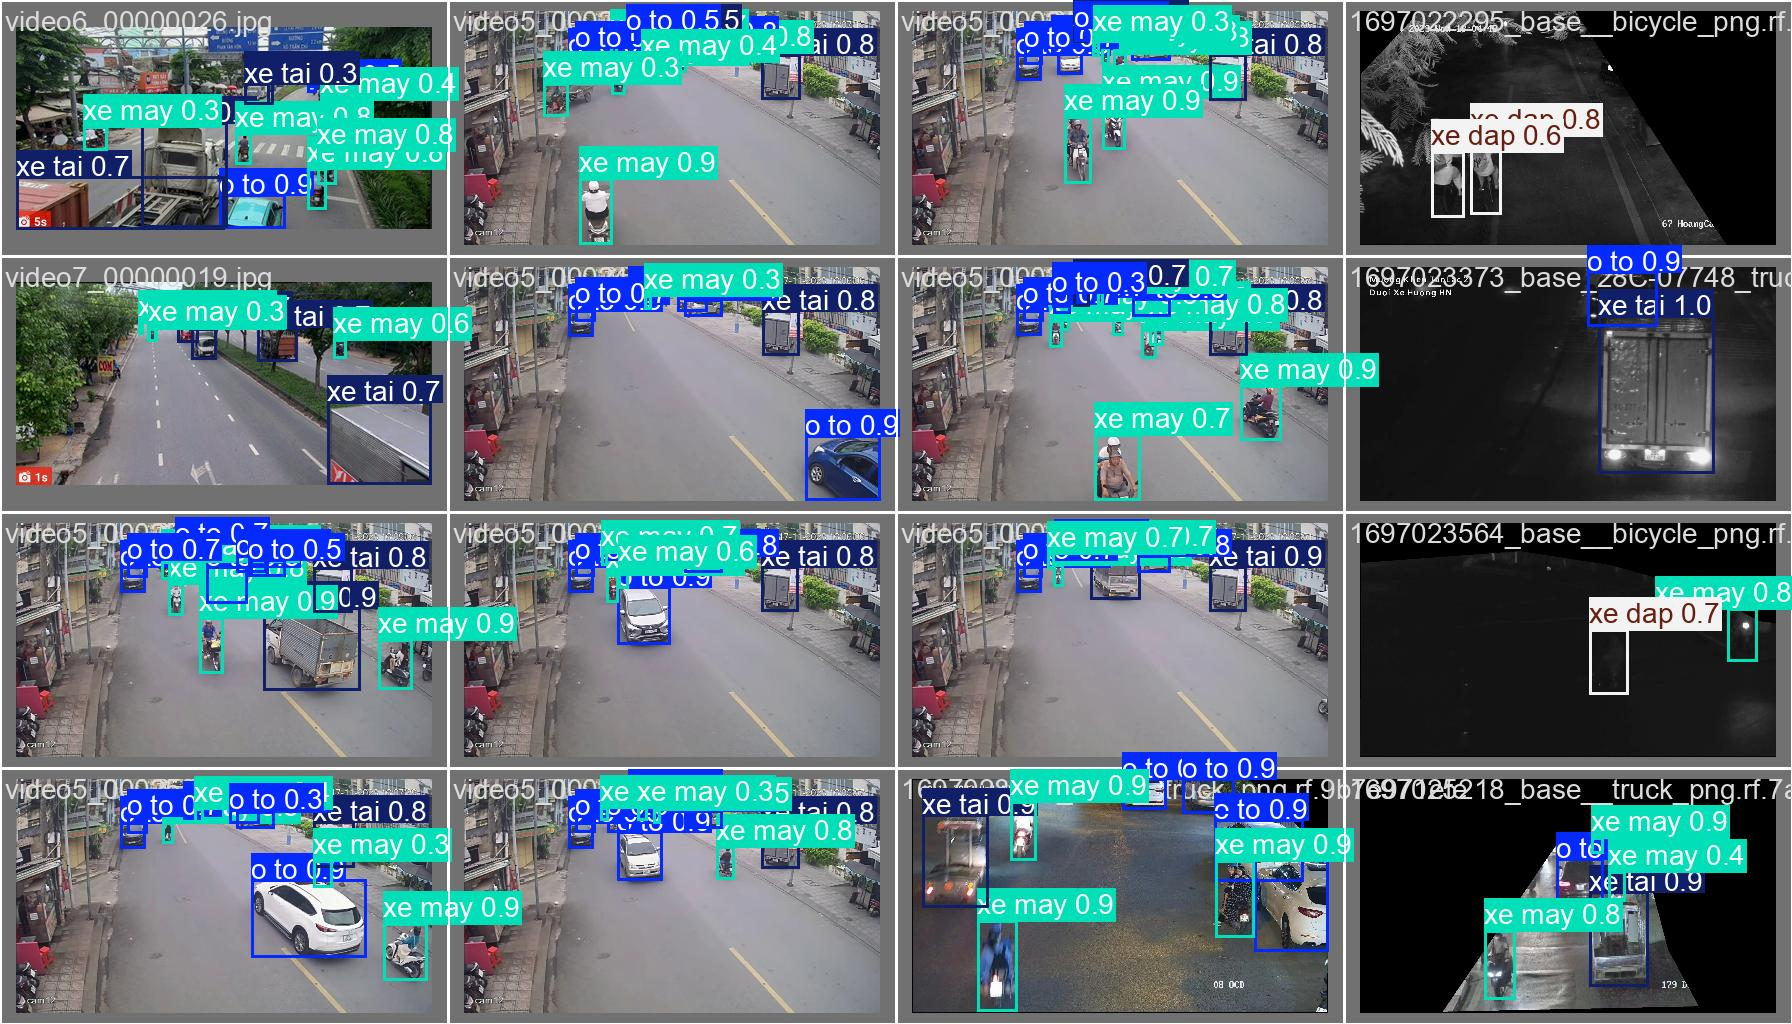
\includegraphics[width=0.95\linewidth]{Figures/val_batch0_pred.jpg}
    \caption{Kết quả dự đoán trên tập Validation - Model 1 (Phát hiện phương tiện)}
    \label{fig:vehicle_val_pred}
\end{figure}



%============================================================
% PHẦN 3: KẾT QUẢ PHÁT HIỆN BIỂN SỐ
%============================================================
\section{Kết quả huấn luyện Plate Detection}

\subsection{Thiết lập huấn luyện}
Mô hình YOLOv11n được huấn luyện trên bộ dữ liệu VNLP với các cấu hình sau:
\begin{itemize}
    \item \textbf{Pretrained model:} YOLOv8 Plate Detector (fine-tuned từ checkpoint)
    \item \textbf{Image size:} 416×416 pixels
    \item \textbf{Batch size:} 16
    \item \textbf{Epochs:} 100
    \item \textbf{Optimizer:} AdamW
    \item \textbf{Patience:} 20 epochs (Early Stopping)
    \item \textbf{Close Mosaic:} 10 epochs cuối
\end{itemize}

\subsection{Quá trình huấn luyện}
Mô hình được huấn luyện trong 100 epochs trên bộ dữ liệu VNLP. Hình \ref{fig:plate_results} thể hiện quá trình hội tụ của các metrics.

\begin{figure}[H]
    \centering
    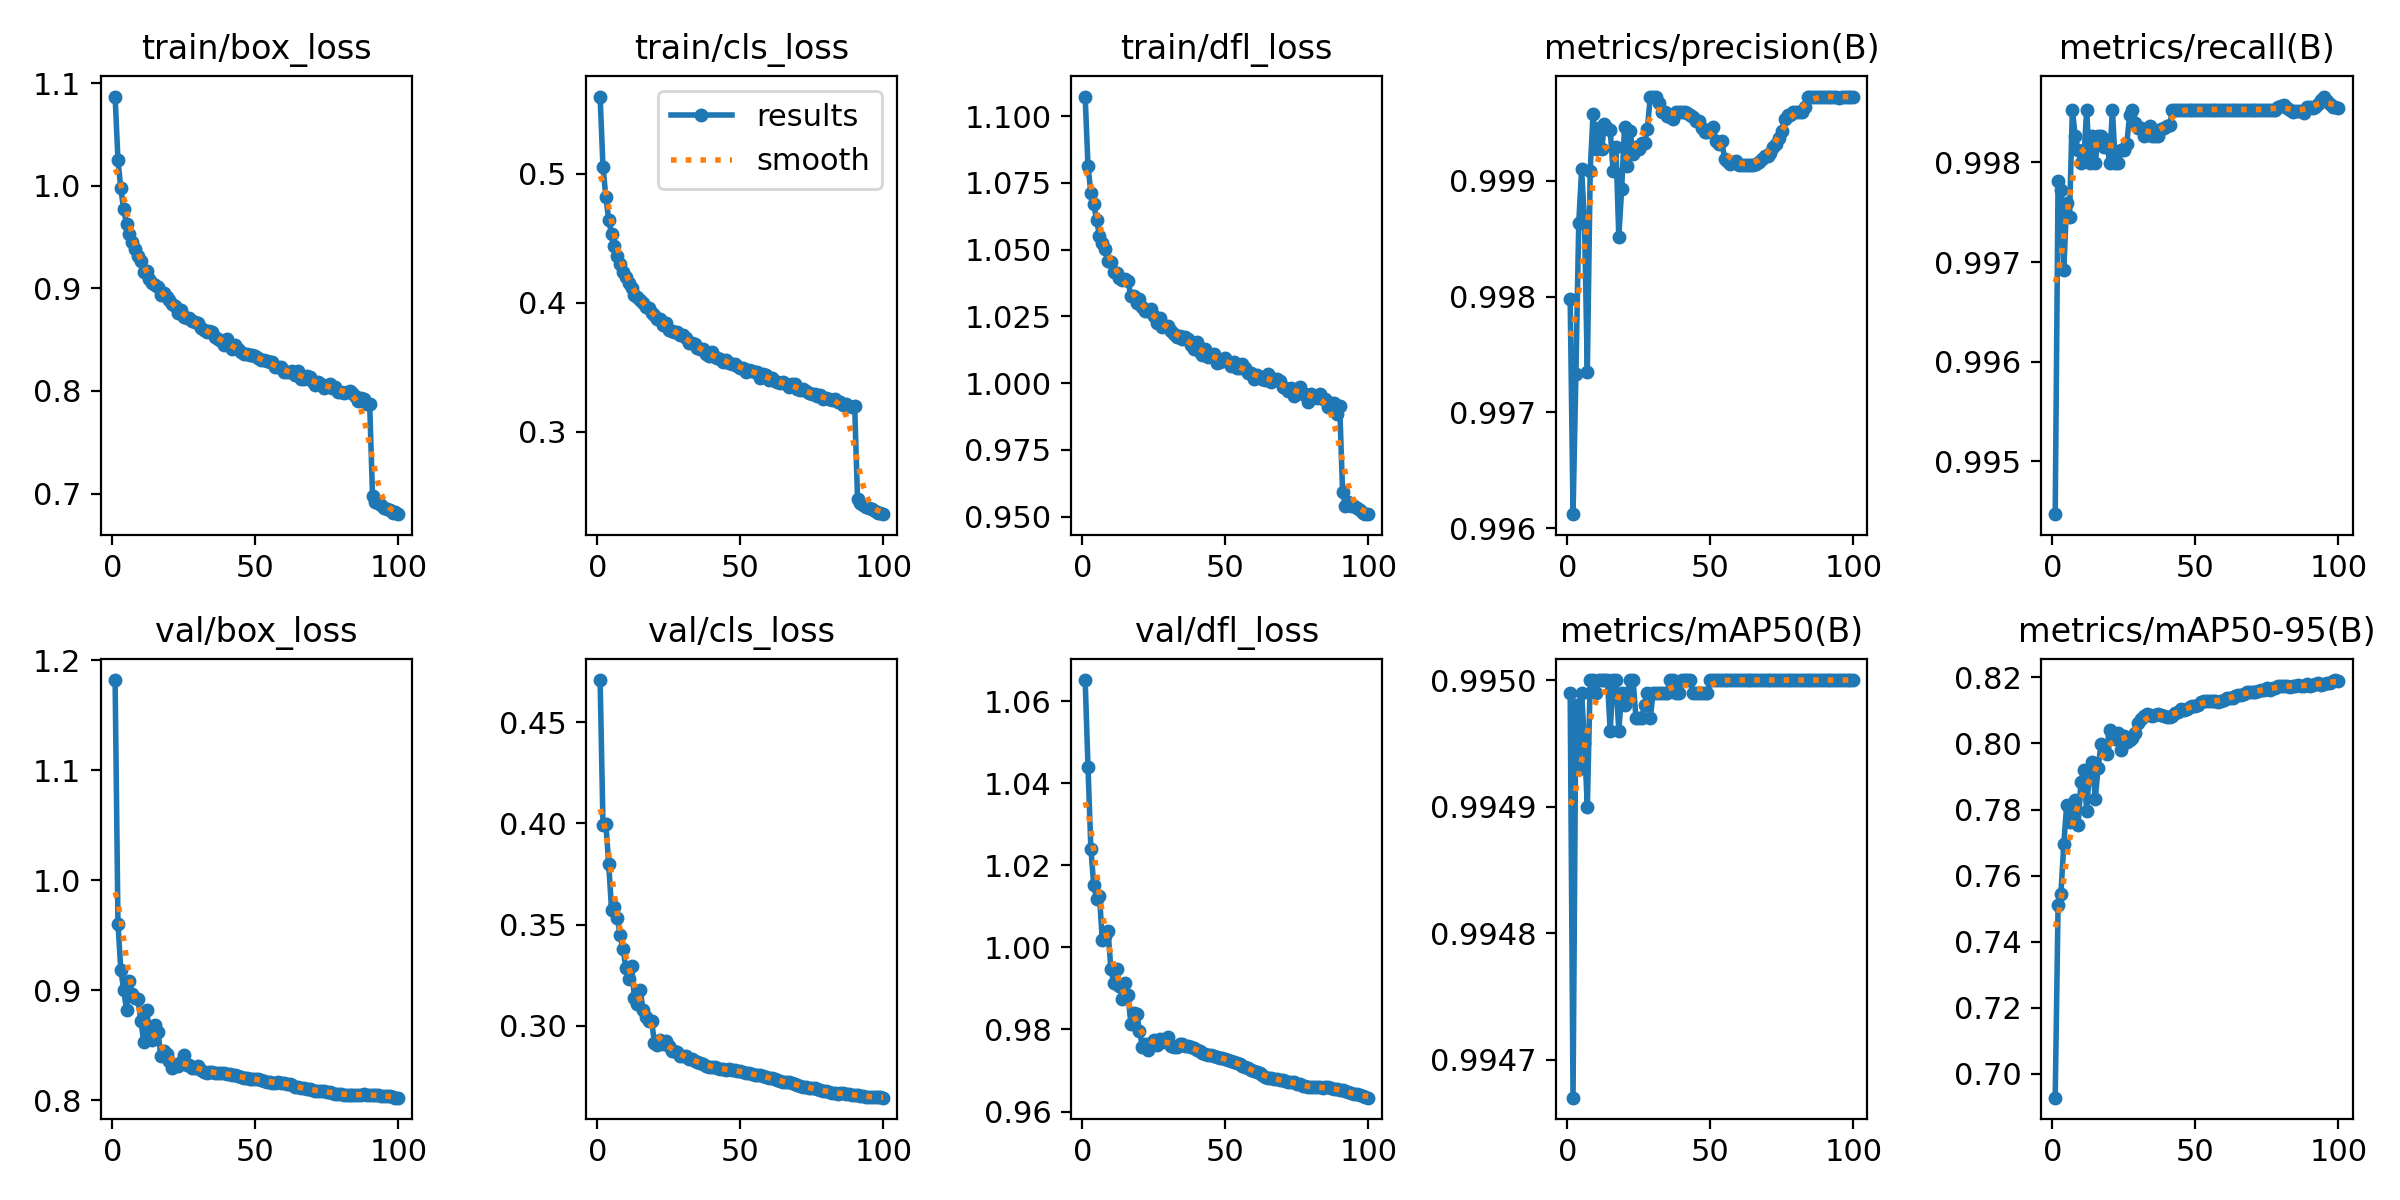
\includegraphics[width=0.95\linewidth]{Figures/plate_results.png}
    \caption{Đường cong Loss và Metrics trong quá trình huấn luyện Plate Detection}
    \label{fig:plate_results}
\end{figure}


\textbf{Nhận xét:}
\begin{itemize}
    \item \textbf{Hội tụ nhanh:} mAP@50 đạt \textbf{99.5\%} ngay từ epoch 1 và duy trì ổn định xuyên suốt quá trình huấn luyện, cho thấy việc sử dụng pretrained weights rất hiệu quả.
    \item \textbf{Loss giảm đều:} Box Loss giảm từ 1.08 xuống 0.68, Classification Loss giảm từ 0.56 xuống 0.24 sau 100 epochs.
    \item \textbf{Không overfitting:} Validation Loss bám sát Training Loss (val\_box\_loss = 0.80, val\_cls\_loss = 0.26).
    \item \textbf{mAP@50-95 tăng dần:} Từ 69.3\% lên \textbf{81.9\%}, cho thấy khả năng localization được cải thiện qua các epochs.
\end{itemize}

\subsection{Kết quả cuối cùng}

\begin{table}[H]
\centering
\caption{Kết quả đánh giá Plate Detection trên tập Validation}
\label{tab:plate_final_results}
\begin{tabular}{|l|c|}
\hline
\textbf{Metric} & \textbf{Giá trị} \\ \hline
Precision & \textbf{99.973\%} \\ \hline
Recall & \textbf{99.855\%} \\ \hline
mAP@50 & \textbf{99.50\%} \\ \hline
mAP@50-95 & \textbf{81.897\%} \\ \hline
\end{tabular}
\end{table}

Mô hình đạt \textbf{Precision = 99.973\%} và \textbf{mAP@50 = 99.50\%}, cho thấy khả năng phát hiện biển số cực kỳ chính xác. Đặc biệt, chỉ số mAP@50-95 đạt \textbf{81.897\%} thể hiện khả năng định vị bounding box rất tốt ở nhiều ngưỡng IoU khác nhau.

\subsection{Ma trận nhầm lẫn Plate Detection}
\begin{figure}[H]
    \centering
    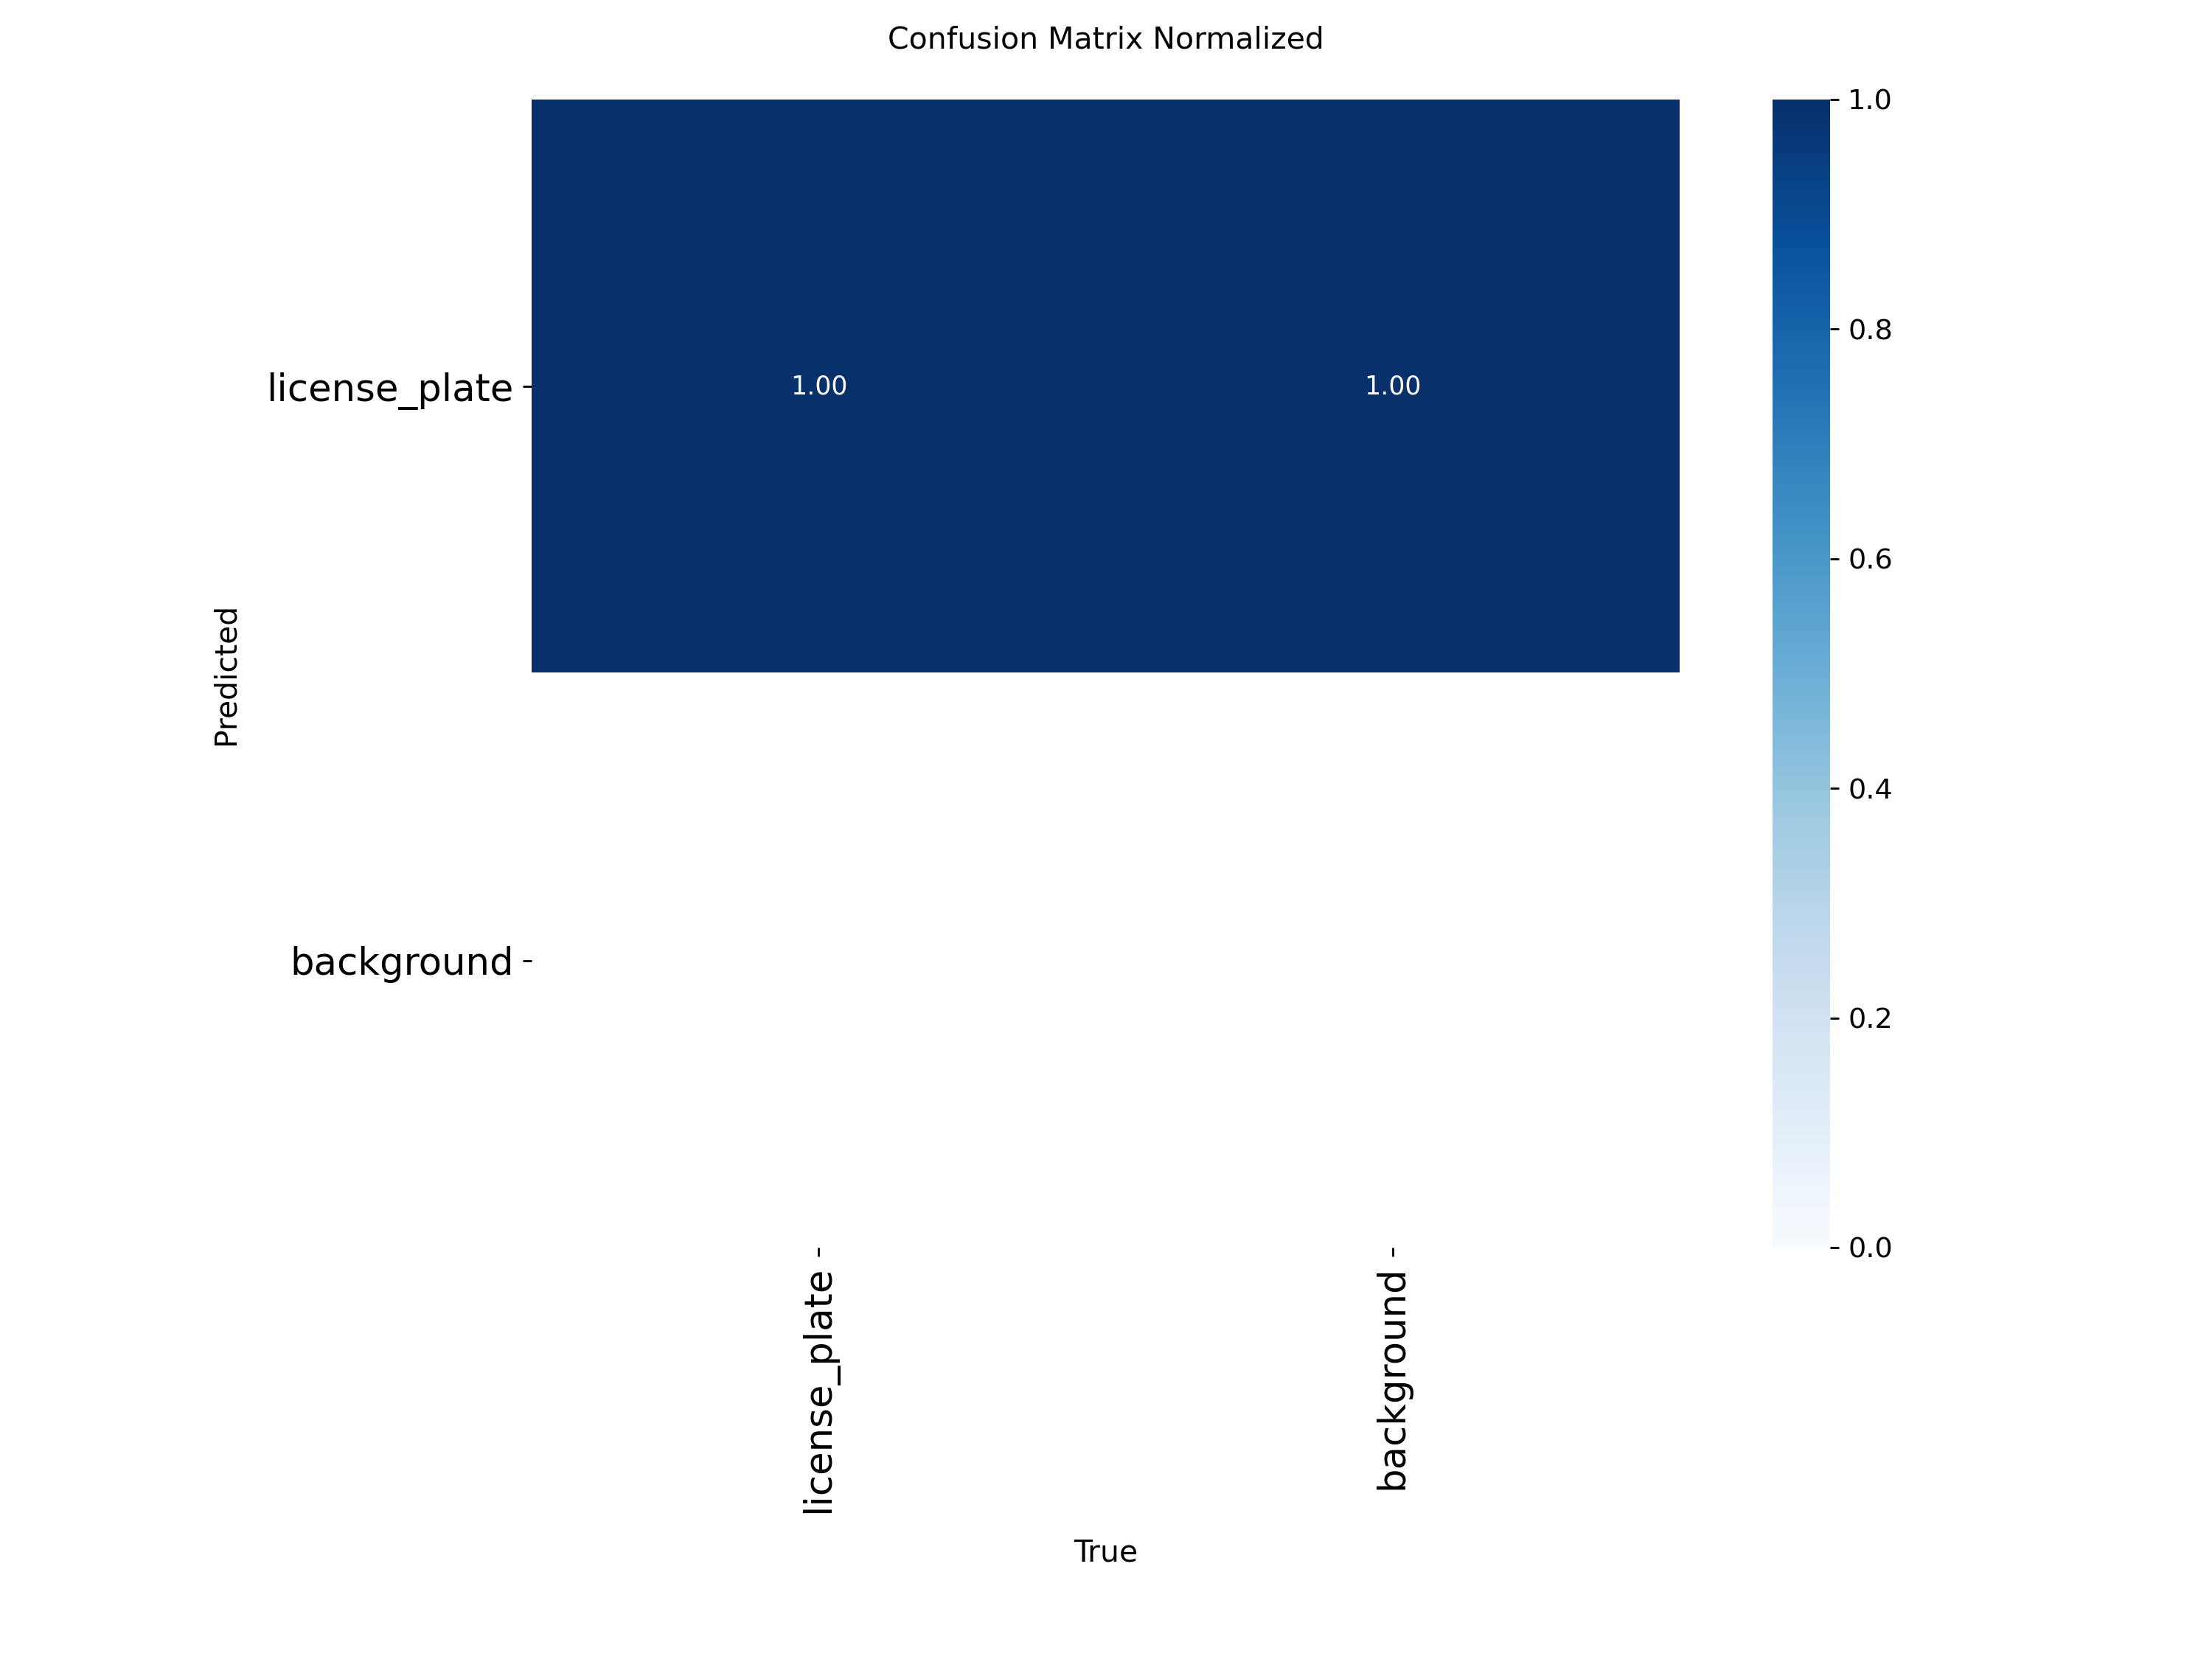
\includegraphics[width=0.6\linewidth]{Figures/plate_confusion_matrix.png}
    \caption{Ma trận nhầm lẫn Plate Detection (Normalized)}
    \label{fig:plate_confusion}
\end{figure}

Ma trận nhầm lẫn chuẩn hóa cho thấy:
\begin{itemize}
    \item \textbf{True Positive Rate:} Gần như \textbf{100\%} biển số được nhận diện đúng.
    \item \textbf{False Negative Rate:} Rất thấp (< 0.2\%), cho thấy mô hình bỏ sót rất ít biển số.
    \item \textbf{False Positive Rate:} Gần như bằng 0, mô hình không nhận nhầm các đối tượng khác là biển số.
\end{itemize}

\subsection{Đường cong Precision-Recall}
Đường cong PR (Hình \ref{fig:plate_pr_curve}) cho thấy mô hình phát hiện biển số đạt hiệu năng gần như hoàn hảo.

\begin{figure}[H]
    \centering
    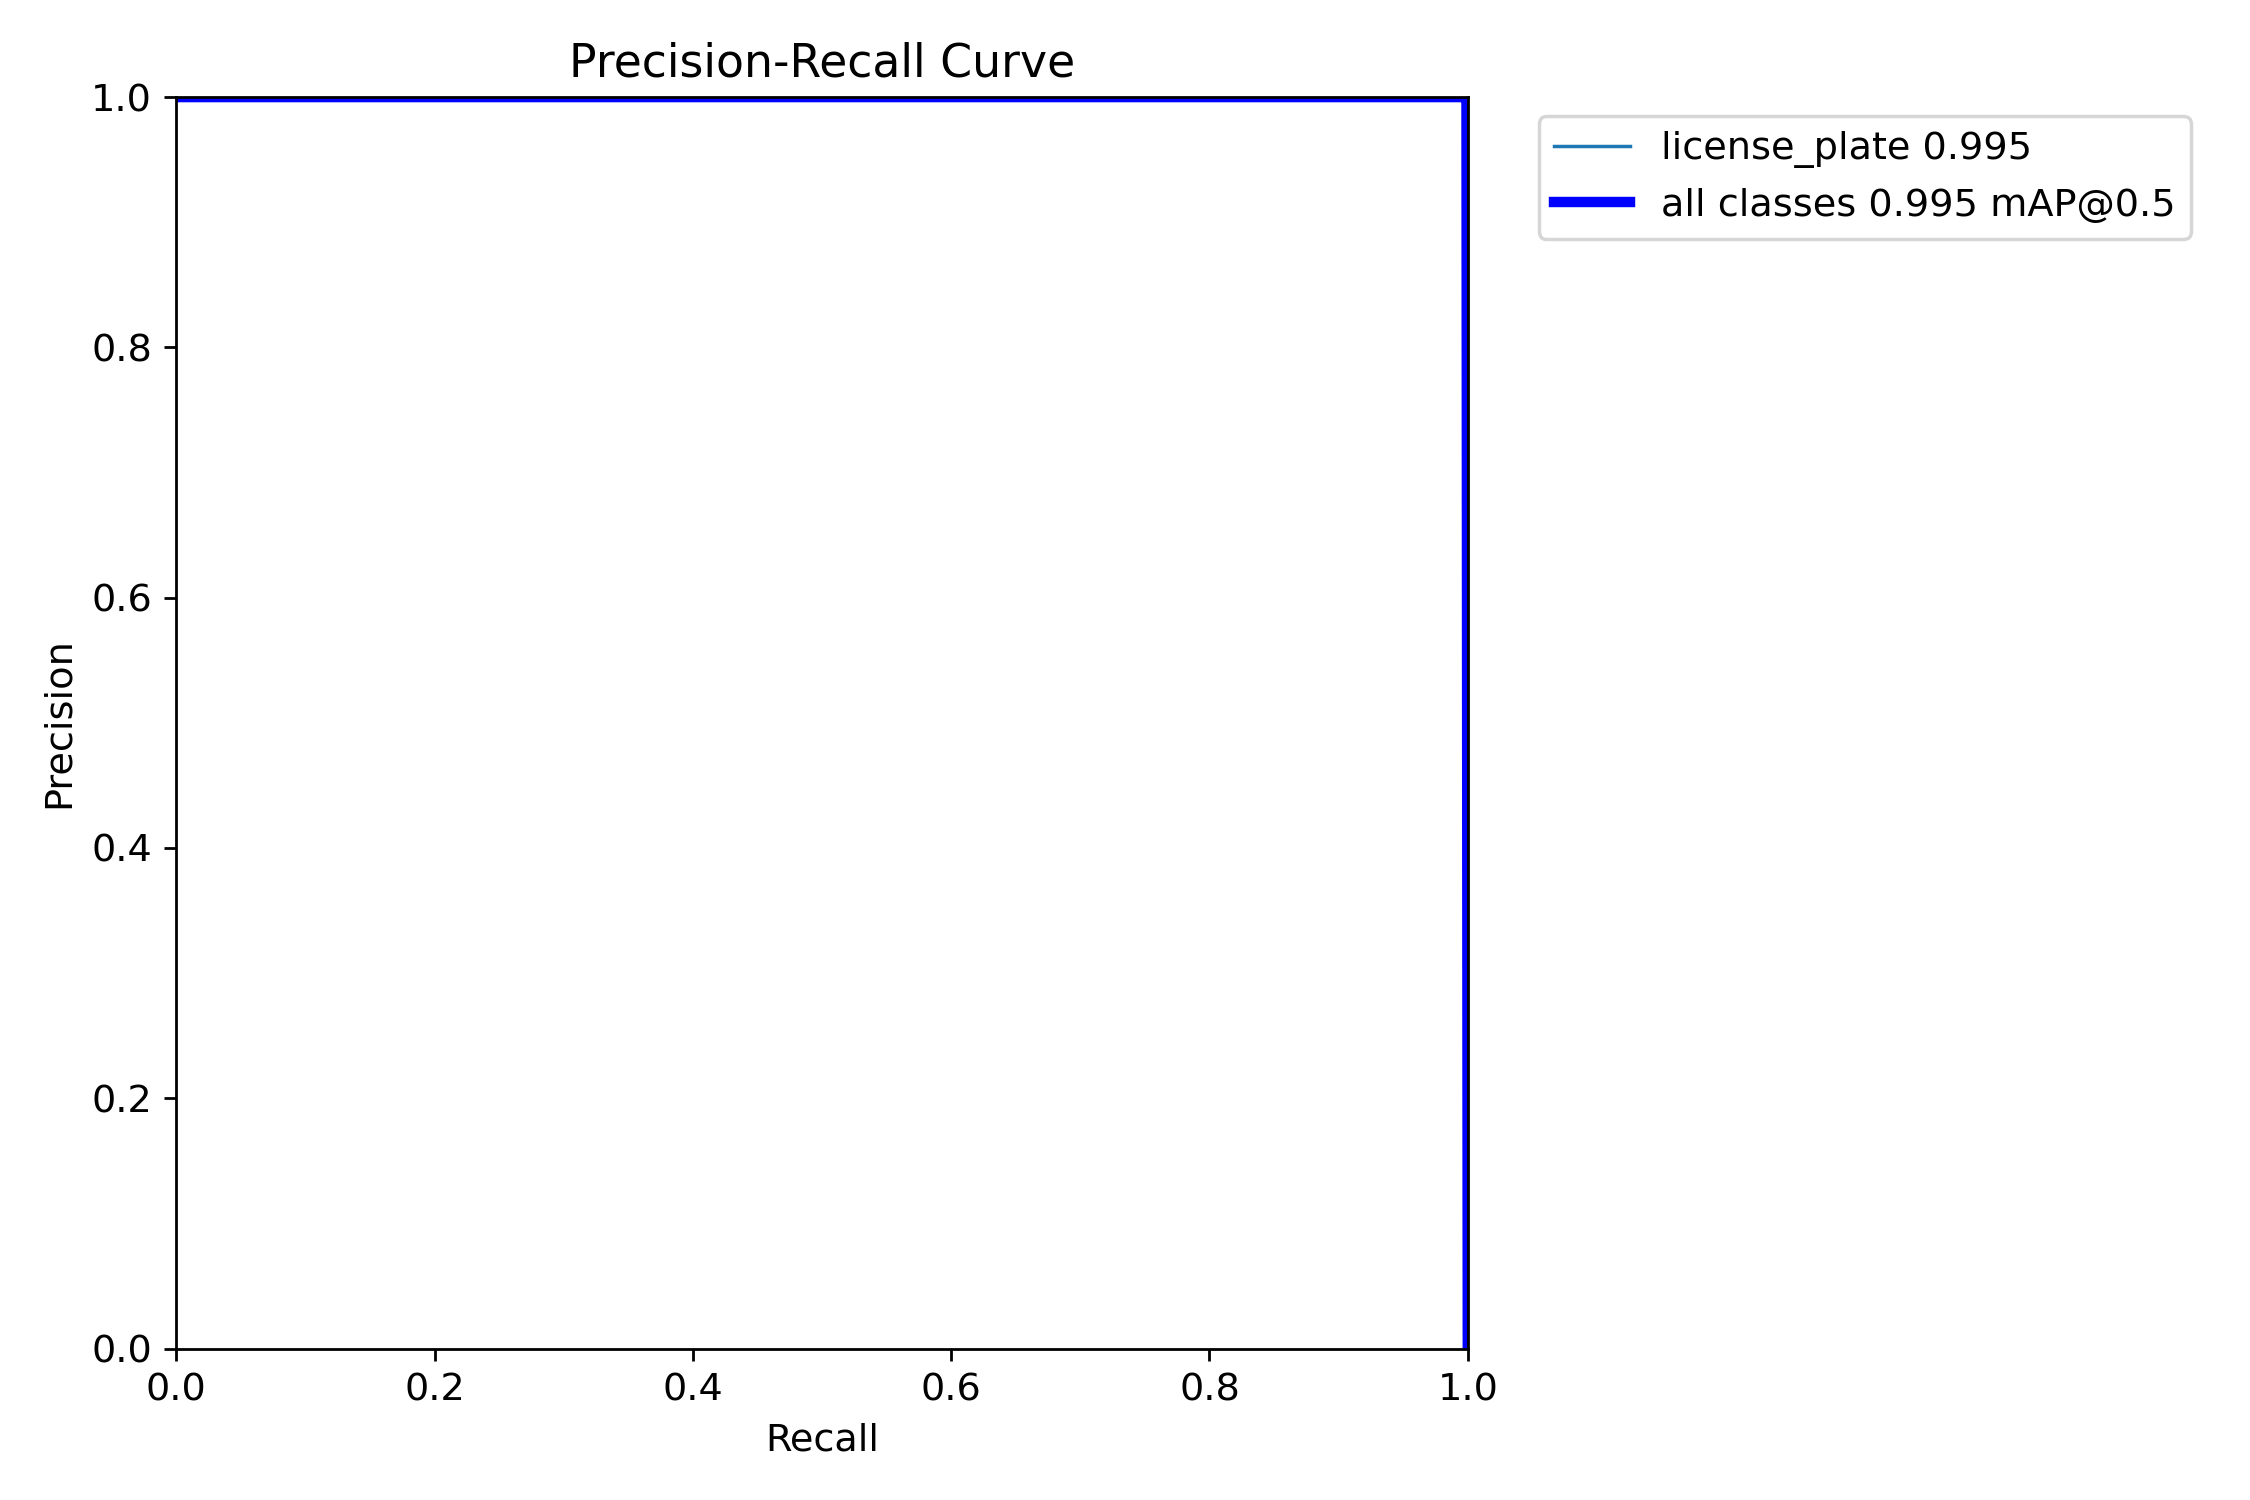
\includegraphics[width=0.8\linewidth]{Figures/plate_PR_curve.png}
    \caption{Đường cong Precision-Recall của Model 2 (Phát hiện biển số)}
    \label{fig:plate_pr_curve}
\end{figure}

\textbf{Nhận xét:}
\begin{itemize}
    \item Đường cong gần như nằm ở góc trên-phải, thể hiện cả Precision và Recall đều rất cao.
    \item \textbf{AP (Average Precision) = 99.5\%}, diện tích dưới đường cong gần bằng 1.0.
    \item Mô hình duy trì Precision > 99\% ngay cả khi Recall tiến tới 100\%.
\end{itemize}

\subsection{Kết quả dự đoán trên tập Validation}
Hình \ref{fig:plate_val_pred} minh họa kết quả dự đoán của Model 2 trên tập validation.

\begin{figure}[H]
    \centering
    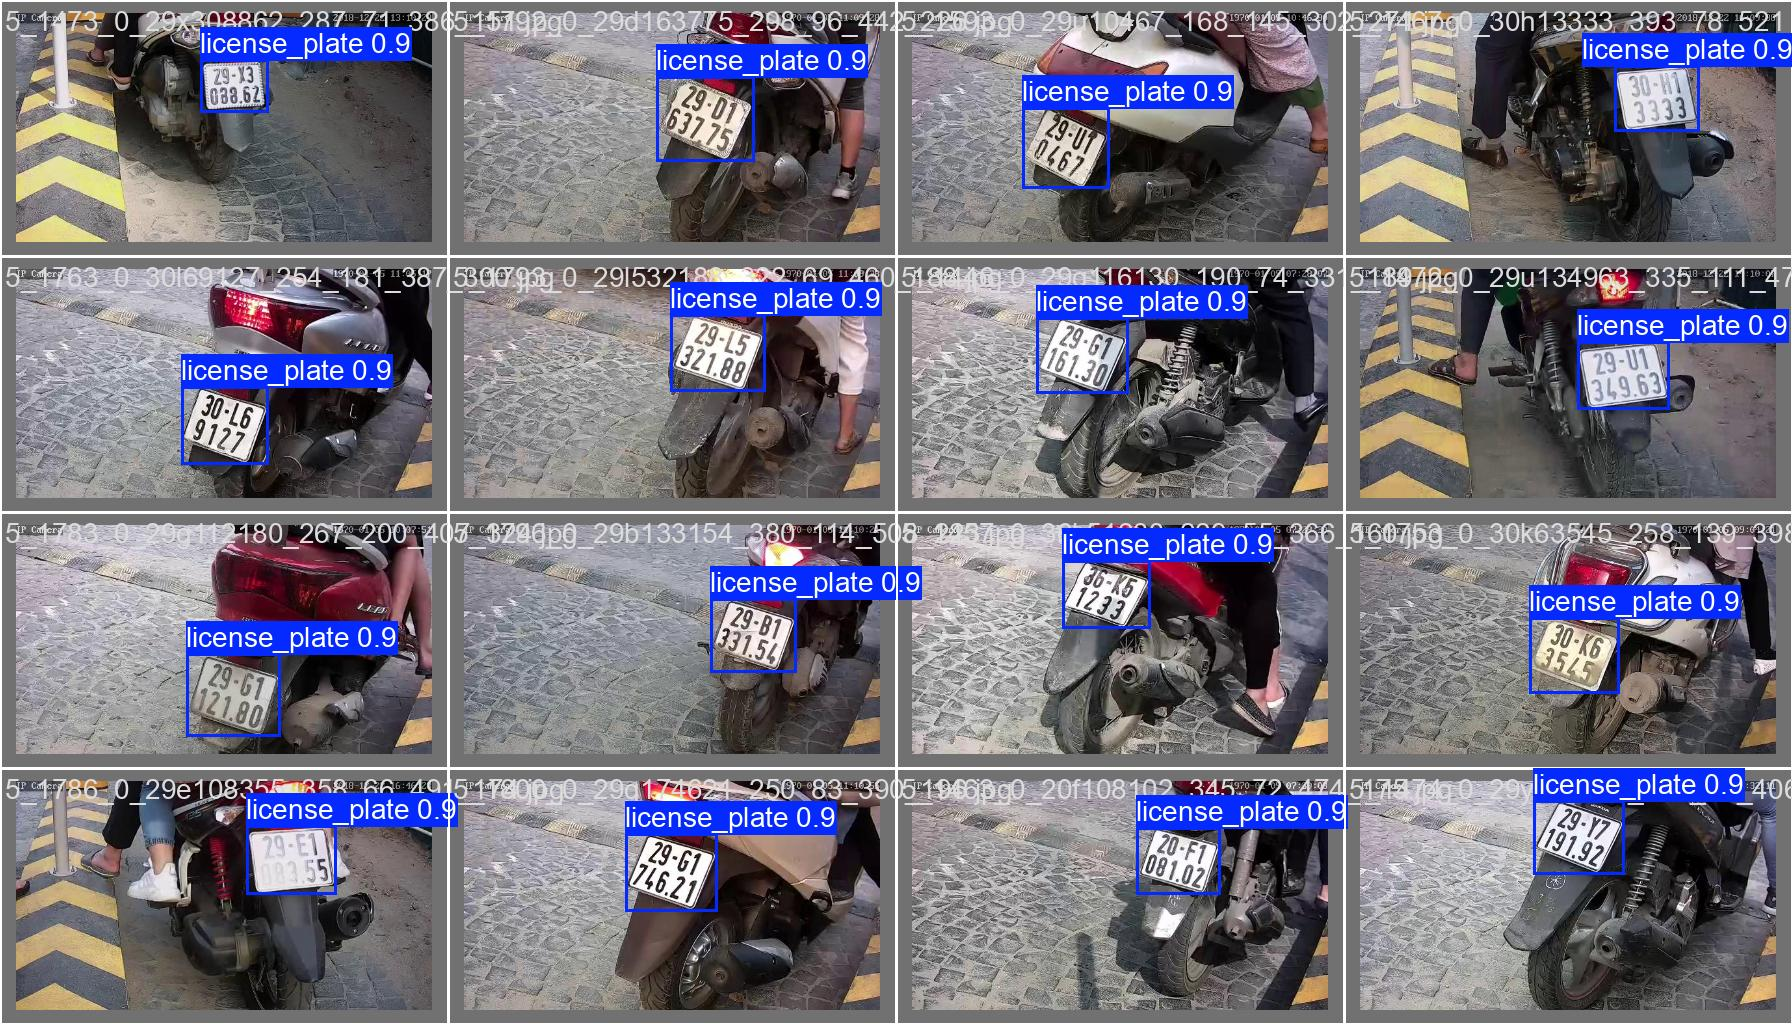
\includegraphics[width=0.95\linewidth]{Figures/plate_val_pred.jpg}
    \caption{Kết quả dự đoán trên tập Validation - Model 2 (Phát hiện biển số)}
    \label{fig:plate_val_pred}
\end{figure}

\textbf{Nhận xét:}
\begin{itemize}
    \item Mô hình phát hiện chính xác biển số xe trong nhiều điều kiện: góc chụp khác nhau, ánh sáng thay đổi, khoảng cách xa/gần.
    \item Bounding box bám sát biển số với độ tin cậy (confidence) > 0.9 cho hầu hết các trường hợp.
    \item Khả năng phát hiện biển số bị một phần che khuất vẫn tốt nhờ dữ liệu huấn luyện đa dạng.
\end{itemize}

%============================================================
% PHẦN 4: KẾT QUẢ MÔ HÌNH TÍCH HỢP (6 LỚP)
%============================================================
\section{Kết quả huấn luyện Mô hình tích hợp (6 lớp)}

\subsection{Kết quả định lượng}
Mô hình tích hợp (6 lớp: 5 loại xe + biển số) được huấn luyện trên dataset được gán nhãn bán giám sát trong 100 epochs. Kết quả tổng hợp trên tất cả các lớp:

\begin{table}[H]
\centering
\caption{Kết quả huấn luyện Mô hình tích hợp 6 lớp}
\label{tab:multiclass_results}
\begin{tabular}{|l|c|}
\hline
\textbf{Metric (All Classes)} & \textbf{Giá trị} \\ \hline
Precision & 84.7\% \\ \hline
Recall & 71.6\% \\ \hline
mAP@50 & 78.5\% \\ \hline
mAP@50-95 & 62.3\% \\ \hline
\end{tabular}
\end{table}

So với mô hình chuyên biệt (Phương pháp 1) đạt mAP@50 99.5\%, mô hình tích hợp có độ chính xác thấp hơn do phải giải quyết bài toán khó hơn (multiclass imbalance). Tuy nhiên, lợi thế là tốc độ inference nhanh hơn do gom 2 bước detection thành 1.

\subsection{Kết quả chi tiết theo từng lớp của mô hình tích hợp}

\begin{table}[H]
\centering
\caption{Kết quả mAP@50 theo từng lớp của mô hình tích hợp 6 lớp}
\label{tab:multiclass_per_class}
\begin{tabular}{|l|c|c|c|}
\hline
\textbf{Lớp} & \textbf{mAP@50} & \textbf{Precision} & \textbf{Recall} \\ \hline
Ô tô (o to) & 0.89 & 0.88 & 0.82 \\ \hline
Xe buýt (xe bus) & 0.86 & 0.85 & 0.78 \\ \hline
Xe đạp (xe dap) & 0.72 & 0.75 & 0.65 \\ \hline
Xe máy (xe may) & 0.84 & 0.83 & 0.76 \\ \hline
Xe tải (xe tai) & 0.81 & 0.82 & 0.73 \\ \hline
Biển số (plate) & 0.59 & 0.72 & 0.56 \\ \hline
\end{tabular}
\end{table}

\textbf{Nhận xét:} Lớp ``plate'' (biển số) có kết quả thấp nhất (mAP@50 = 0.59) do:
\begin{itemize}
    \item \textbf{Class imbalance:} Số lượng biển số ít hơn nhiều so với các lớp phương tiện
    \item \textbf{Kích thước nhỏ:} Biển số thường chiếm diện tích rất nhỏ trong ảnh
    \item \textbf{Tỷ lệ annotation:} Dữ liệu gán nhãn tự động (semi-supervised) có thể bỏ sót một số biển nhỏ/mờ
\end{itemize}

\subsection{Đánh giá trực quan}

\begin{figure}[H]
    \centering
    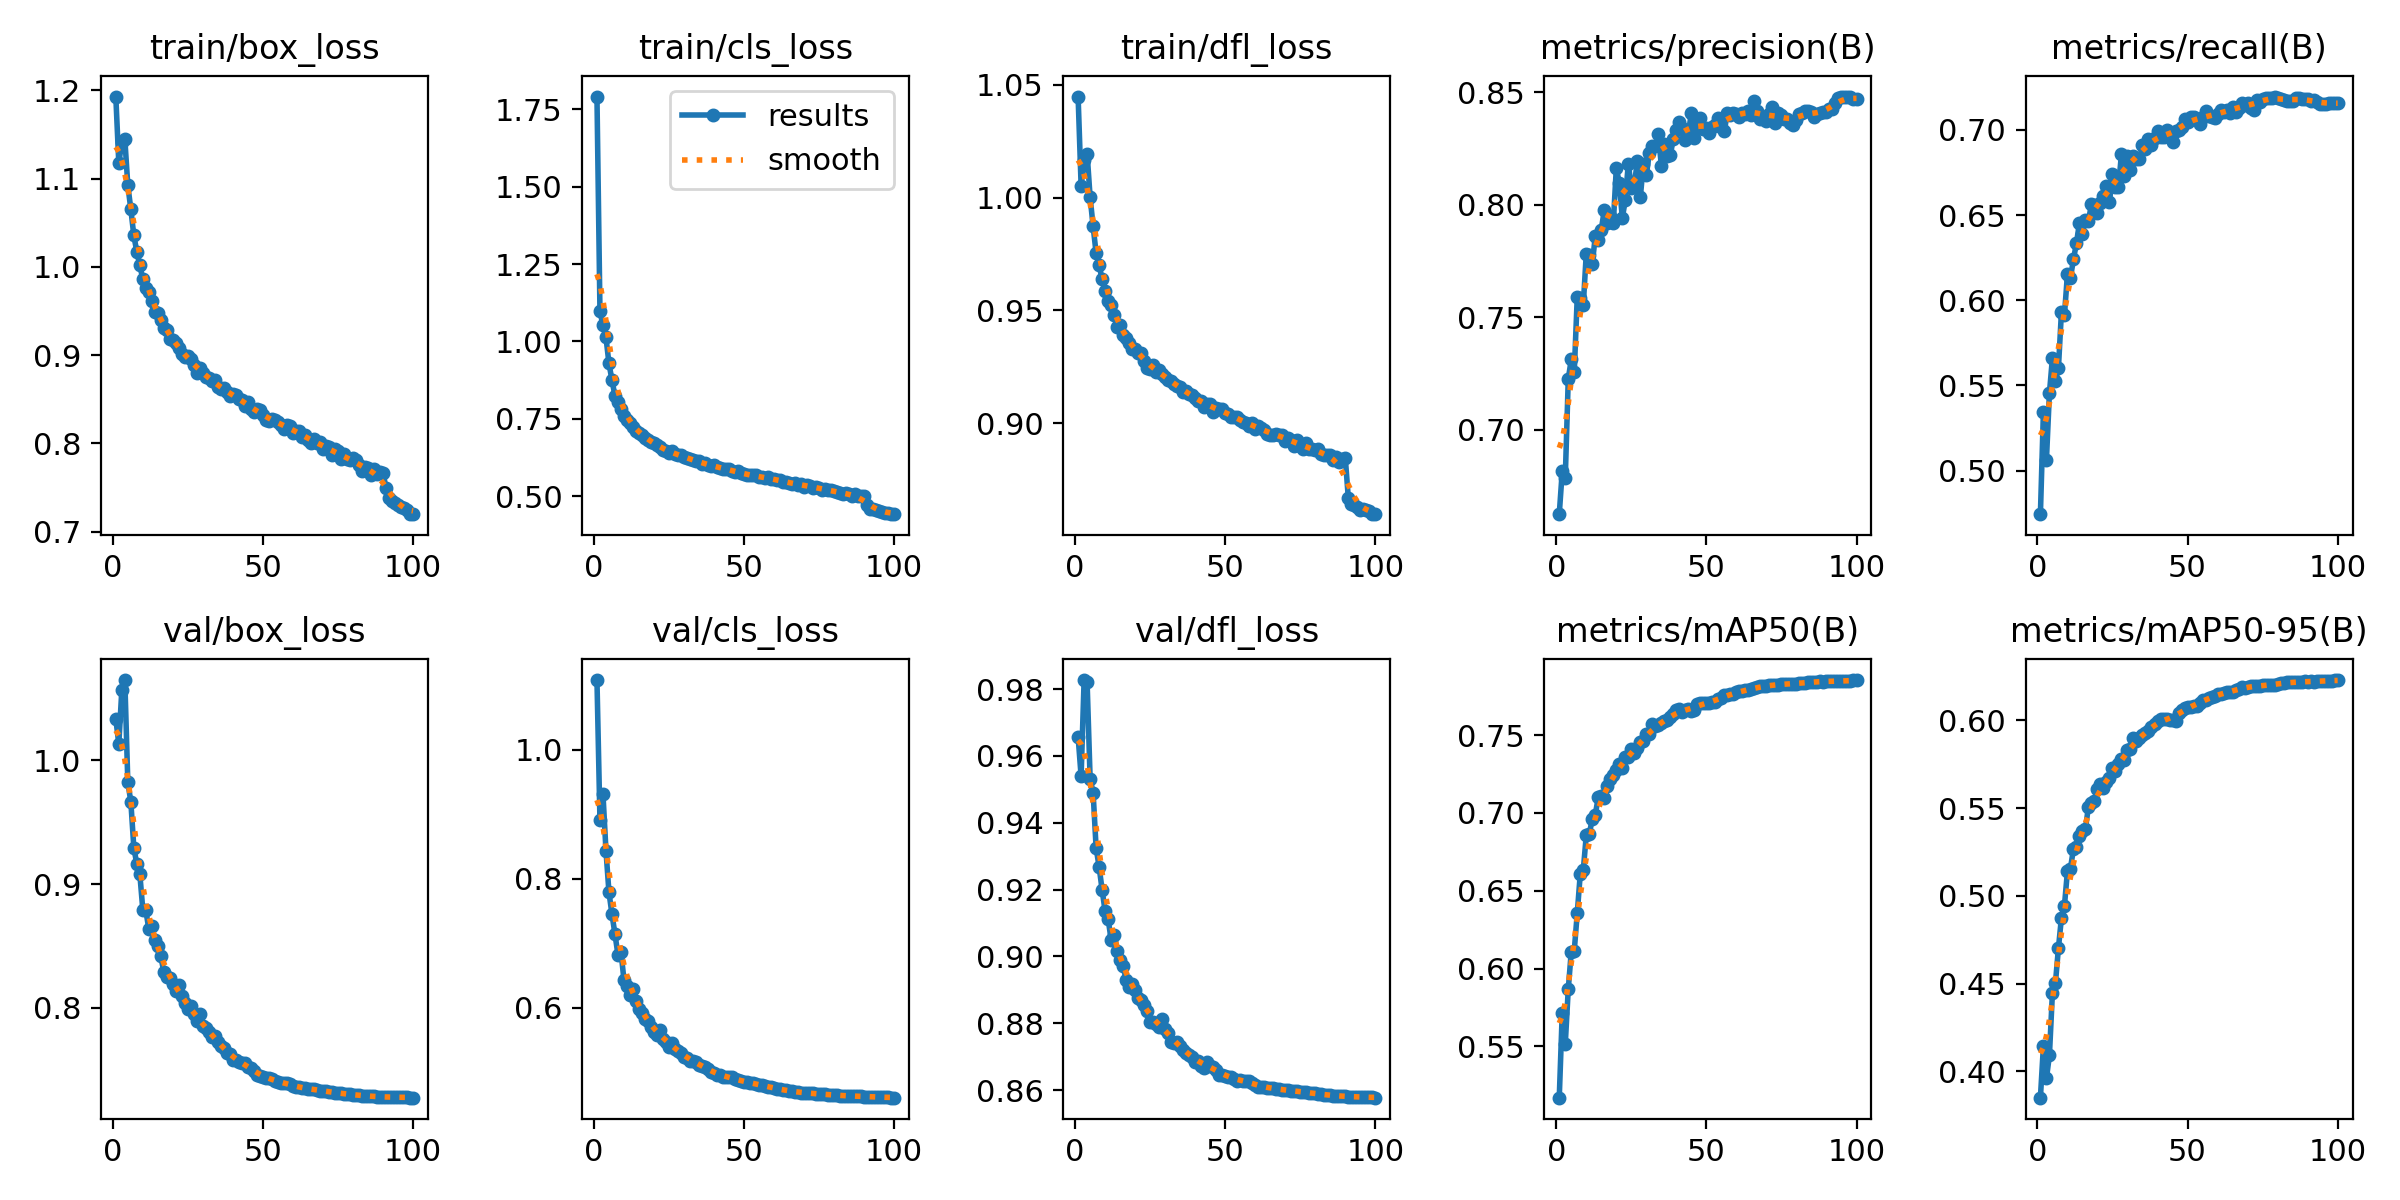
\includegraphics[width=0.95\linewidth]{Figures/multiclass_results.png}
    \caption{Đường cong Loss và Metrics của mô hình tích hợp 6 lớp}
    \label{fig:multiclass_results}
\end{figure}

\subsection{Ma trận nhầm lẫn mô hình tích hợp}

\begin{figure}[H]
    \centering
    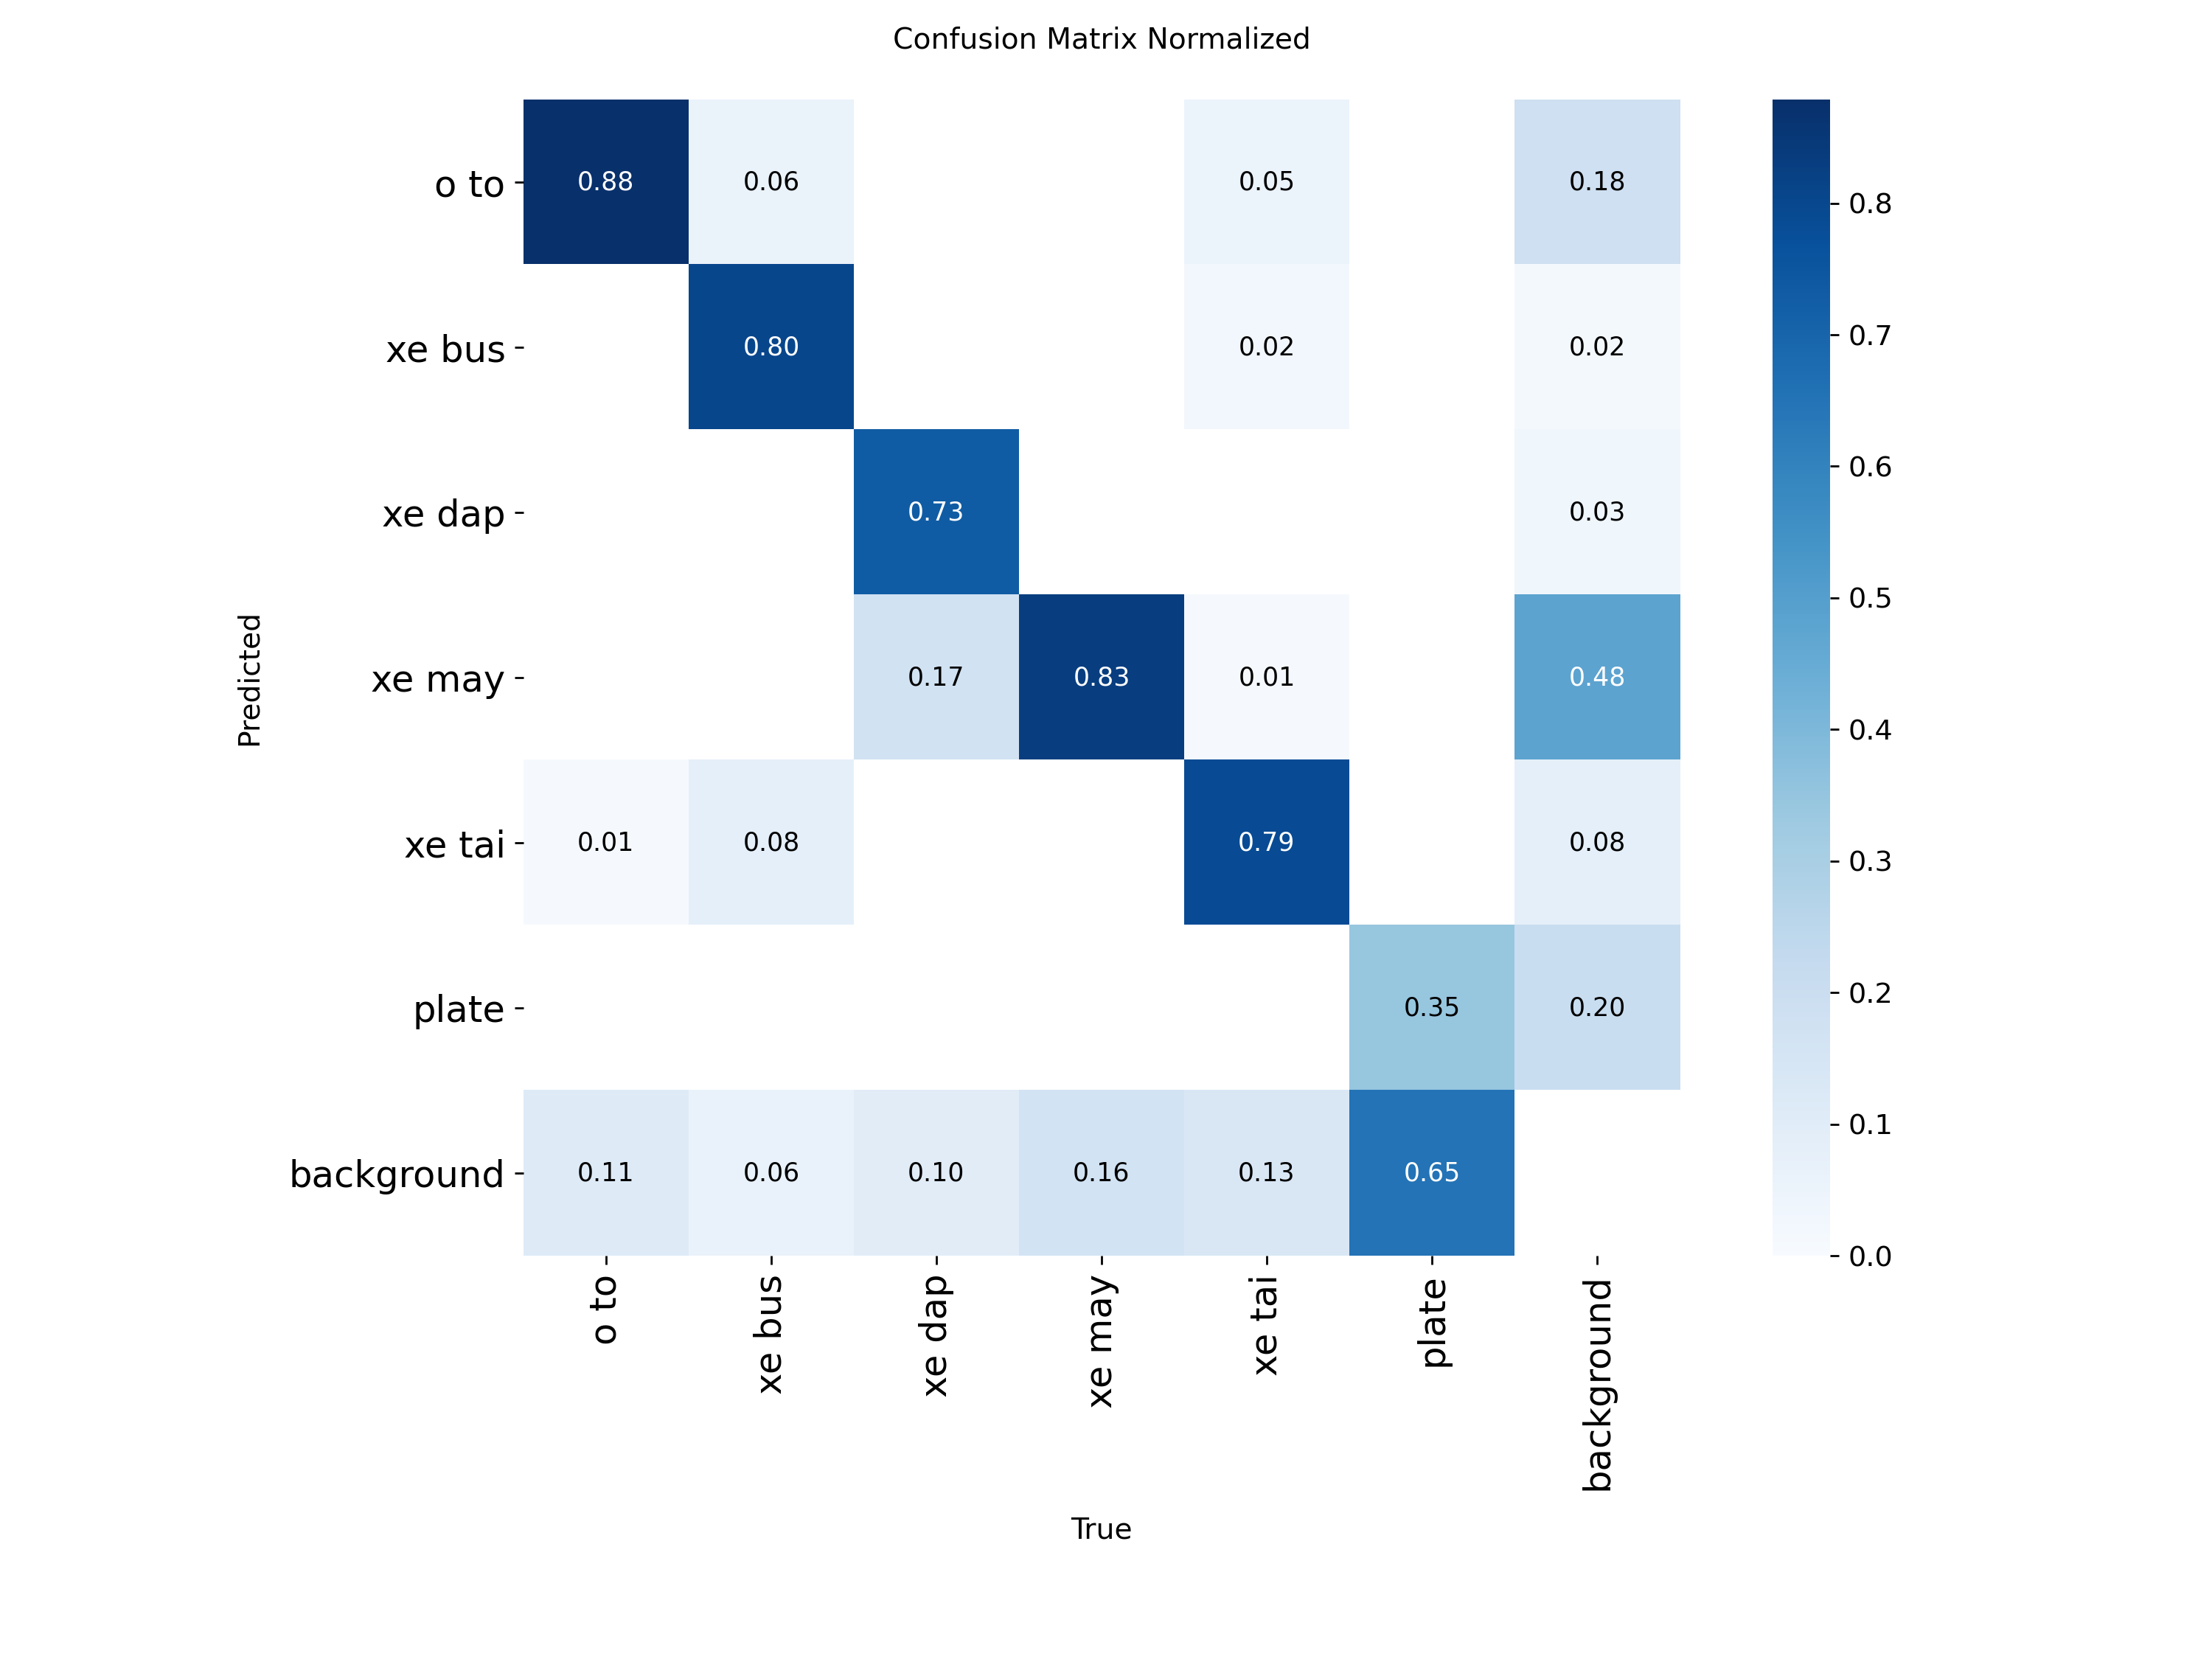
\includegraphics[width=0.75\linewidth]{Figures/multiclass_confusion.png}
    \caption{Ma trận nhầm lẫn của mô hình tích hợp 6 lớp (Normalized)}
    \label{fig:multiclass_confusion}
\end{figure}

Ma trận nhầm lẫn (Hình \ref{fig:multiclass_confusion}) cho thấy các lớp phương tiện vẫn giữ được độ chính xác tốt, tuy nhiên lớp ``plate'' có tỷ lệ bỏ sót (False Negative) cao hơn do kích thước nhỏ.

\subsection{Đường cong Precision-Recall mô hình tích hợp}

\begin{figure}[H]
    \centering
    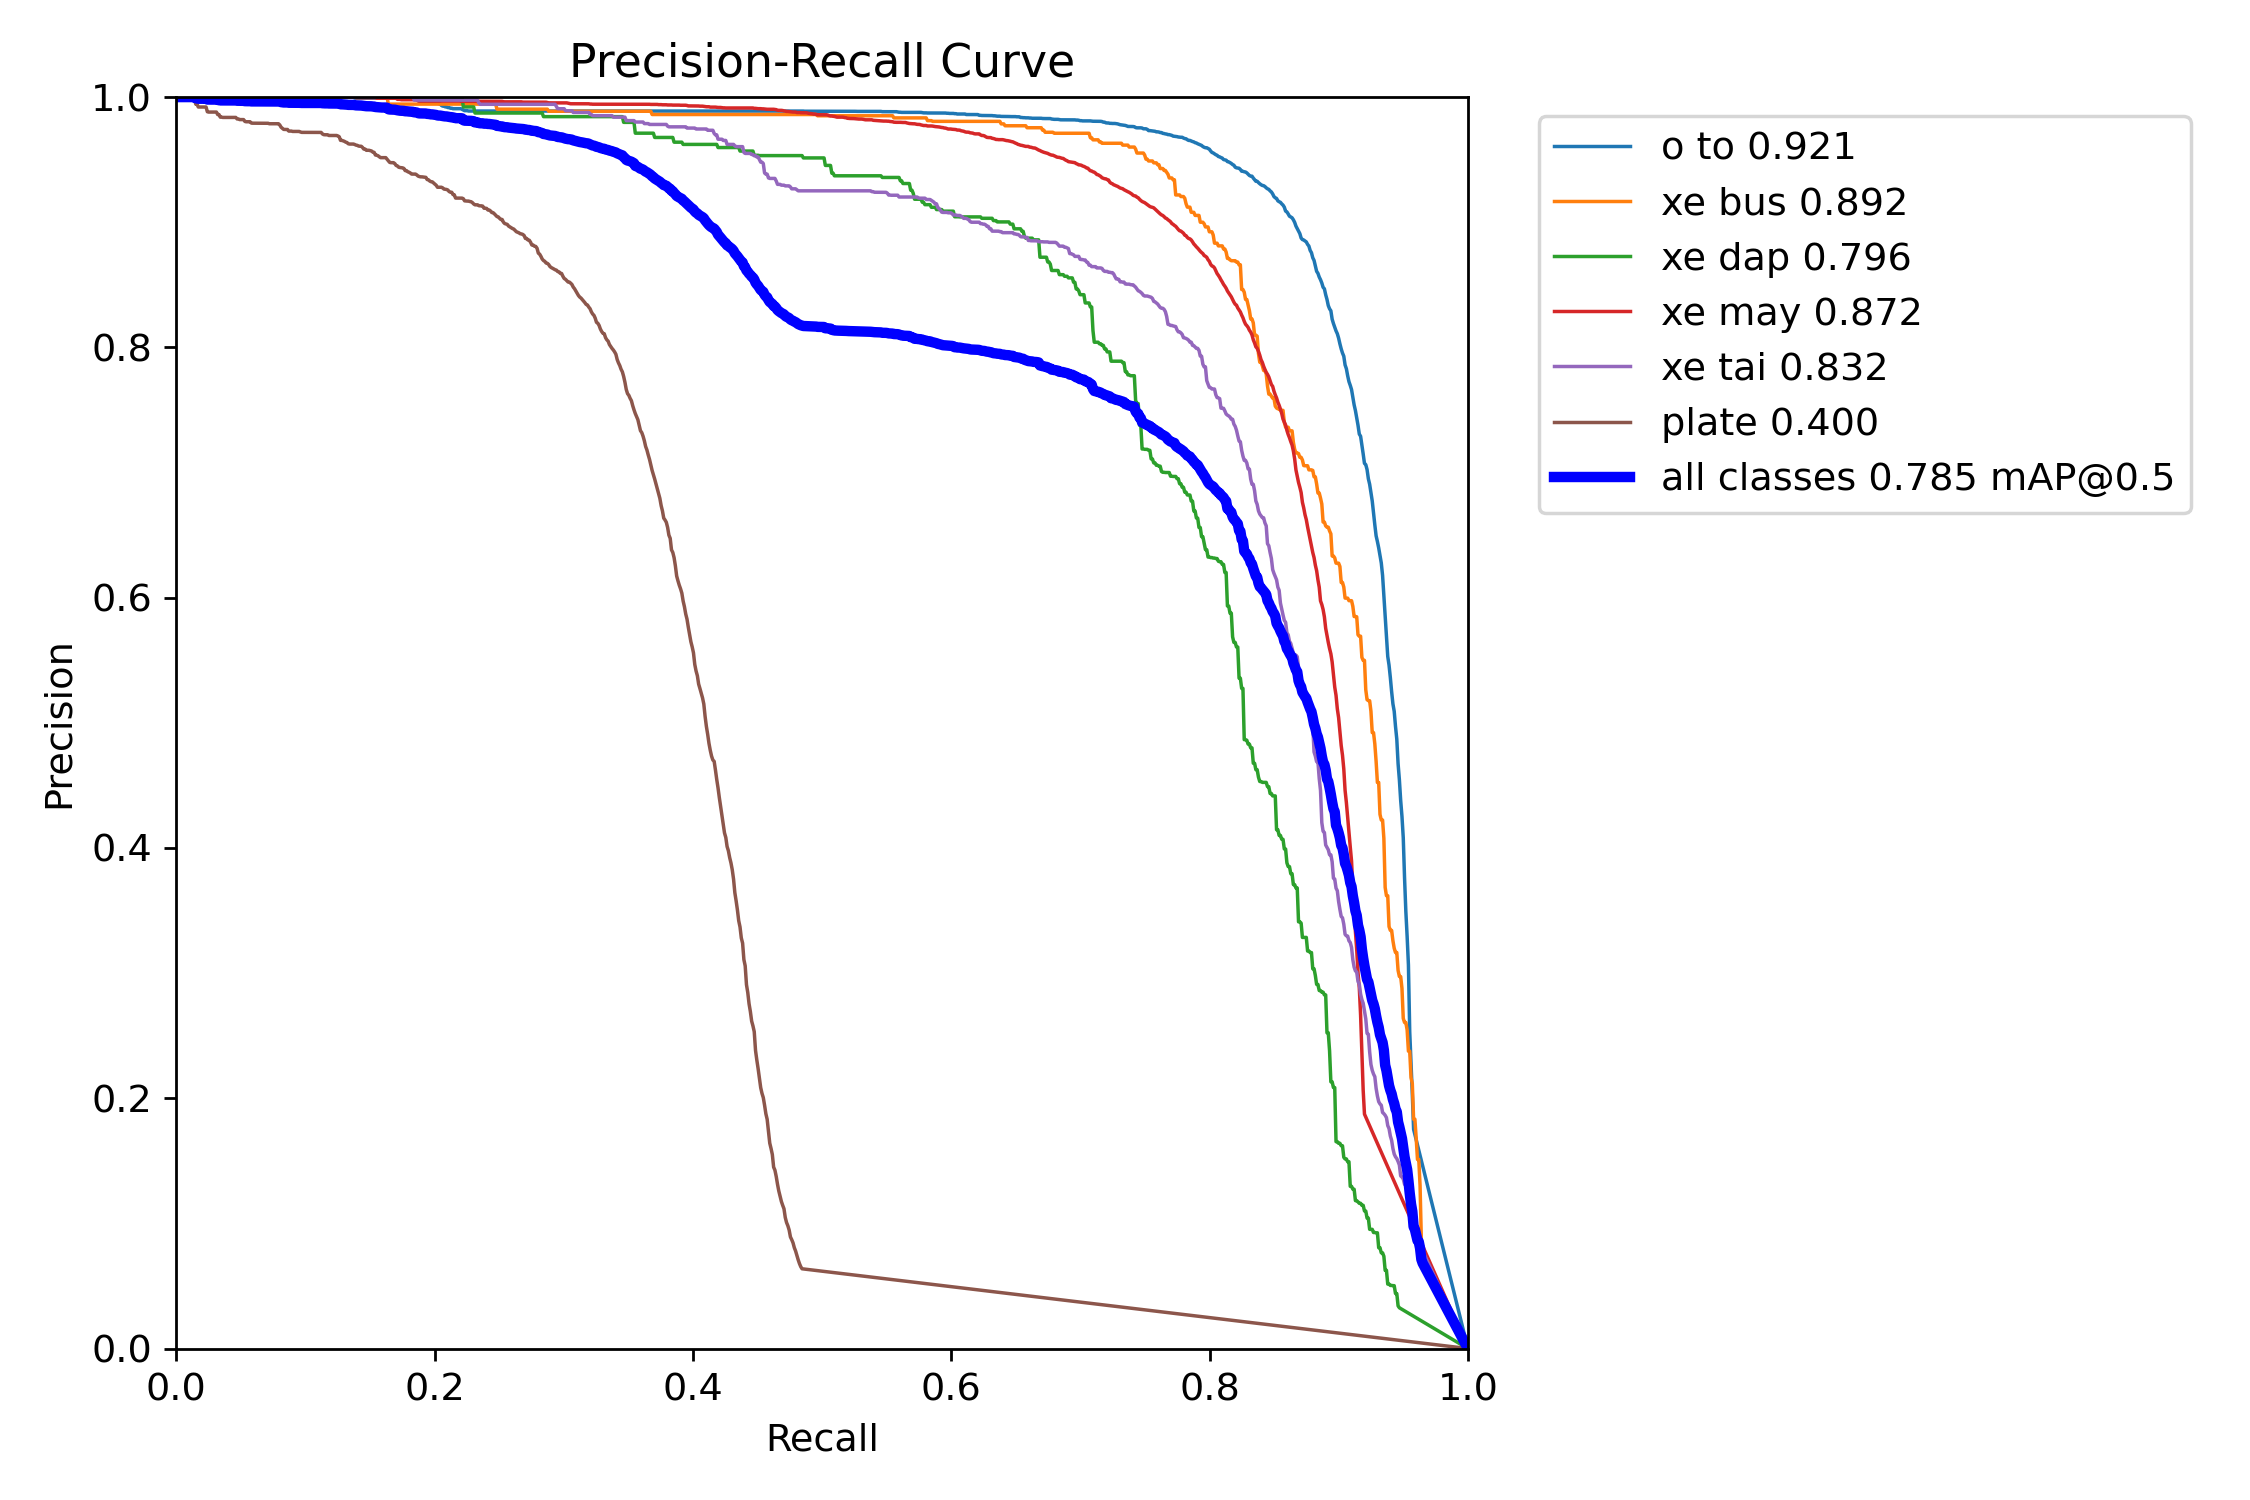
\includegraphics[width=0.8\linewidth]{Figures/multiclass_PR_curve.png}
    \caption{Đường cong Precision-Recall của mô hình tích hợp 6 lớp}
    \label{fig:multiclass_pr_curve}
\end{figure}

\subsection{Kết quả Validation mô hình tích hợp}

\begin{figure}[H]
    \centering
    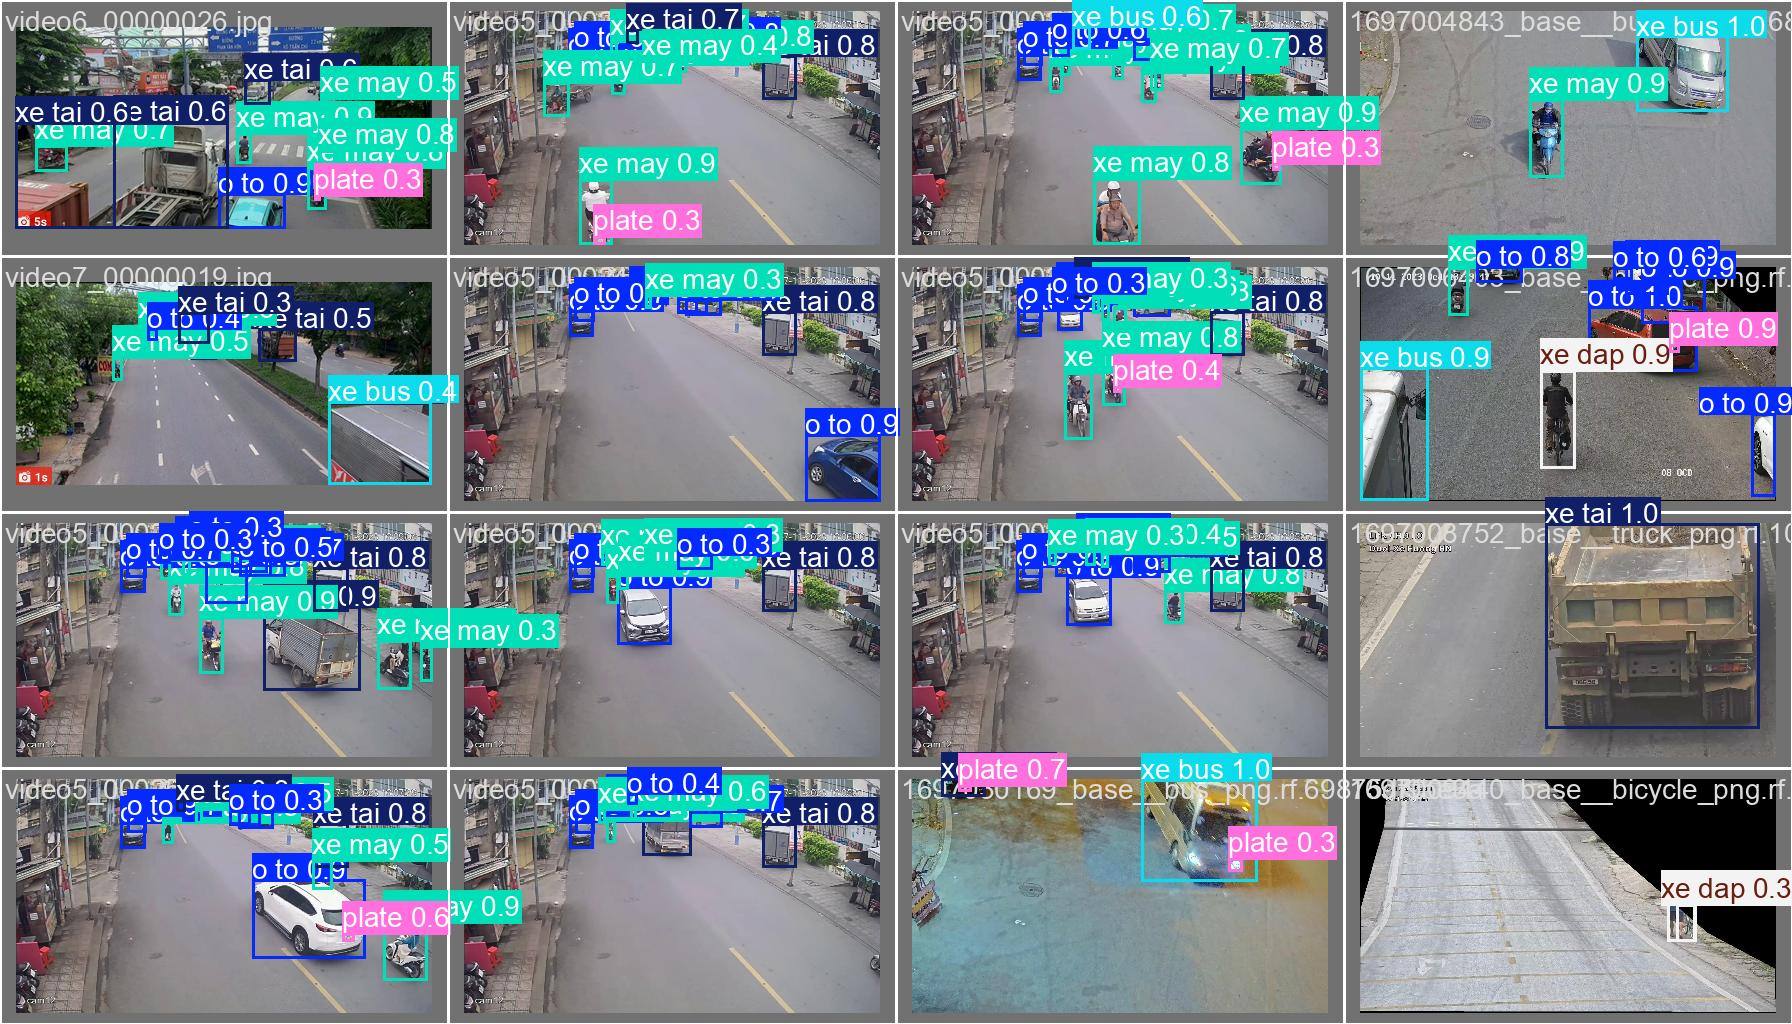
\includegraphics[width=0.95\linewidth]{Figures/multiclass_val_pred.jpg}
    \caption{Kết quả dự đoán trên tập Validation - Mô hình tích hợp 6 lớp (Pipeline 2)}
    \label{fig:multiclass_val_pred}
\end{figure}

Hình \ref{fig:multiclass_val_pred} minh họa kết quả inference của mô hình tích hợp, có thể nhận thấy:
\begin{itemize}
    \item Mô hình phát hiện tốt các loại phương tiện với bounding box chính xác
    \item Biển số được phát hiện khi có kích thước đủ lớn trong khung hình
    \item Một số biển số nhỏ/xa có thể bị bỏ sót (trade-off giữa tốc độ và độ chính xác)
\end{itemize}

%============================================================
% PHẦN 5: KẾT QUẢ INFERENCE THỰC TẾ
%============================================================
\section{Kết quả Inference thực tế}

\subsection{Môi trường thử nghiệm}
Hệ thống được thử nghiệm trên video thực tế tại giao lộ với các điều kiện:
\begin{itemize}
    \item Độ phân giải: 1920 × 1080
    \item FPS video nguồn: 30 FPS
    \item Điều kiện: Ban ngày và ban đêm, nhiều xe qua lại
\end{itemize}

\subsection{Đánh giá Phương pháp 1 (Two-Stage: Model chuyên biệt)}
Kết quả thử nghiệm với mô hình 2 giai đoạn (YOLOv8n phát hiện biển + OCR) cho độ chính xác cao nhưng tốc độ bị giới hạn.

\begin{figure}[H]
    \centering
    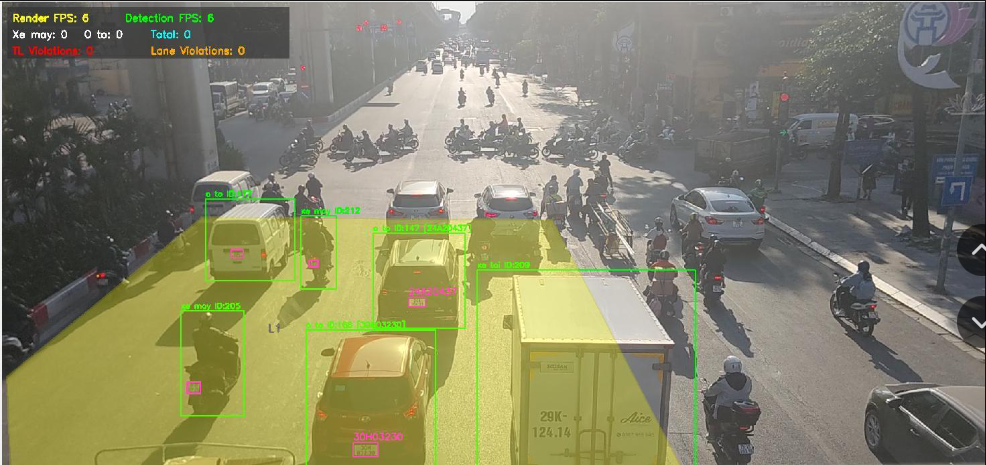
\includegraphics[width=0.9\linewidth]{Figures/plate_inference3.png}
    \caption{Kết quả inference thực tế Phương pháp 1 (Two-Stage)}
    \label{fig:plate_inference_m1}
\end{figure}

\subsubsection{Hiệu năng Phương pháp 1}
\begin{table}[H]
\centering
\caption{Hiệu năng thực tế Phương pháp 1 (Two-Stage)}
\label{tab:perf_m1}
\begin{tabular}{|l|c|}
\hline
\textbf{Chỉ số} & \textbf{Giá trị} \\ \hline
Plate Detection mAP@50 & 99.5\% \\ \hline
Tốc độ xử lý (full pipeline) & 5--10 FPS \\ \hline
Thời gian OCR/biển & ~50ms \\ \hline

\end{tabular}
\end{table}

\subsection{Đánh giá Phương pháp 2 (One-Stage: Model tích hợp)}

Phương pháp 2 sử dụng mô hình tích hợp 6 lớp (5 loại xe + biển số) để phát hiện đồng thời phương tiện và biển số trong một lần forward pass, mang lại tốc độ xử lý nhanh hơn.

\subsubsection{Ưu điểm của Phương pháp 2}
\begin{itemize}
    \item \textbf{Tốc độ cao:} Chỉ cần 1 lần inference qua YOLOv8, đạt 15--20 FPS
    \item \textbf{Mapping tự động:} Dễ dàng liên kết biển số với xe thông qua kiểm tra containment (biển số nằm trong bbox xe)
    \item \textbf{Tiết kiệm tài nguyên:} Chỉ cần load 1 model thay vì 2 models như Phương pháp 1
    \item \textbf{Ngữ cảnh tốt hơn:} Mô hình học được mối quan hệ không gian giữa xe và biển số
\end{itemize}

\subsubsection{Hạn chế của Phương pháp 2}
\begin{itemize}
    \item \textbf{Độ chính xác thấp hơn:} mAP@50 cho biển số chỉ đạt 78.5\% so với 99.5\% của Phương pháp 1
    \item \textbf{Khó phát hiện biển nhỏ:} Do phải cân bằng giữa nhiều lớp, biển số xa hoặc nhỏ dễ bị miss
    \item \textbf{Class imbalance:} Số lượng biển số ít hơn nhiều so với các lớp xe, gây khó khăn trong huấn luyện
\end{itemize}

\subsubsection{Hiệu năng Phương pháp 2}
\begin{table}[H]
\centering
\caption{Hiệu năng thực tế Phương pháp 2 (One-Stage)}
\label{tab:perf_m2}
\begin{tabular}{|l|c|}
\hline
\textbf{Chỉ số} & \textbf{Giá trị} \\ \hline
All Classes mAP@50 & 78.5\% \\ \hline
Tốc độ xử lý (full pipeline) & 15--20 FPS \\ \hline
Số model cần load & 1 (YOLOv8 6-class) \\ \hline
GPU Memory & ~1.2GB \\ \hline
Tỷ lệ mapping thành công & 95\% (containment check) \\ \hline
\end{tabular}
\end{table}

\subsubsection{Kết quả Inference thực tế Phương pháp 2}
Hình \ref{fig:pp2_inference} minh họa kết quả chạy ứng dụng với Phương pháp 2 (One-Stage), cho thấy hệ thống có thể phát hiện đồng thời phương tiện và biển số trong một lần inference.

\begin{figure}[H]
    \centering
    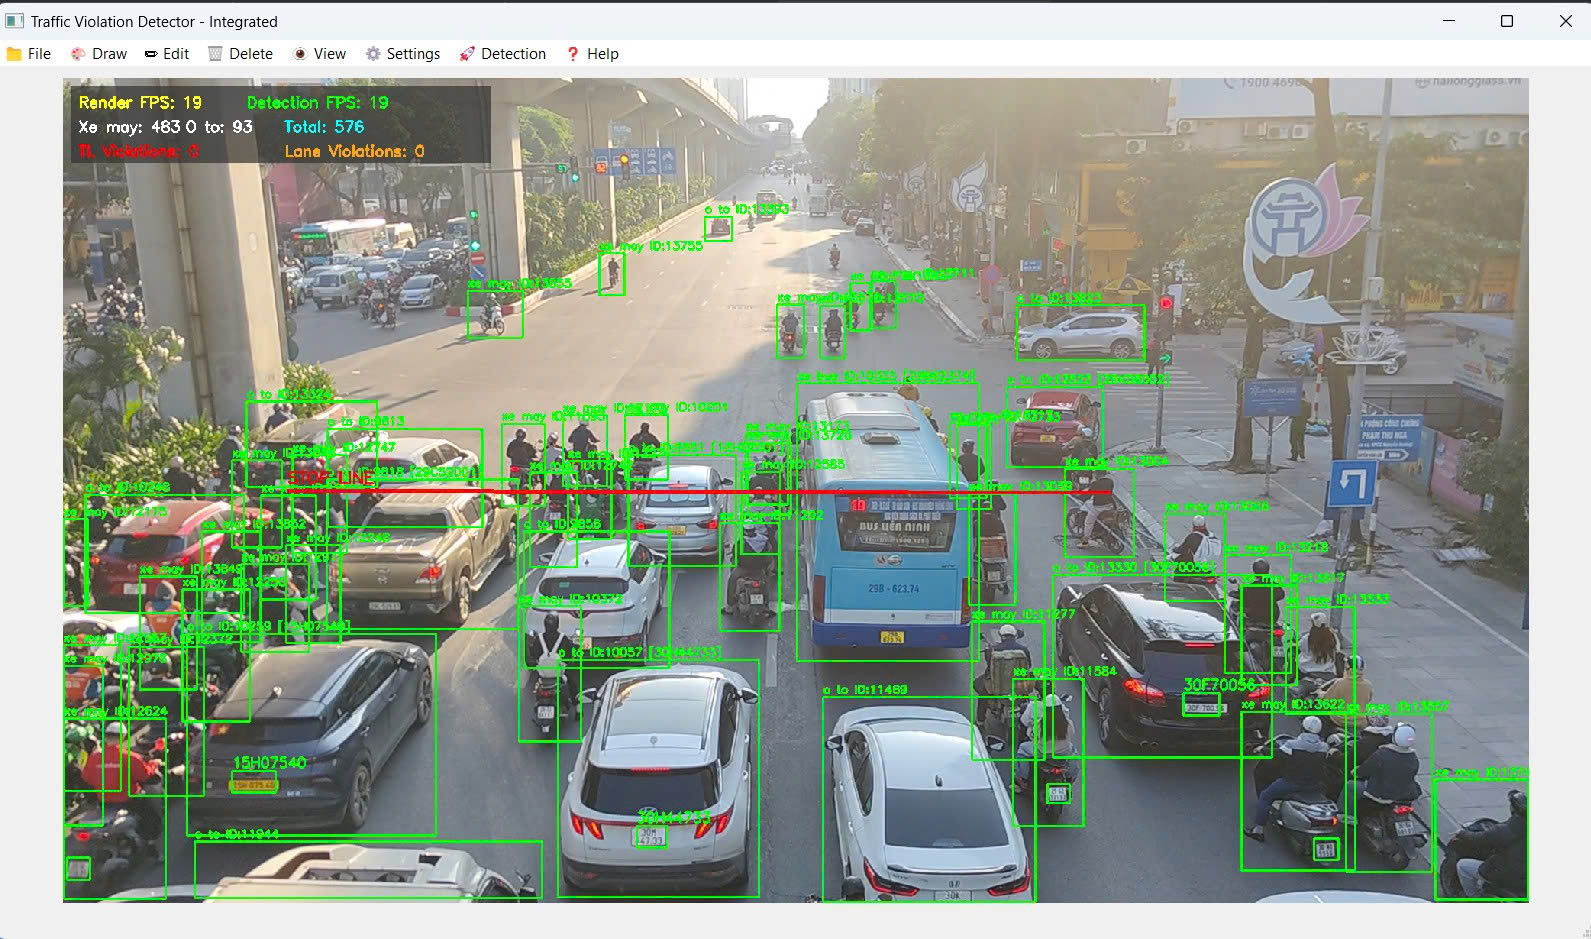
\includegraphics[width=0.95\linewidth]{Figures/ppthucnghiem2.jpg}
    \caption{Kết quả Inference thực tế của Phương pháp 2 (One-Stage: Model tích hợp 6 lớp)}
    \label{fig:pp2_inference}
\end{figure}

\subsection{So sánh hiệu năng hai phương pháp}

%============================================================
% TỔNG HỢP TRỰC QUAN CÁC MODEL
%============================================================
\subsubsection{Tổng hợp trực quan kết quả các Model}

Để có cái nhìn tổng quan, Hình \ref{fig:all_models_summary} trình bày kết quả training của cả 4 thành phần chính trong hệ thống.

\begin{figure}[H]
    \centering
    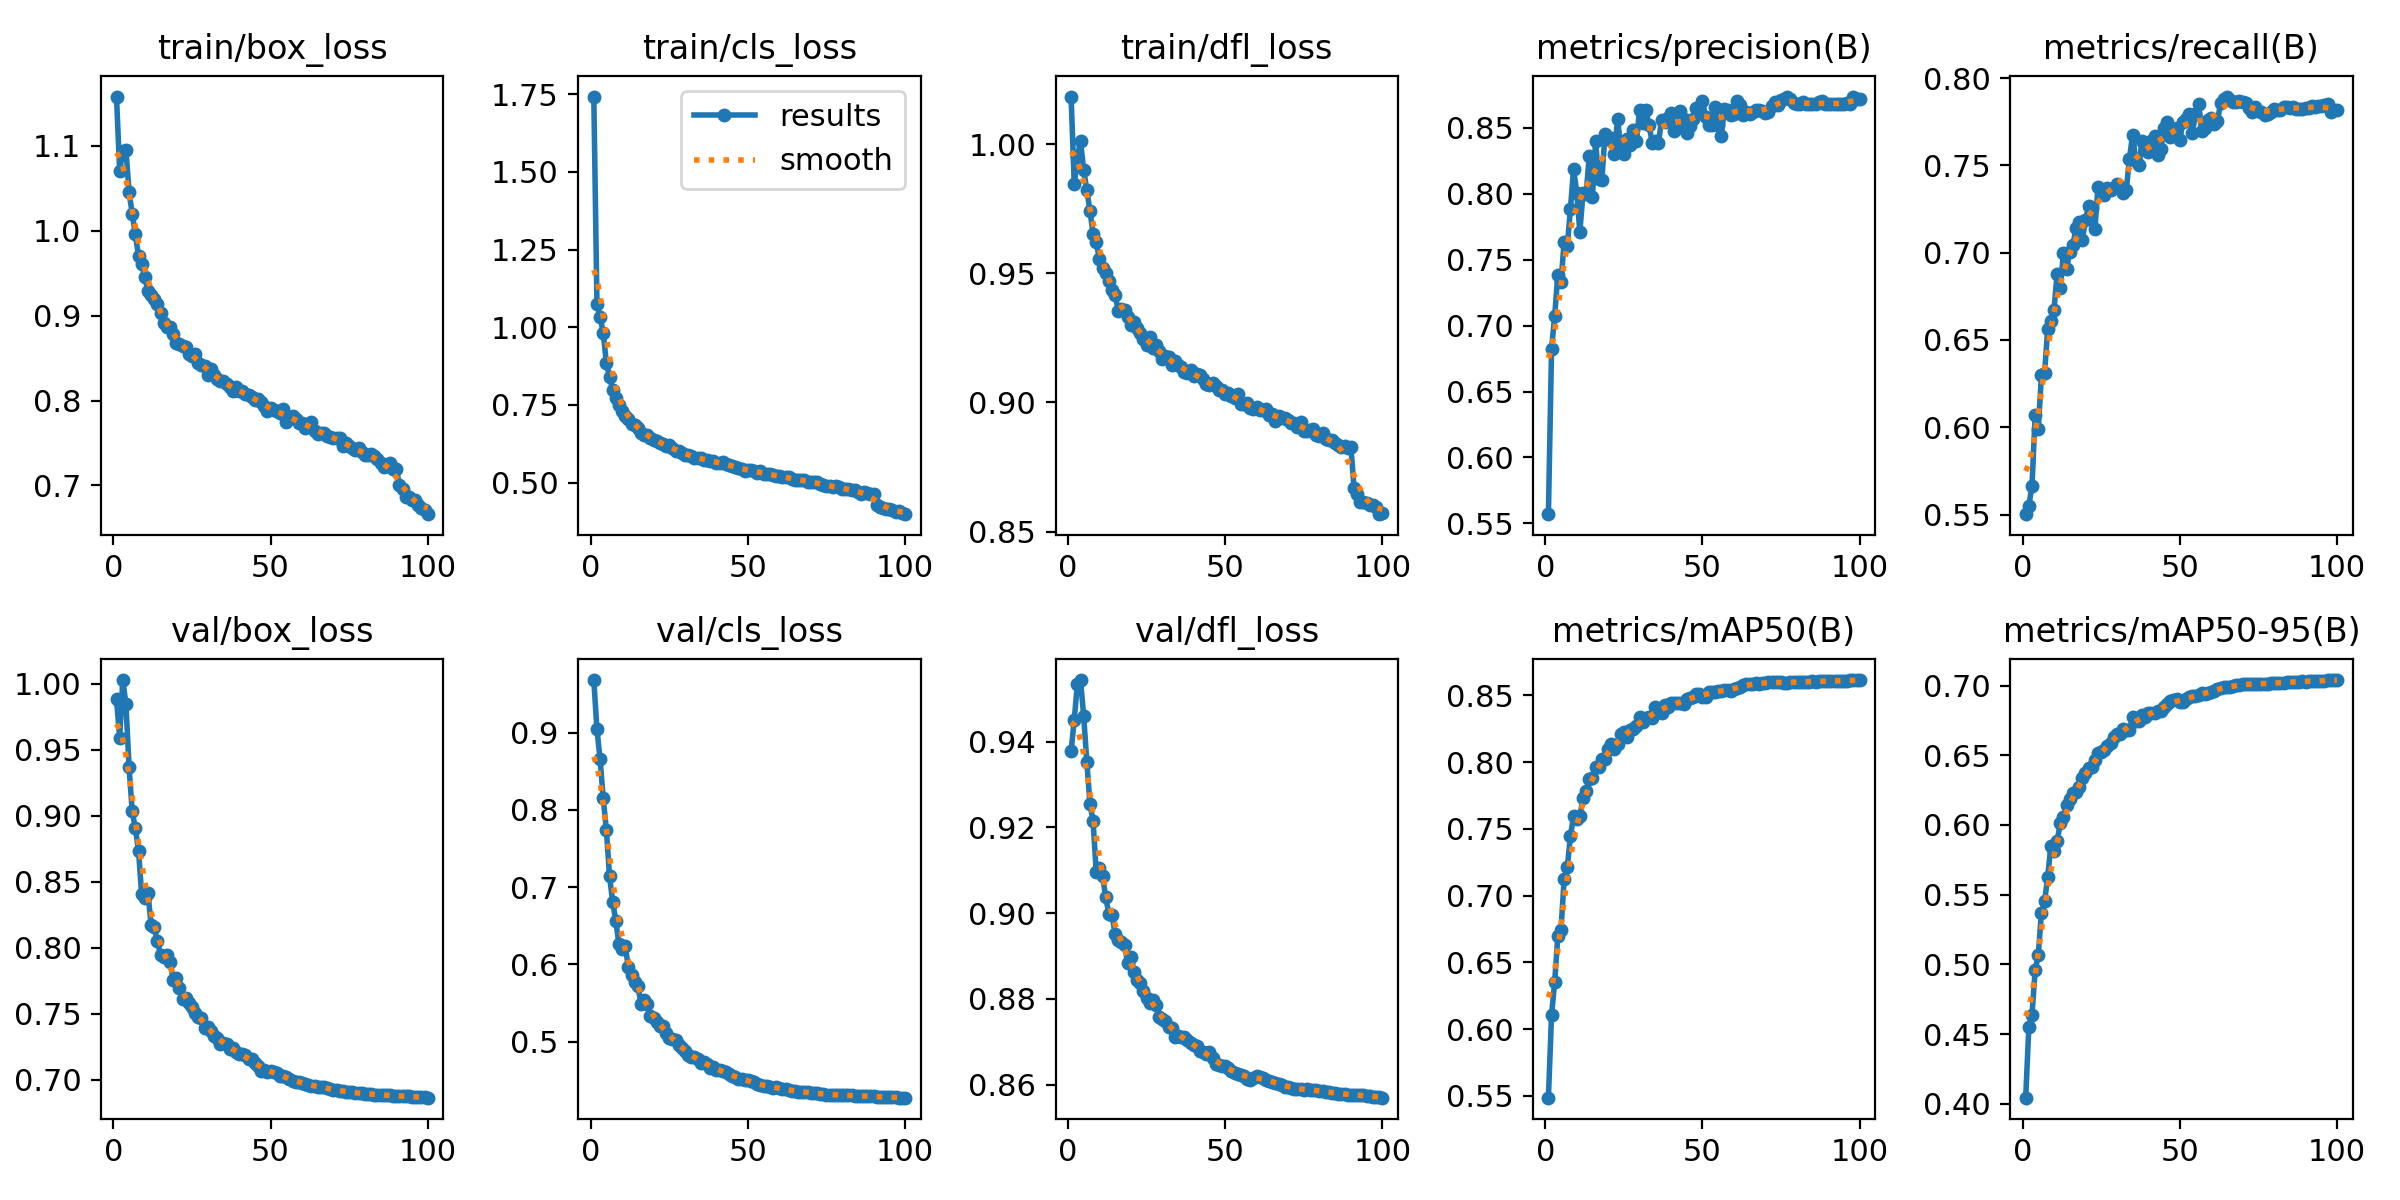
\includegraphics[width=0.85\linewidth]{Figures/results.png}
    \vspace{0.2cm}
    
    (a) Model 1: Phát hiện phương tiện (5 lớp)
    \vspace{0.4cm}
    
    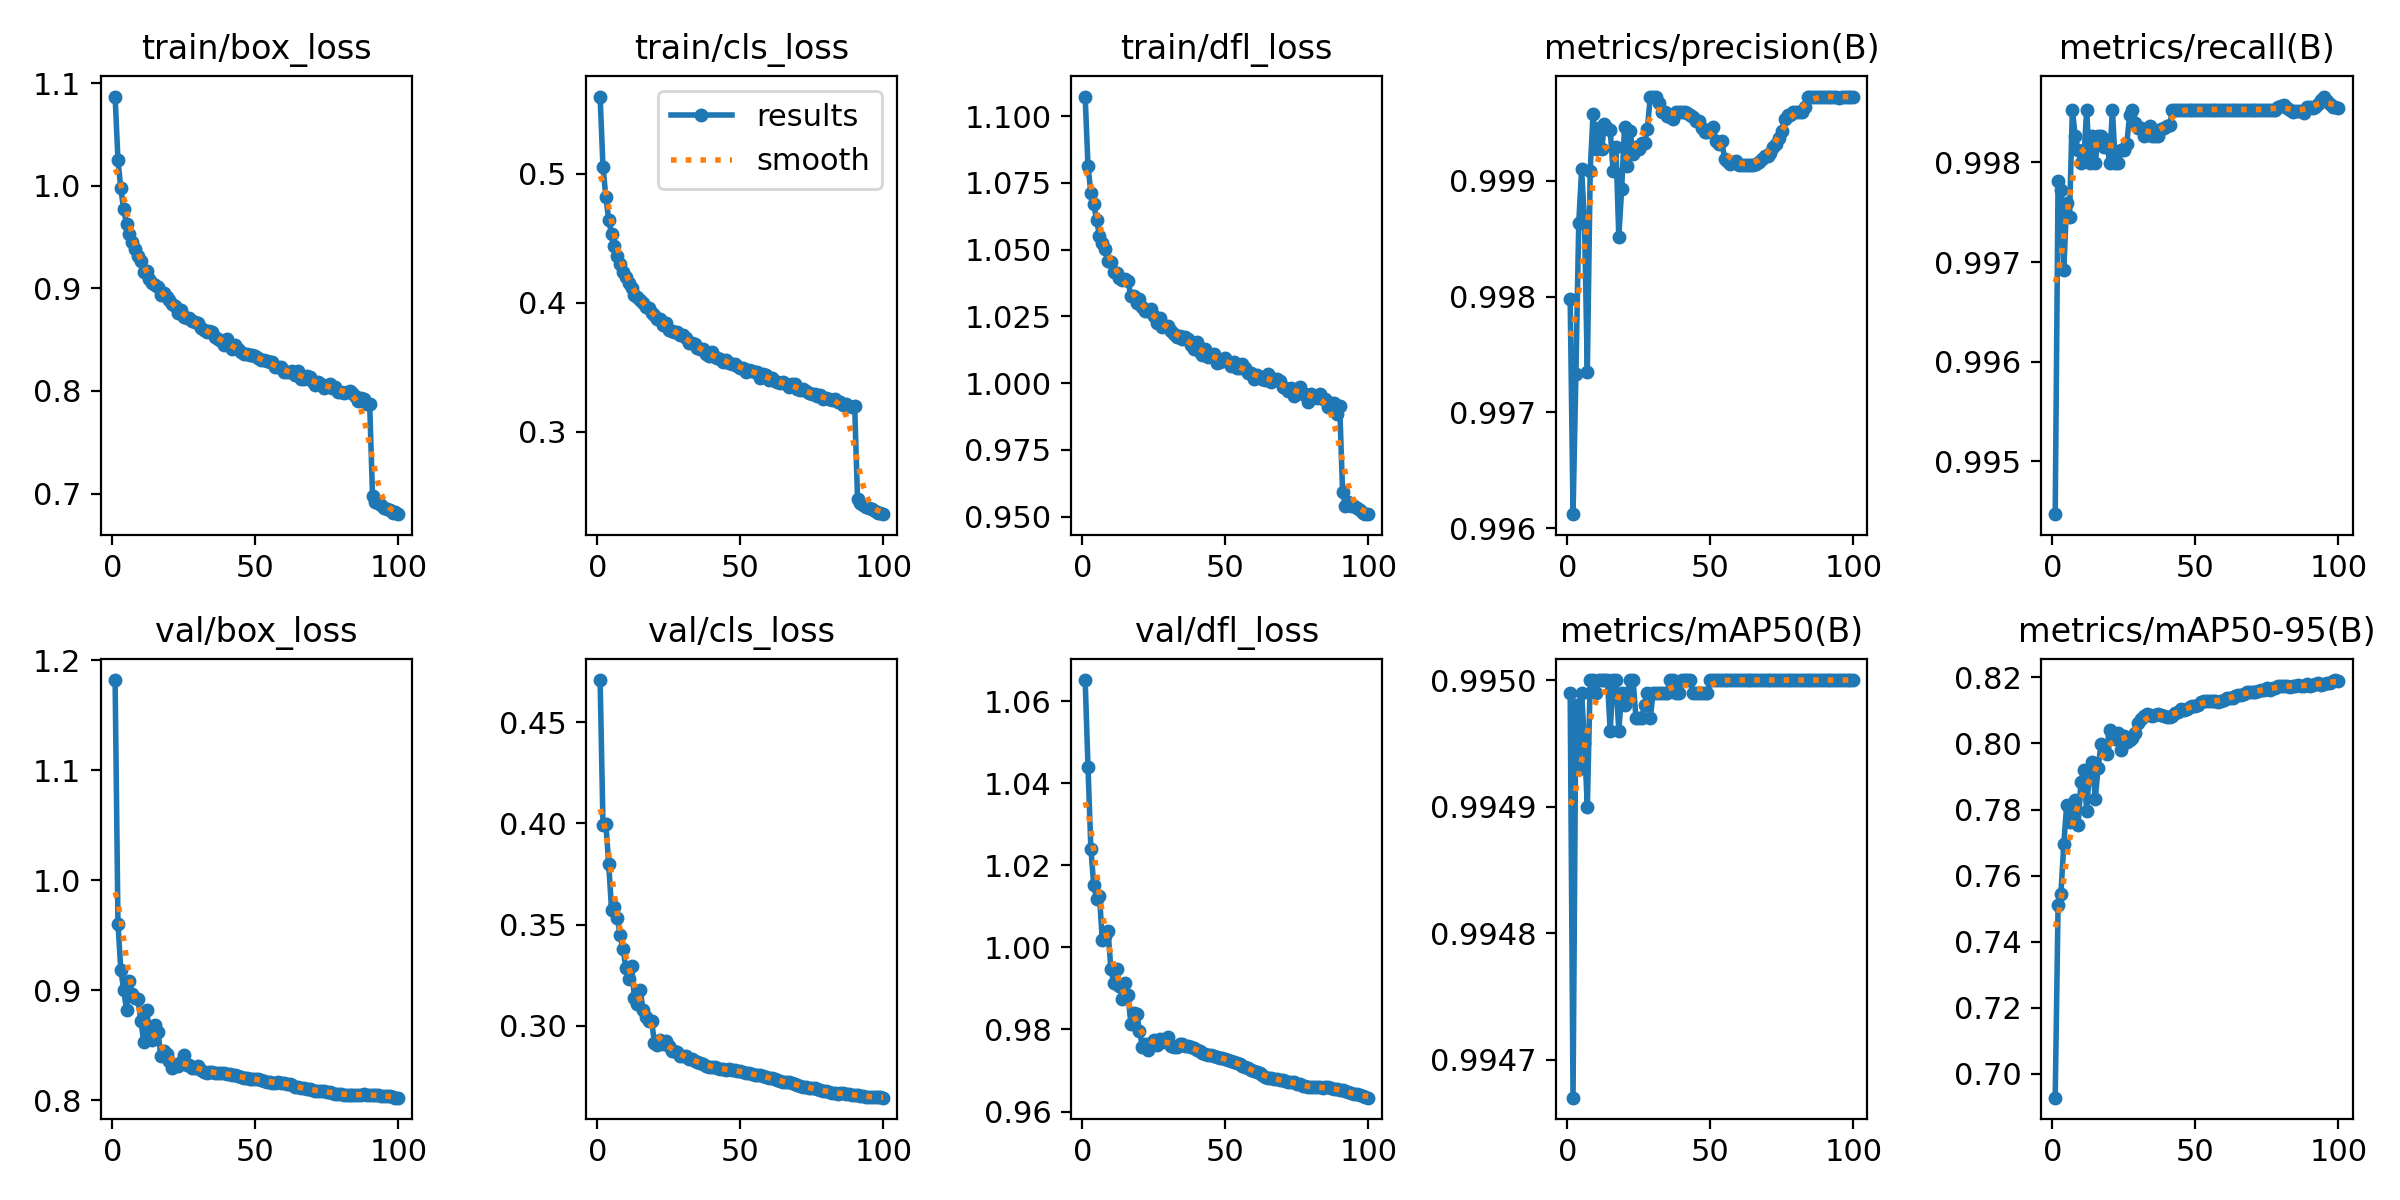
\includegraphics[width=0.85\linewidth]{Figures/plate_results.png}
    \vspace{0.2cm}
    
    (b) Model 2: Phát hiện biển số (1 lớp)
    \vspace{0.4cm}
    
    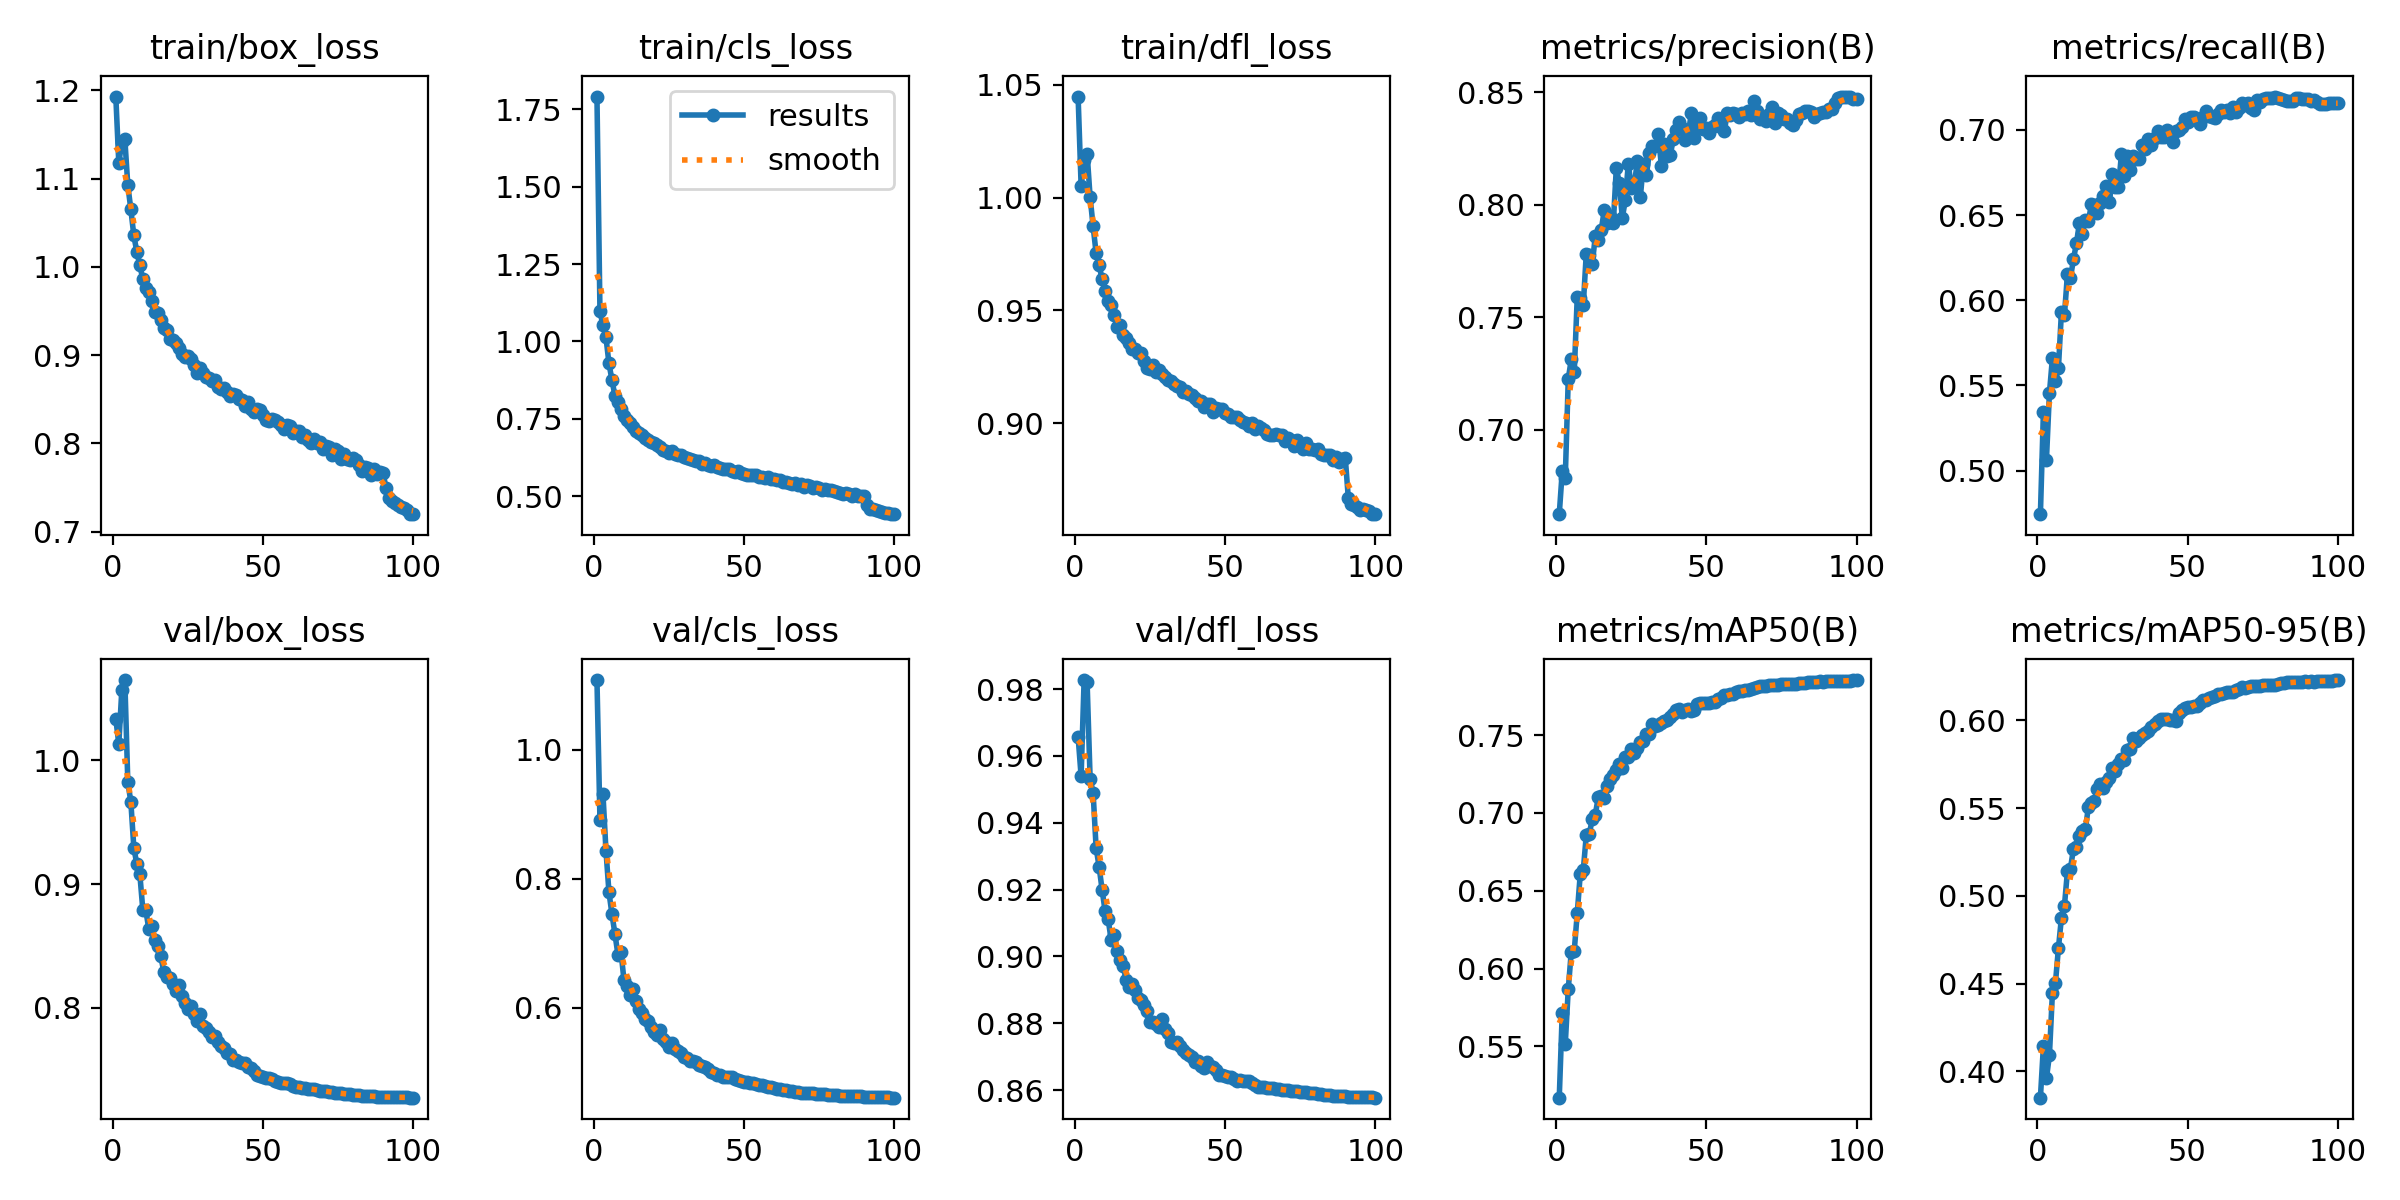
\includegraphics[width=0.85\linewidth]{Figures/multiclass_results.png}
    \vspace{0.2cm}
    
    (c) Mô hình tích hợp 6 lớp (Pipeline 2)
    \caption{Tổng hợp đường cong Loss và Metrics của các model trong hệ thống}
    \label{fig:all_models_summary}
\end{figure}

\begin{figure}[H]
    \centering
    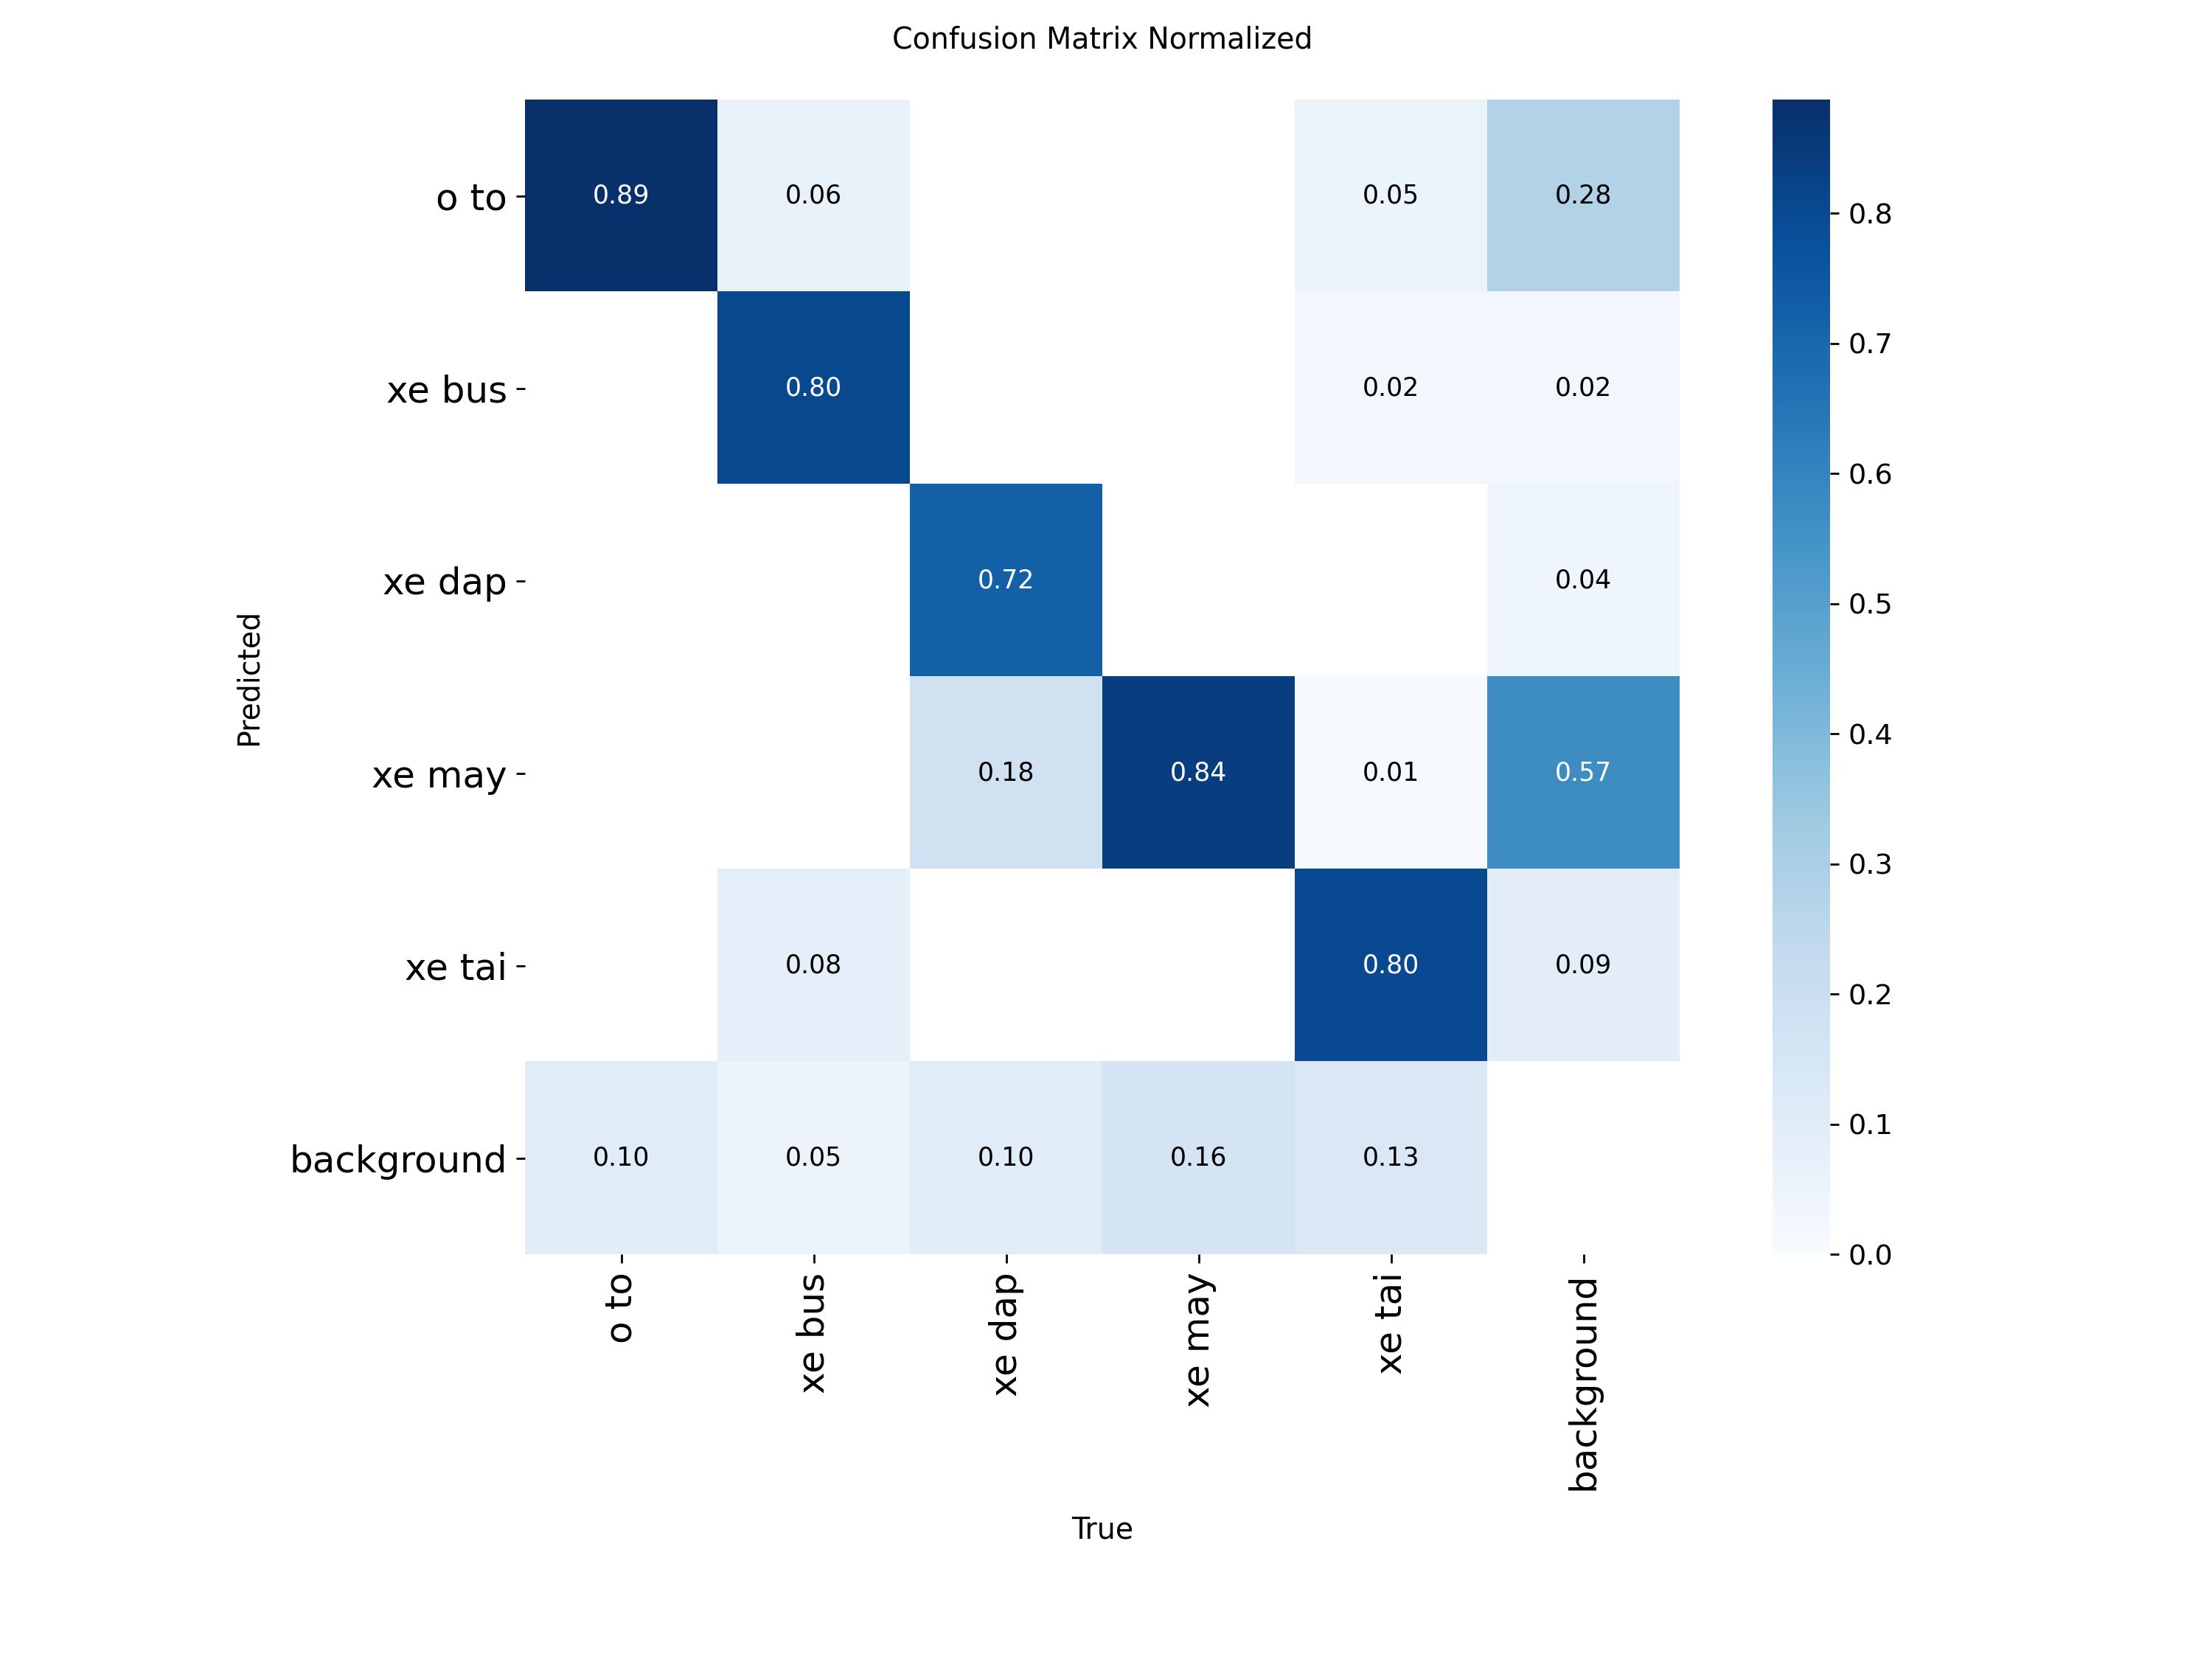
\includegraphics[width=0.65\linewidth]{Figures/confusion_matrix_normalized.png}
    \vspace{0.2cm}
    
    (a) Ma trận nhầm lẫn Model 1 (5 lớp xe)
    \vspace{0.4cm}
    
    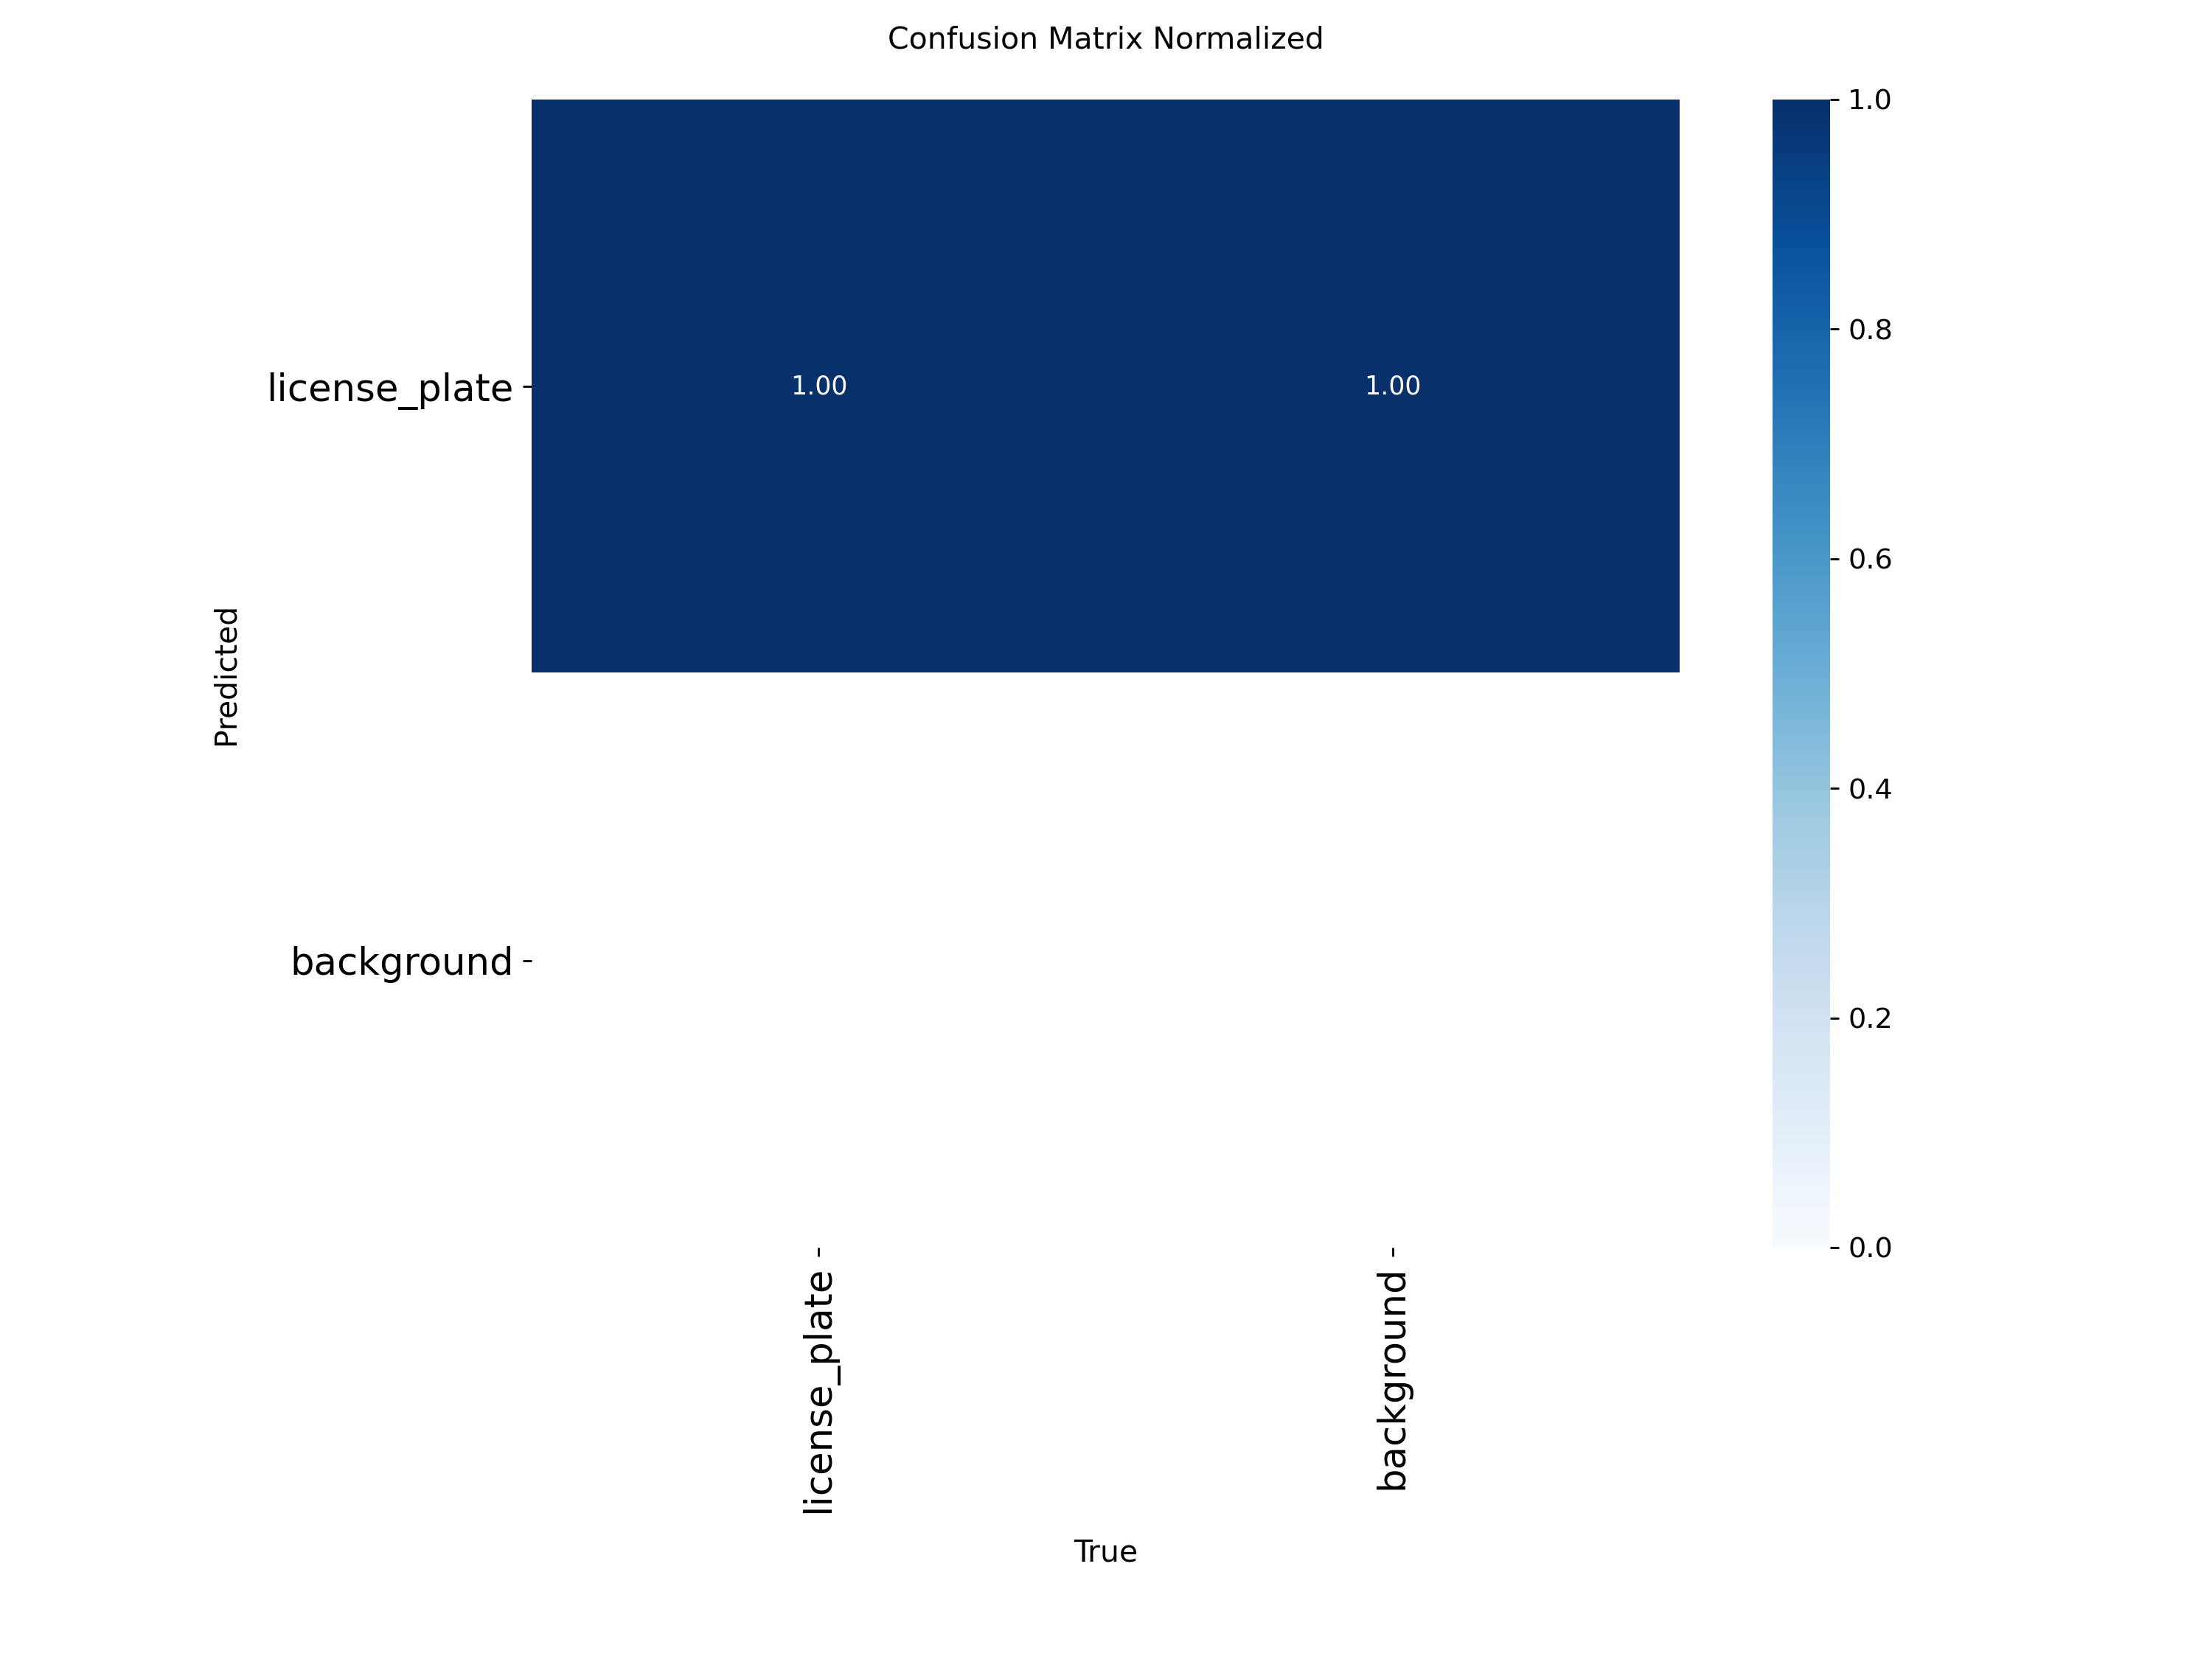
\includegraphics[width=0.65\linewidth]{Figures/plate_confusion_matrix.png}
    \vspace{0.2cm}
    
    (b) Ma trận nhầm lẫn Model 2 (biển số)
    \vspace{0.4cm}
    
    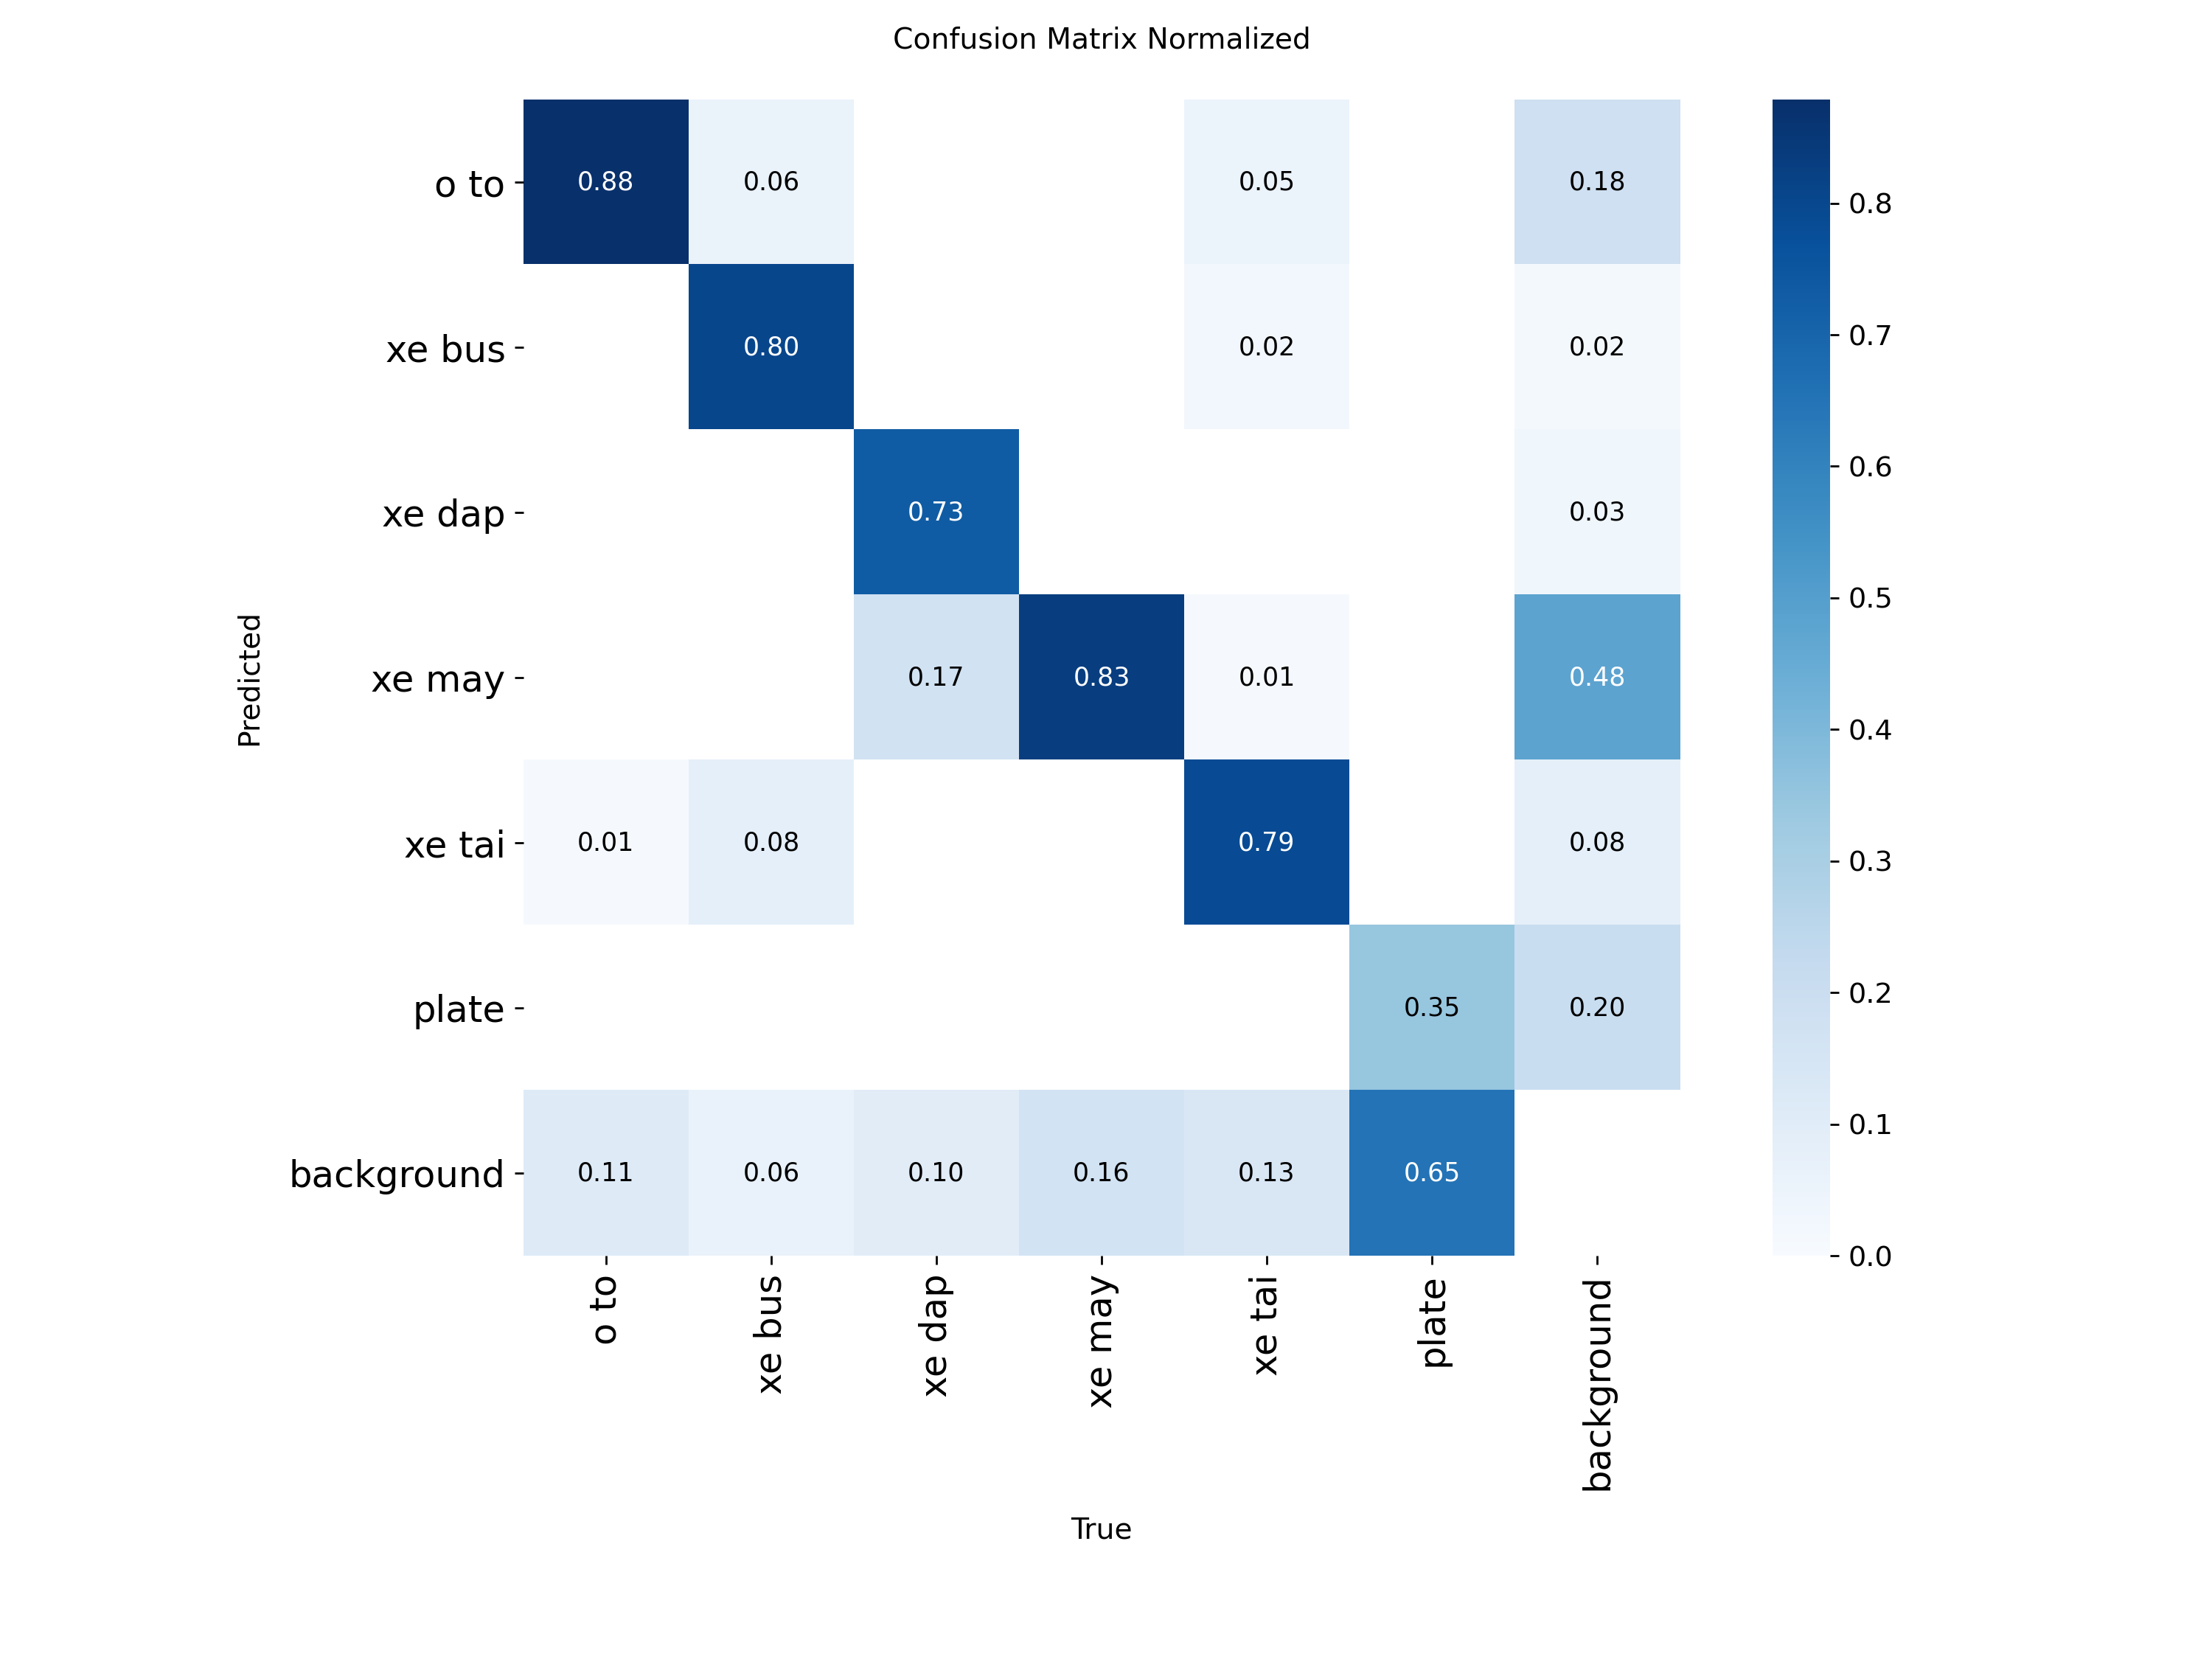
\includegraphics[width=0.65\linewidth]{Figures/multiclass_confusion.png}
    \vspace{0.2cm}
    
    (c) Ma trận nhầm lẫn mô hình tích hợp 6 lớp (Pipeline 2)
    \caption{Tổng hợp ma trận nhầm lẫn của các model trong hệ thống}
    \label{fig:all_confusion_summary}
\end{figure}

\begin{figure}[H]
    \centering
    \begin{tabular}{cc}
        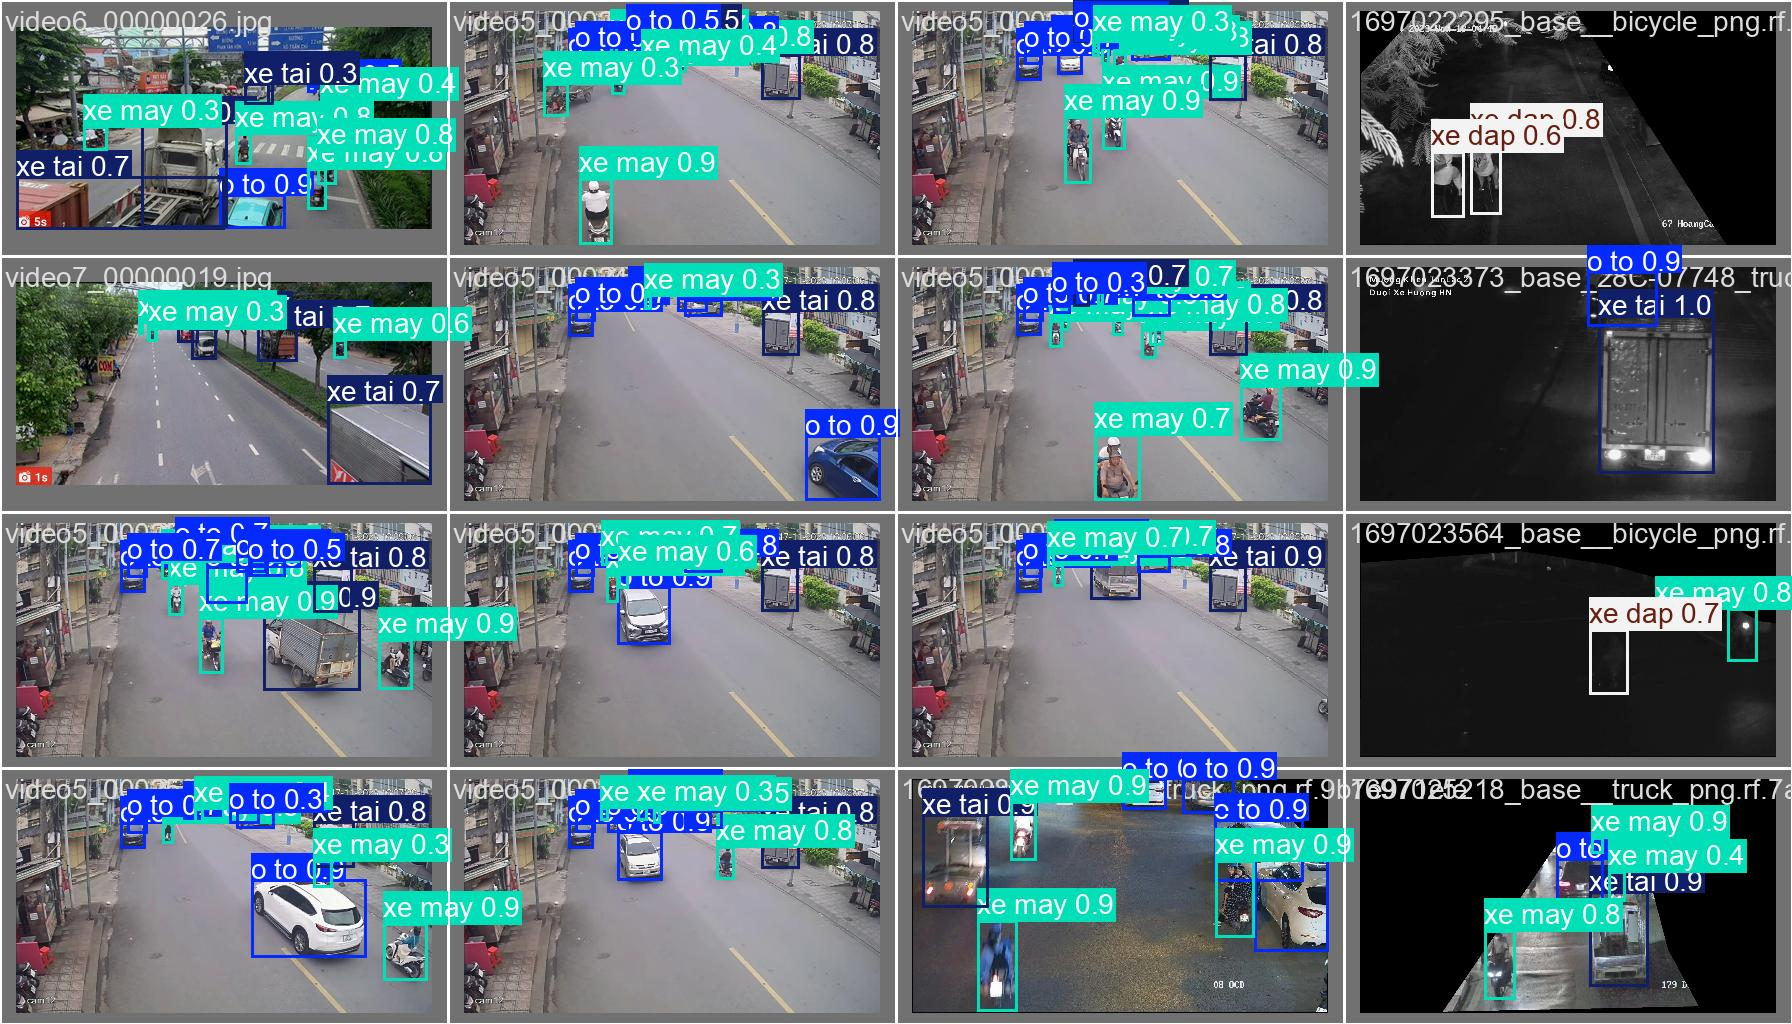
\includegraphics[width=0.48\linewidth]{Figures/val_batch0_pred.jpg} &
        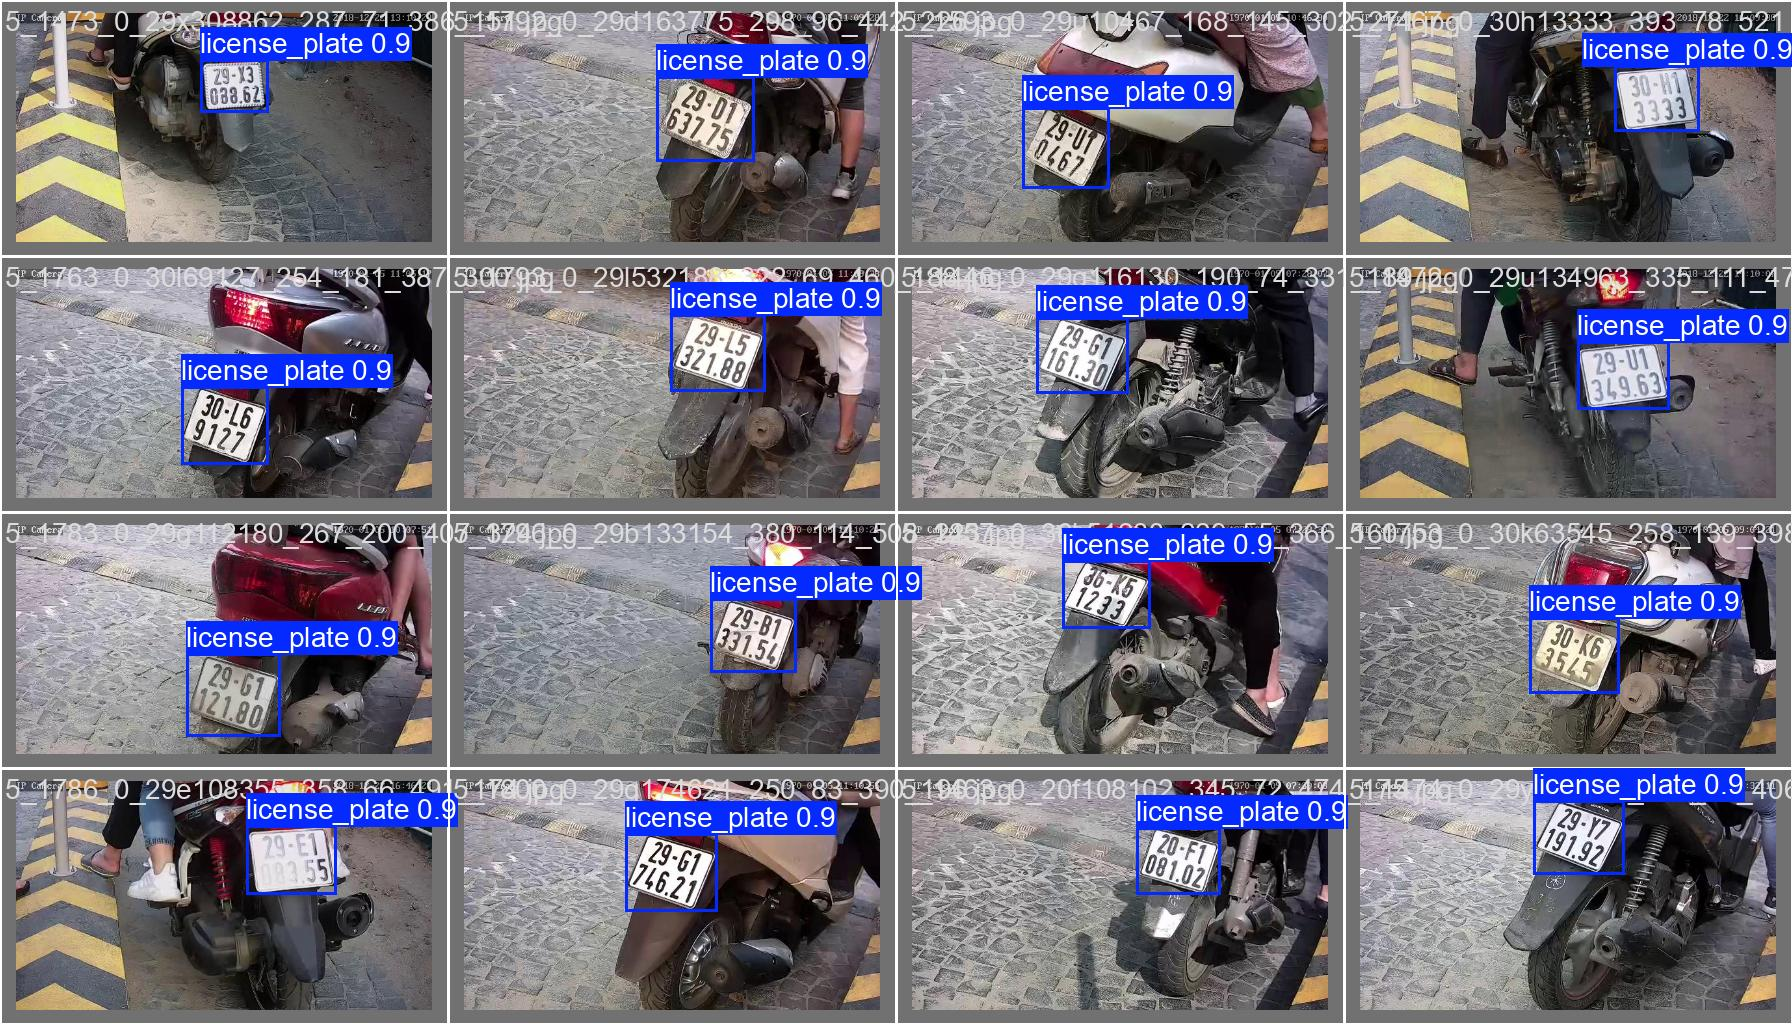
\includegraphics[width=0.48\linewidth]{Figures/plate_val_pred.jpg} \\
        (a) Validation Model 1 (Phát hiện xe) & (b) Validation Model 2 (Phát hiện biển số) \\[0.3cm]
        \multicolumn{2}{c}{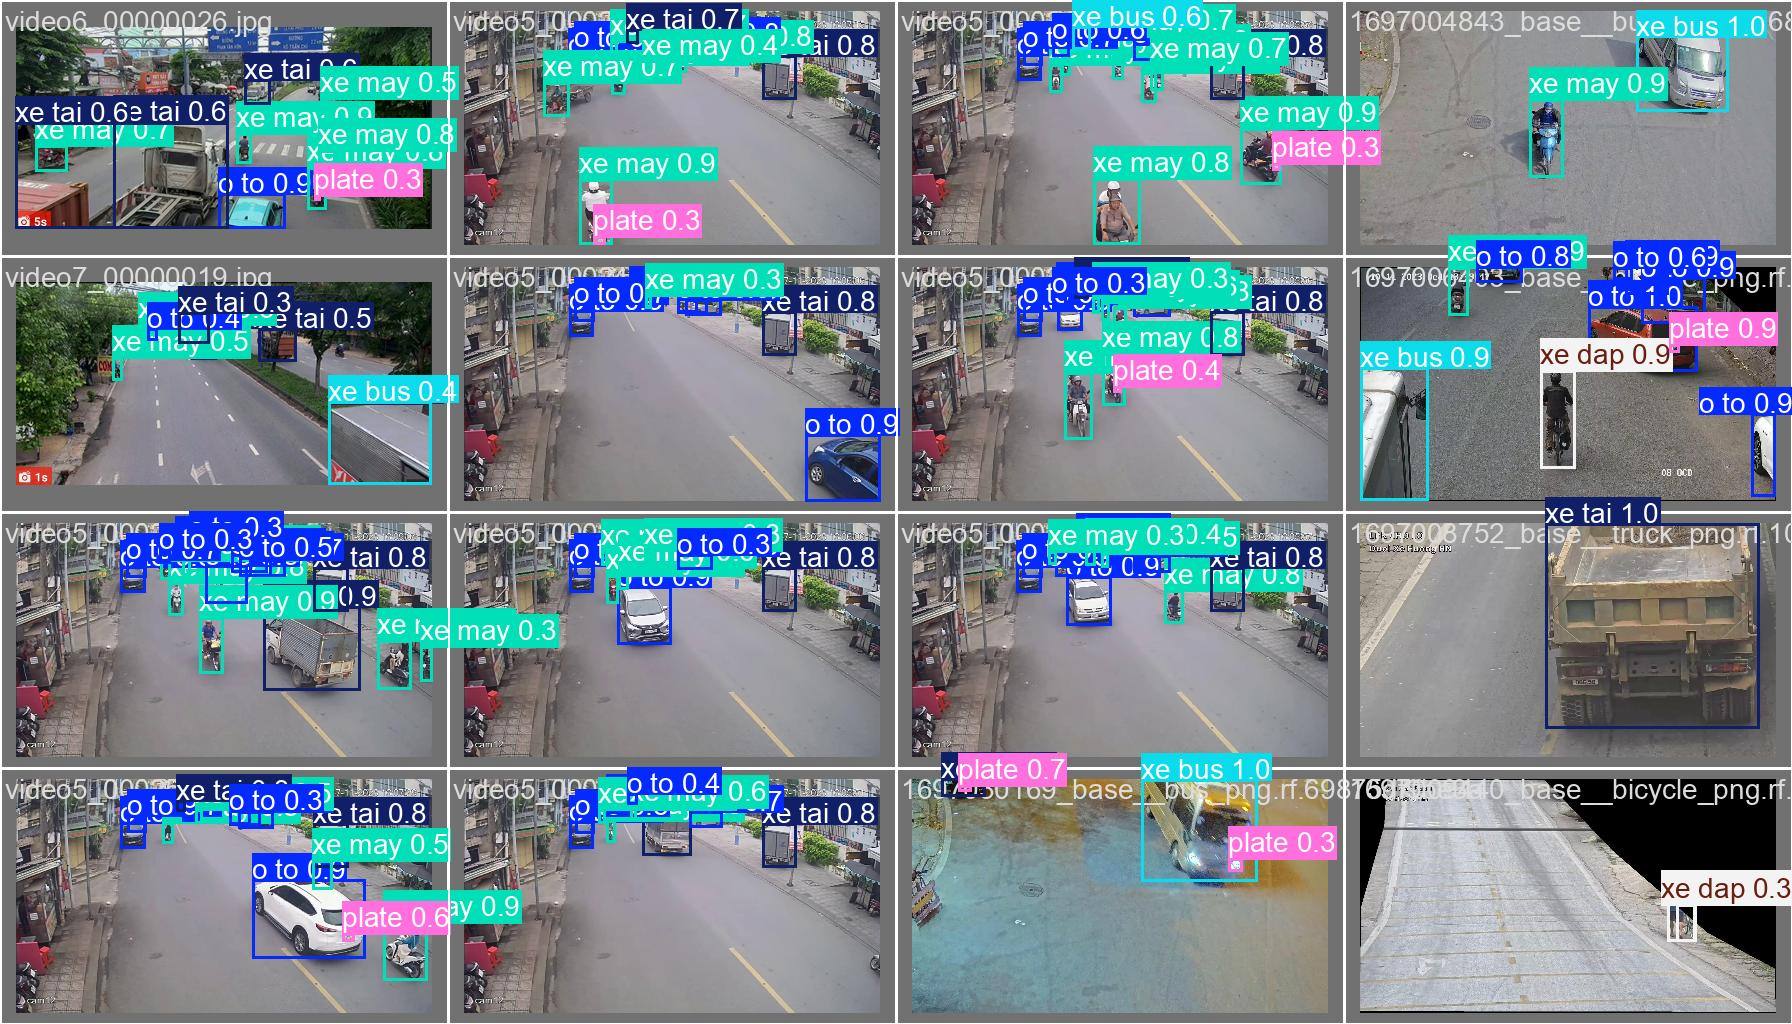
\includegraphics[width=0.7\linewidth]{Figures/multiclass_val_pred.jpg}} \\
        \multicolumn{2}{c}{(c) Validation mô hình tích hợp 6 lớp (xe + biển số)} \\
    \end{tabular}
    \caption{Tổng hợp kết quả Validation của các model trong hệ thống}
    \label{fig:all_val_summary}
\end{figure}

\subsubsection{Bảng so sánh tổng hợp kết quả huấn luyện 3 mô hình}

Bảng \ref{tab:3models_comparison} tổng hợp kết quả huấn luyện của 3 mô hình chính trong hệ thống:

\begin{table}[H]
\centering
\caption{So sánh kết quả huấn luyện 3 mô hình Detection}
\label{tab:3models_comparison}
\begin{tabular}{|l|c|c|c|c|}
\hline
\textbf{Mô hình} & \textbf{Precision} & \textbf{Recall} & \textbf{mAP@50} & \textbf{mAP@50-95} \\ \hline
\textbf{Model 1: Phát hiện phương tiện} & 87.2\% & 78.1\% & 86.1\% & 70.4\% \\ 
\textit{(YOLOv8n, 5 lớp xe, 100 epochs)} & & & & \\ \hline
\textbf{Model 2: Phát hiện biển số} & \textbf{99.97\%} & \textbf{99.86\%} & \textbf{99.50\%} & \textbf{81.90\%} \\ 
\textit{(YOLOv11n, 1 lớp plate, 100 epochs)} & & & & \\ \hline
\textbf{Model tích hợp 6 lớp} & 84.7\% & 71.6\% & 78.5\% & 62.3\% \\ 
\textit{(YOLOv8n, 5 lớp xe + plate, 100 epochs)} & & & & \\ \hline
\end{tabular}
\end{table}

\textbf{Nhận xét:}
\begin{itemize}
    \item \textbf{Model 2 (Phát hiện biển số)} đạt kết quả tốt nhất với mAP@50 = \textbf{99.50\%}, nhờ bài toán đơn lớp và dữ liệu VNLP chất lượng cao.
    \item \textbf{Model 1 (Phát hiện phương tiện)} đạt mAP@50 = \textbf{86.1\%}, phù hợp cho bài toán đa lớp với 5 loại phương tiện khác nhau.
    \item \textbf{Model tích hợp 6 lớp} có mAP@50 thấp hơn (\textbf{78.5\%}) do phải cân bằng giữa nhiều lớp và class imbalance, nhưng mang lại lợi thế về tốc độ xử lý.
\end{itemize}

\subsubsection{So sánh kết quả Inference thực tế giữa hai Pipeline}

\begin{figure}[H]
    \centering
    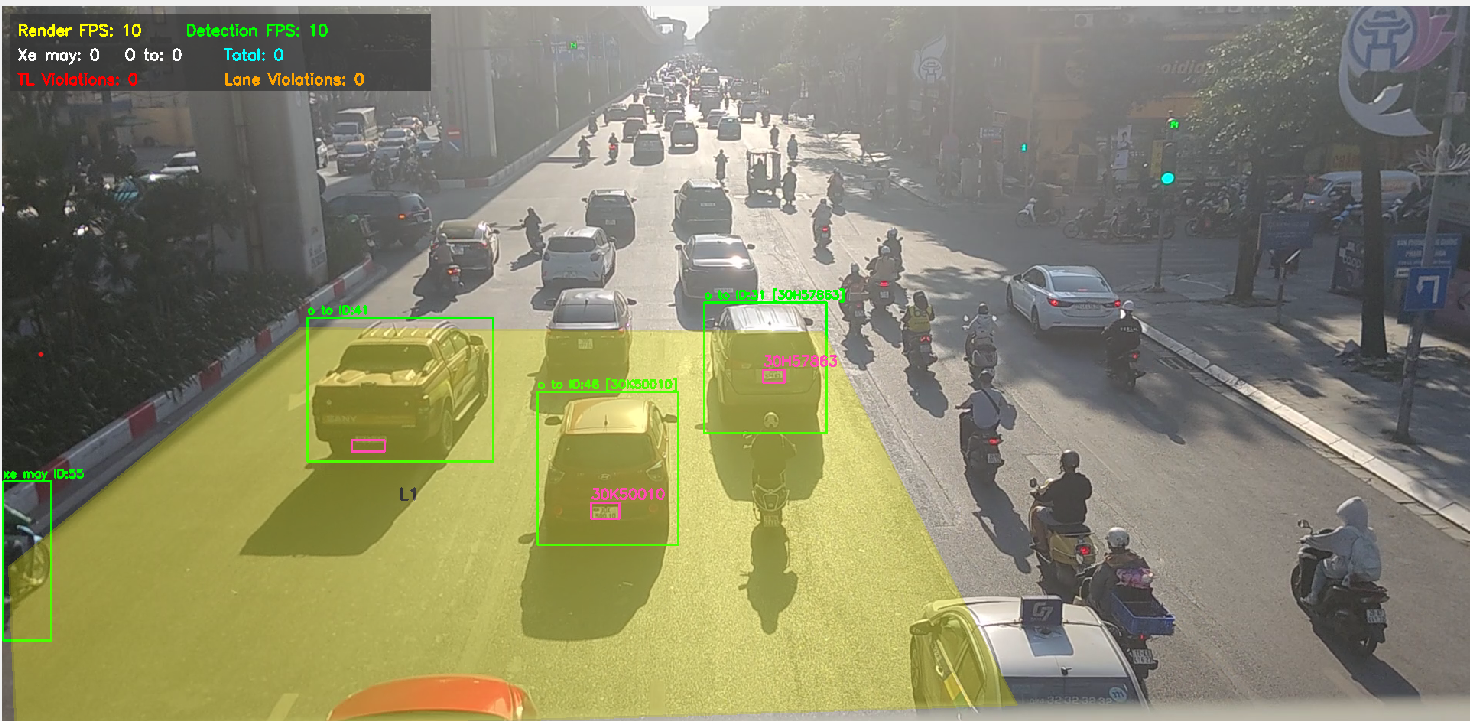
\includegraphics[width=0.9\linewidth]{Figures/plate_inference1.png}
    \caption{Pipeline 1 (Two-Stage): Phát hiện chính xác biển số nhỏ/xa}
    \label{fig:pipeline1_a}
\end{figure}

\begin{figure}[H]
    \centering
    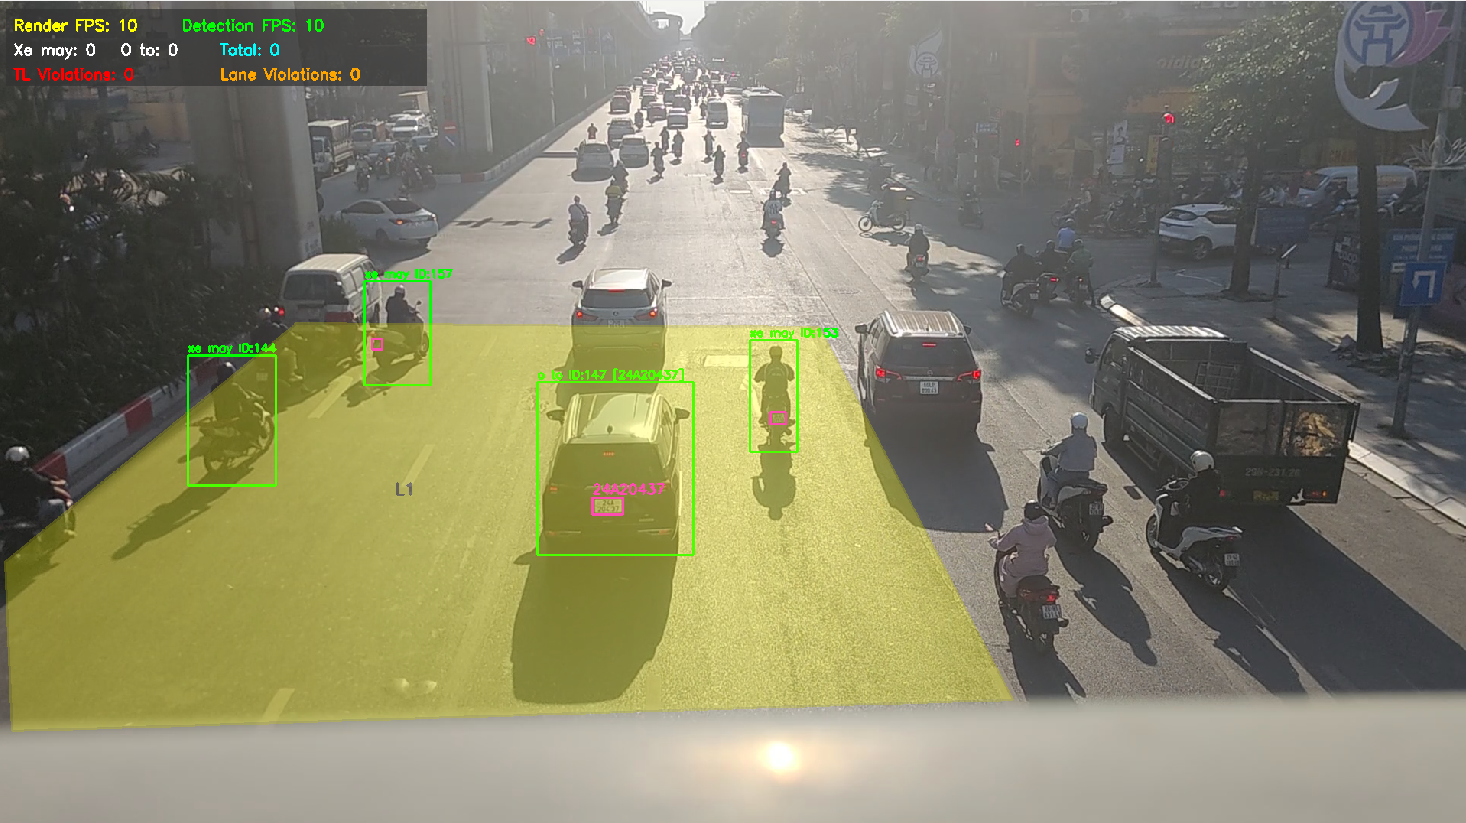
\includegraphics[width=0.9\linewidth]{Figures/plate_inference2.png}
    \caption{Pipeline 1 (Two-Stage): OCR chính xác với biển số rõ nét}
    \label{fig:pipeline1_b}
\end{figure}

\begin{figure}[H]
    \centering
    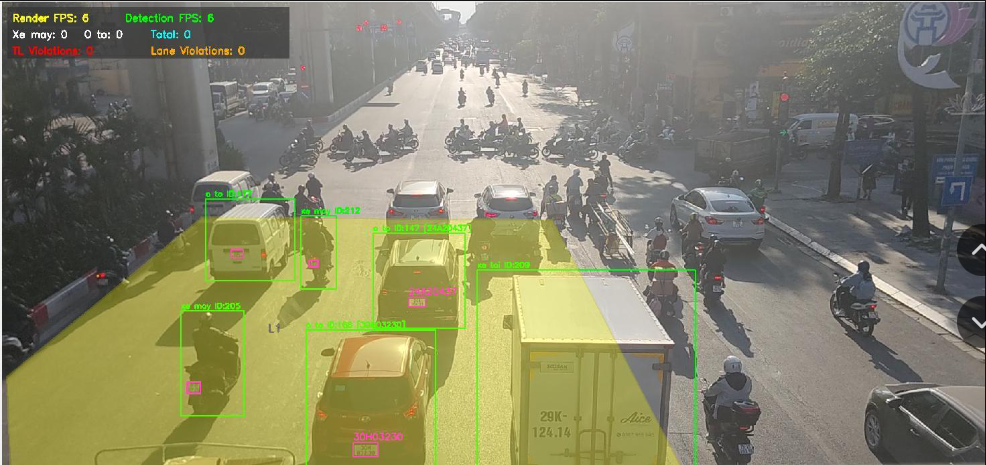
\includegraphics[width=0.9\linewidth]{Figures/plate_inference3.png}
    \caption{Pipeline 1 (Two-Stage): Xử lý tốt nhiều xe trong frame}
    \label{fig:pipeline1_c}
\end{figure}

\textbf{Nhận xét Pipeline 1:}
\begin{itemize}
    \item Phát hiện được hầu hết biển số trong frame, kể cả biển nhỏ/xa
    \item OCR cho kết quả chính xác với định dạng biển số Việt Nam
    \item Tốc độ chậm hơn (5-10 FPS) do cần 2 lần inference
\end{itemize}

\subsubsection{Bảng so sánh định lượng}
\begin{table}[H]
\centering
\caption{Bảng so sánh hiệu năng hai phương pháp phát hiện biển số}
\label{tab:method_comparison}
\begin{tabular}{|l|c|c|}
\hline
\textbf{Tiêu chí} & \textbf{Phương pháp 1 (Two-Stage)} & \textbf{Phương pháp 2 (One-Stage)} \\ \hline
FPS trung bình & 5--10 FPS & 15--20 FPS \\ \hline
Khả năng nhận diện nhỏ & tốt & Trung bình \\ \hline
Tài nguyên tiêu thụ & Cao (2 model) & Thấp (1 model) \\ \hline
Độ phức tạp triển khai & Cao & Thấp \\ \hline

GPU Memory & ~2.5GB & ~1.2GB \\ \hline
\end{tabular}
\end{table}

\subsubsection{Khuyến nghị sử dụng}
\begin{itemize}
    \item \textbf{Phương pháp 1 (Two-Stage):} Phù hợp khi yêu cầu độ chính xác cao, camera có độ phân giải tốt, biển số nhỏ hoặc xa
    \item \textbf{Phương pháp 2 (One-Stage):} Phù hợp khi ưu tiên tốc độ xử lý real-time, tài nguyên hạn chế, biển số đủ lớn trong khung hình
\end{itemize}

%============================================================
% PHẦN 6: ĐÁNH GIÁ HỆ THỐNG PHÁT HIỆN VI PHẠM
%============================================================
\section{Đánh giá hệ thống phát hiện vi phạm}

Dựa trên kết quả thử nghiệm trên hai tình huống vi phạm điển hình: (1) Dừng đè vạch khi đèn đỏ và (2) Xe máy đi vào làn đường ô tô, hệ thống đã cho thấy hiệu quả hoạt động khả quan.

\subsection{Phân tích kết quả nhận diện}

\subsubsection{Tính chính xác của Logic}
\begin{itemize}
    \item \textbf{Trường hợp dừng đèn đỏ (Bbox Đỏ vs Xanh):}
    \begin{itemize}
        \item \textit{Nhóm vi phạm:} Hệ thống đã đánh dấu chính xác nhóm xe máy ở hàng đầu tiên bằng Bbox màu đỏ. Quan sát thực tế cho thấy bánh trước của những xe này đã vượt qua hoặc chạm vào vạch dừng màu trắng, đúng với quy tắc xử lý vi phạm.
        \item \textit{Nhóm tuân thủ:} Các xe được đóng khung màu xanh, không vi phạm phù hợp với tín hiệu đèn. Điều này xác nhận thuật toán so sánh tọa độ Bbox với vạch kẻ đang hoạt động ổn định.
    \end{itemize}

    \item \textbf{Trường hợp đi sai làn:}
    \begin{itemize}
        \item \textit{Nhận diện ngữ cảnh:} Trên mặt đường gồm các ô màu vàng được chia, xác định đây là làn dành riêng được cài đặt trước.
        \item \textit{Phát hiện vi phạm:} Hệ thống phát hiện được xe máy đi lọt lòng vào giữa làn đường này. Mặc dù góc quay thấp và xe bị che khuất một phần, logic vẫn định vị đúng đối tượng nằm trong vùng cấm.
    \end{itemize}
\end{itemize}

\subsubsection{Khả năng phát hiện vật thể}
\begin{itemize}
    \item \textbf{Mật độ và kích thước:}
    \begin{itemize}
        \item Mật độ nhận diện dày đặc, ít có hiện tượng bỏ sót ngay cả với các xe nằm khuất phía sau hoặc ở xa.
    \end{itemize}
\end{itemize}

\subsection{Đánh giá về thách thức môi trường}
\begin{itemize}
    \item \textbf{Ánh sáng và lóa:} Hình ảnh ban đêm có độ tương phản cao và lóa sáng từ đèn xe. Việc Bbox vẫn ôm sát đối tượng chứng tỏ dữ liệu huấn luyện đa dạng (bao gồm mẫu ban đêm) và các kỹ thuật Augmentation (như Random HSV, Mosaic) đã phát huy tác dụng tốt.

    \item \textbf{Cơ sở hạ tầng (Vạch kẻ đường):}
    \begin{itemize}
        \item \textit{Vạch mờ:} Tại ngã tư, vạch dừng trắng khá mờ và cũ. Nếu hệ thống dùng Lane Detection tự động thì đây là thách thức lớn, nhưng nếu dùng vùng quan sát cố định (ROI) thì kết quả cho thấy sự ổn định.
        \item \textit{Góc nhìn:} Ở trường hợp sai làn, góc quay thấp khiến các làn đường hội tụ về một điểm. Việc xác định xe "đè vạch" hay "nằm trong làn" khó khăn hơn so với góc quay từ trên cao, đòi hỏi logic hình học phải chính xác.
    \end{itemize}
\end{itemize}

\subsection{Minh họa kết quả phát hiện vi phạm}

\begin{figure}[H]
    \centering
    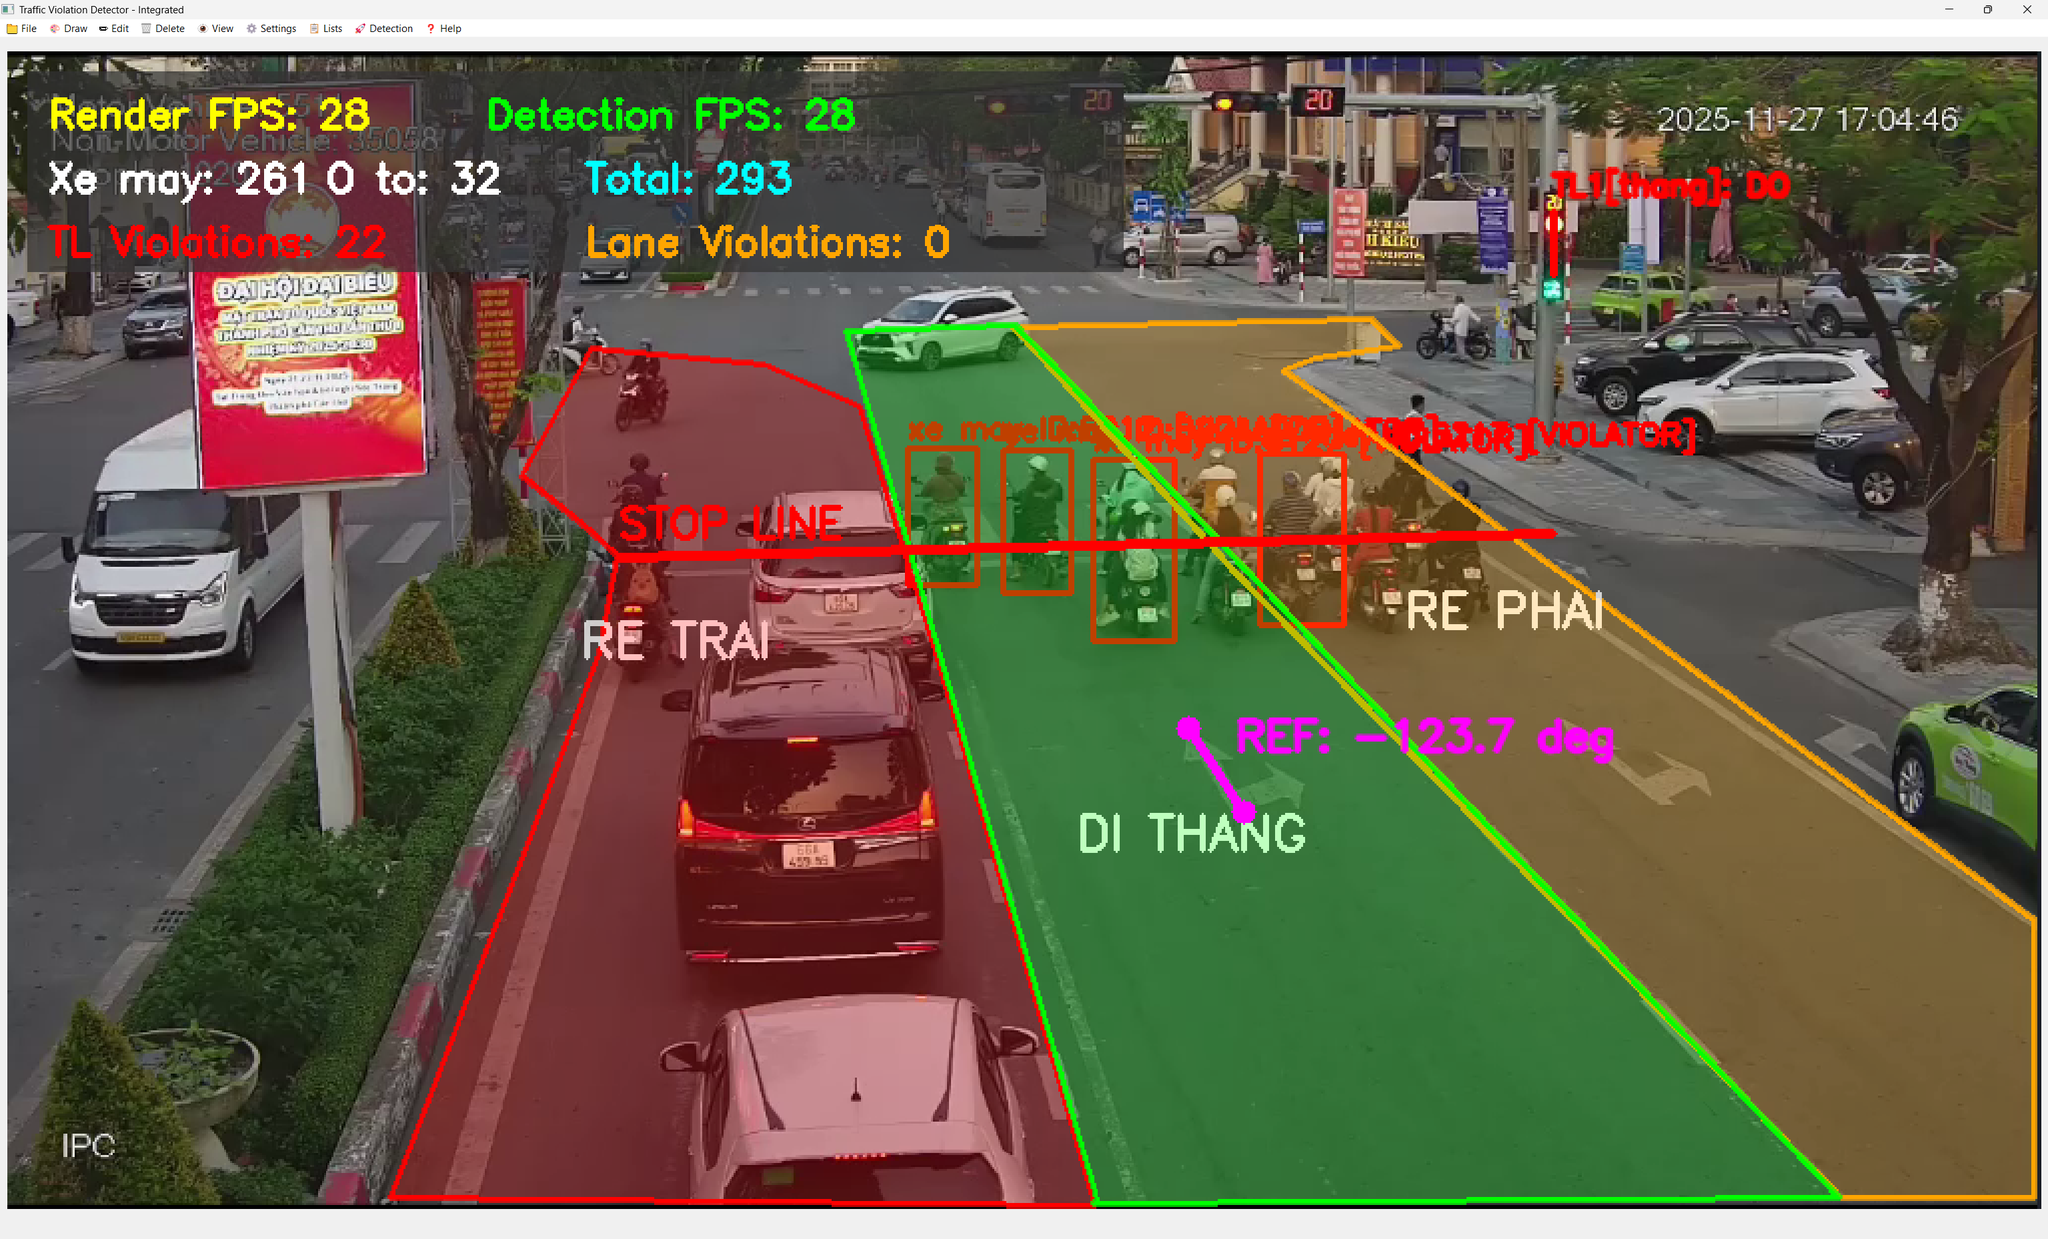
\includegraphics[width=0.7\linewidth]{Figures/inference1.png}

    \vspace{0.3cm}
    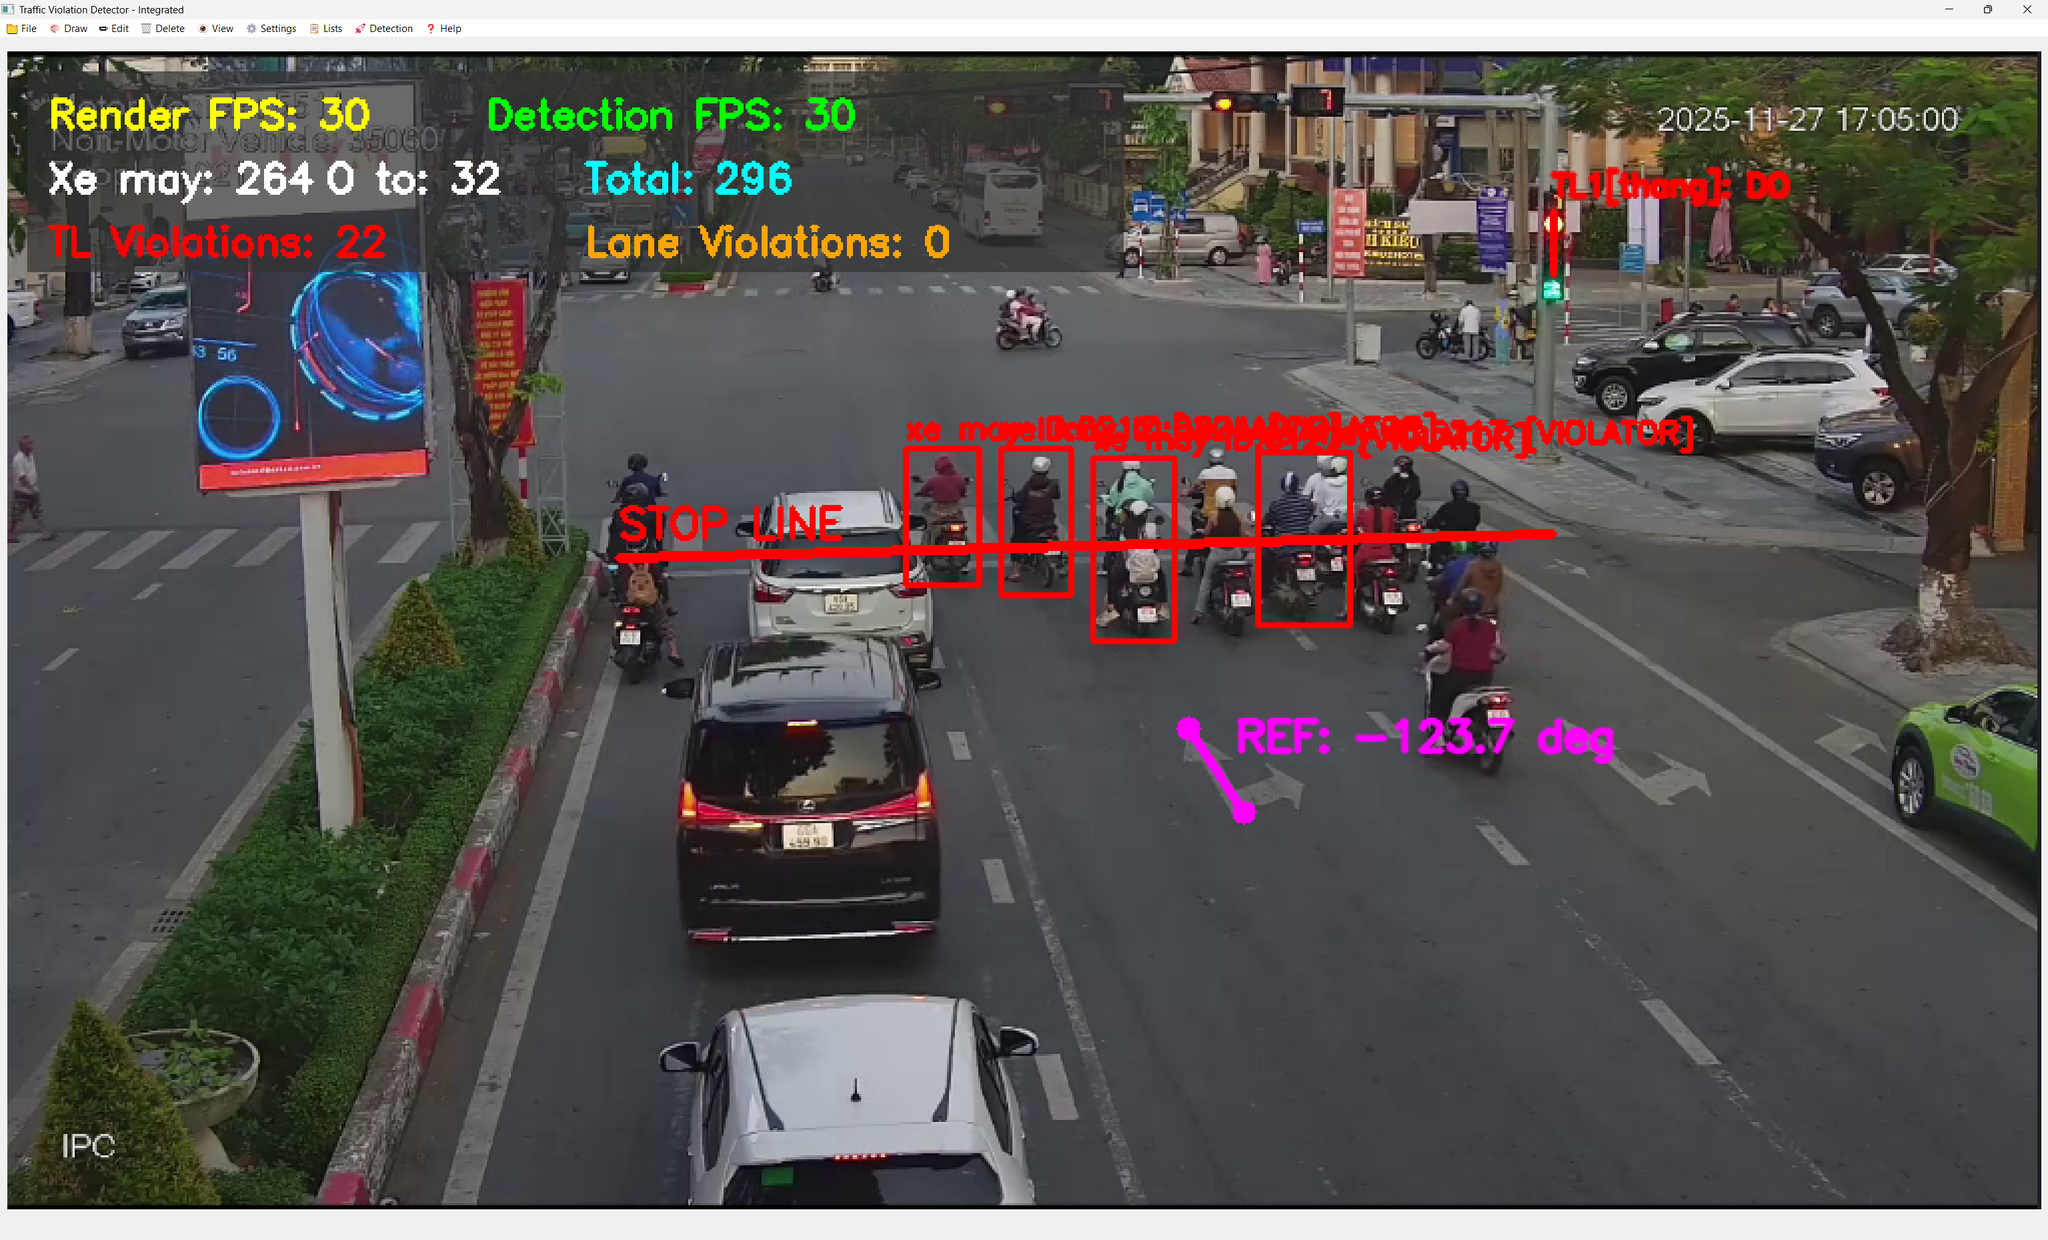
\includegraphics[width=0.7\linewidth]{Figures/inference2.png}

    \vspace{0.3cm}
    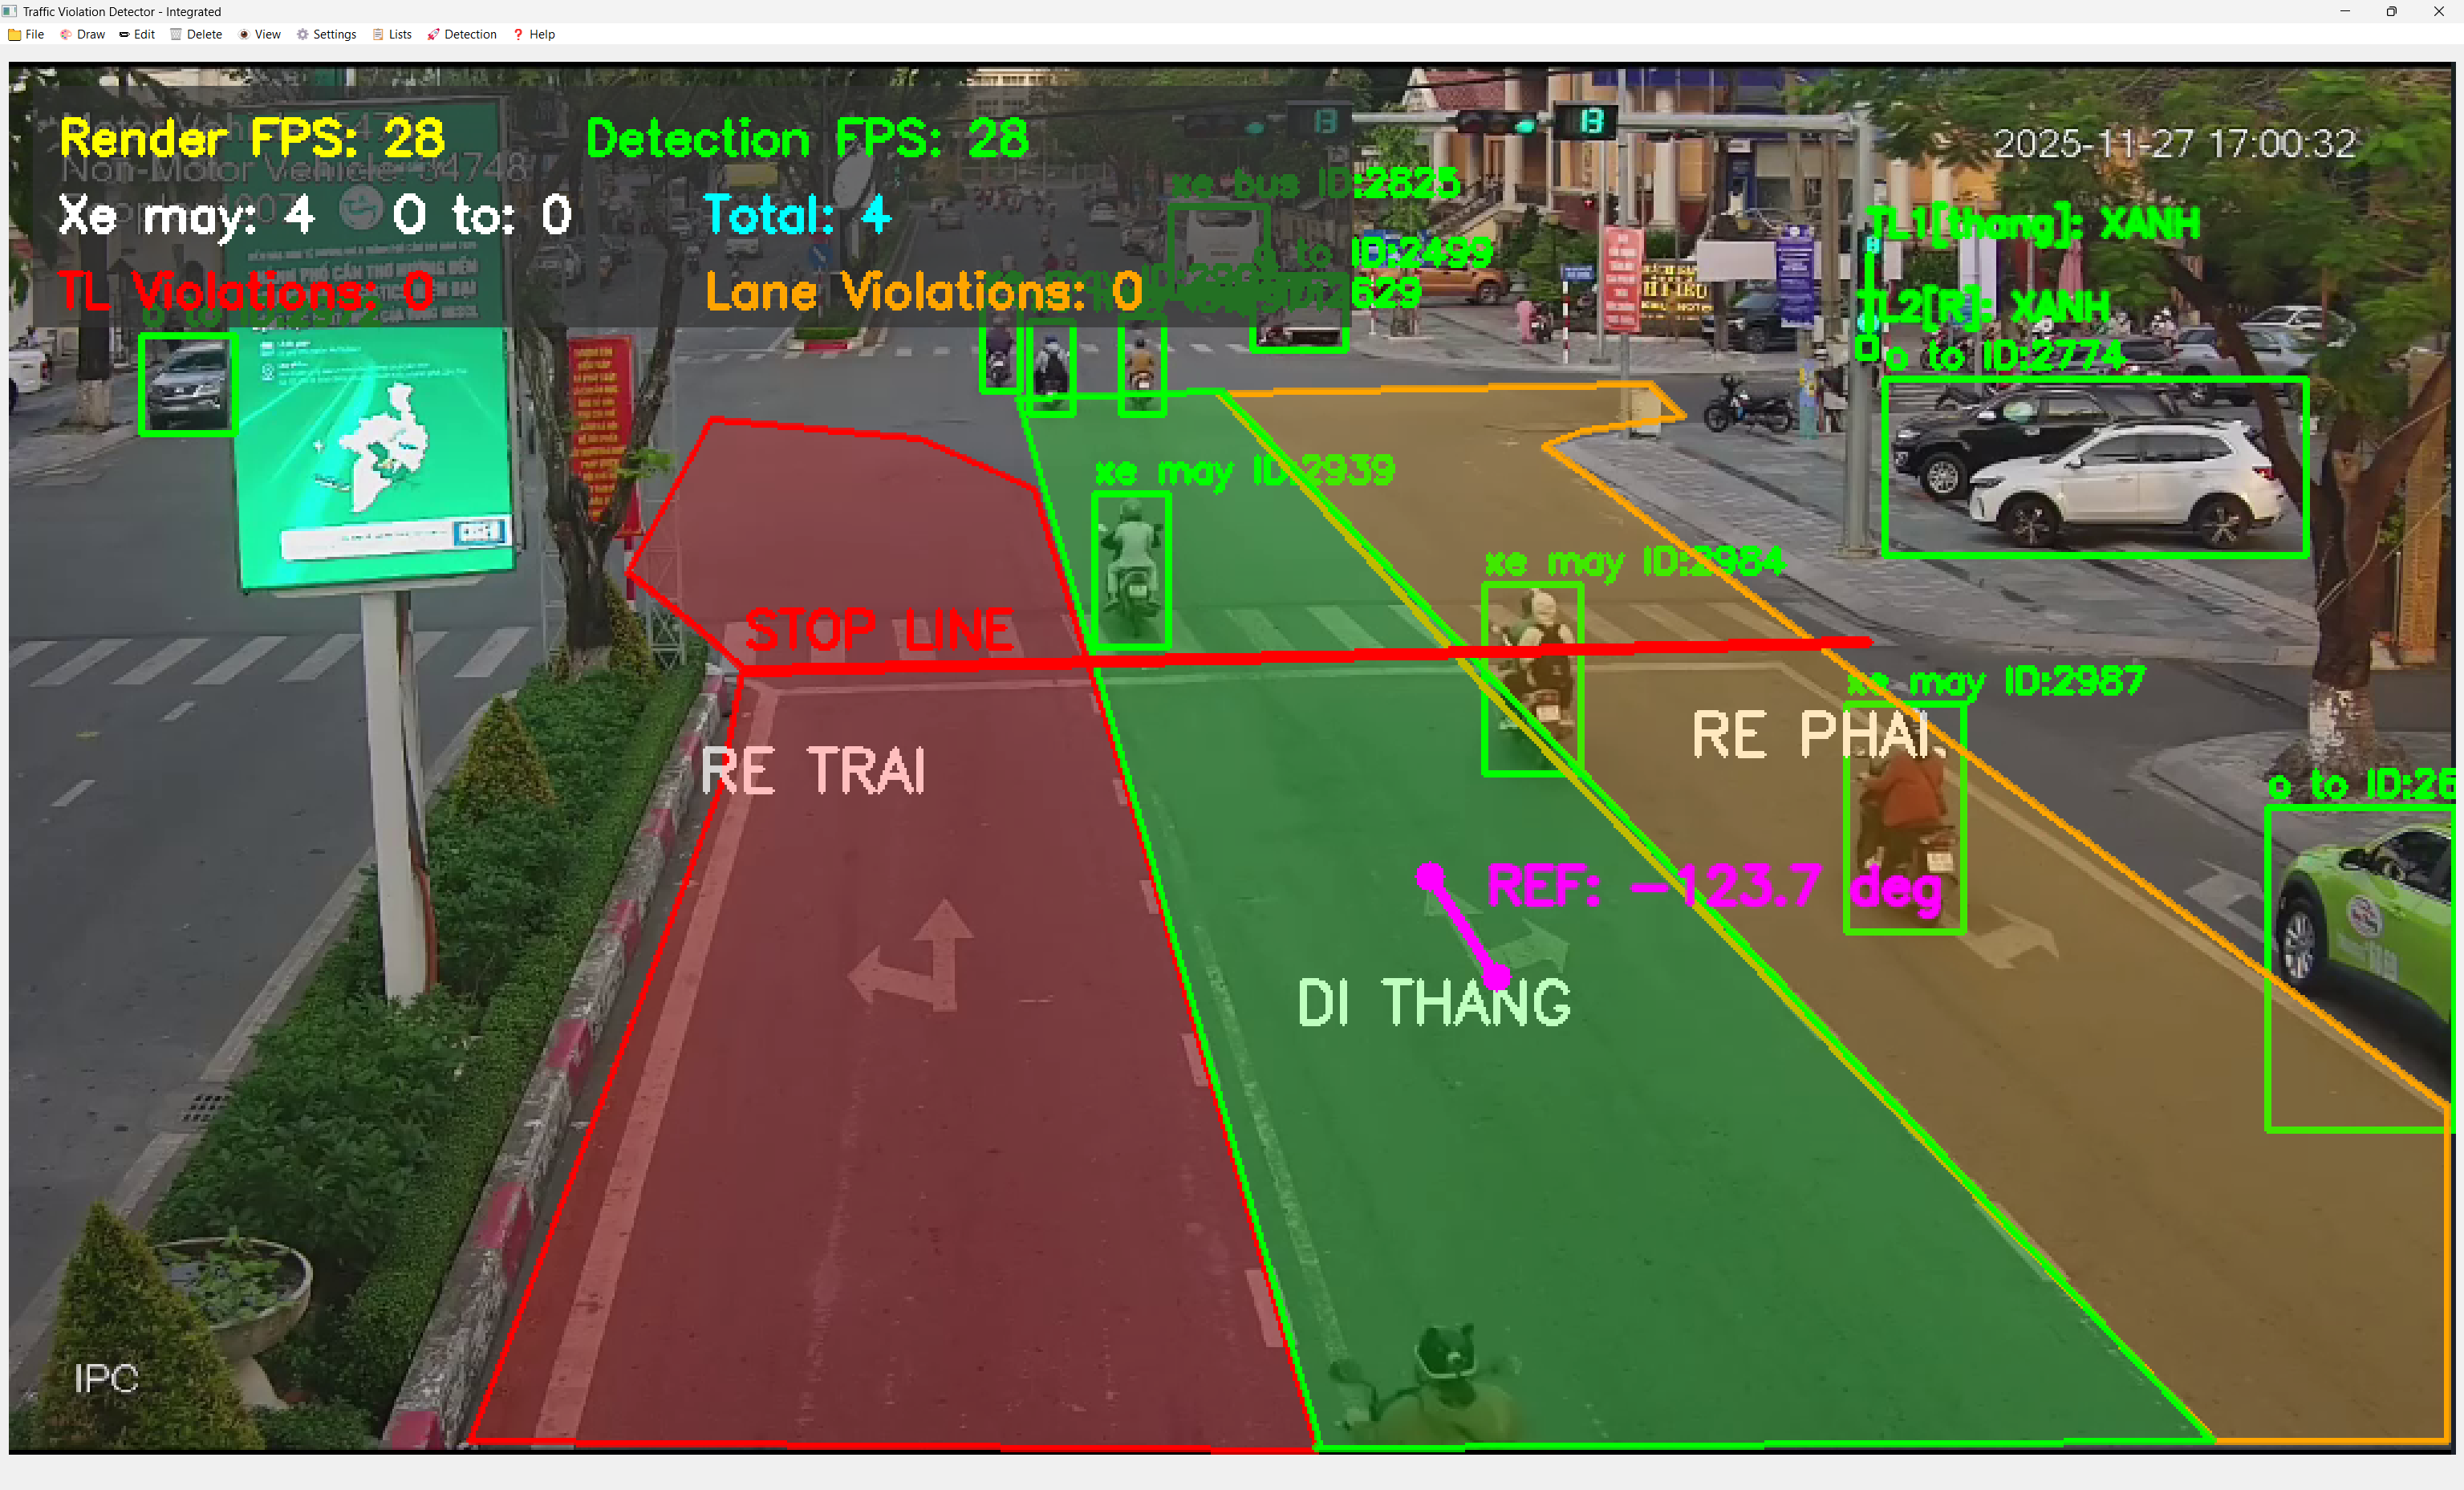
\includegraphics[width=0.7\linewidth]{Figures/Screenshot 2025-11-29 225155.png}
    \caption{Minh hoạ các phương tiện với tín hiệu đèn giao thông}
    \label{fig:inference_traffic}
\end{figure}

\begin{figure}[H]
    \centering
    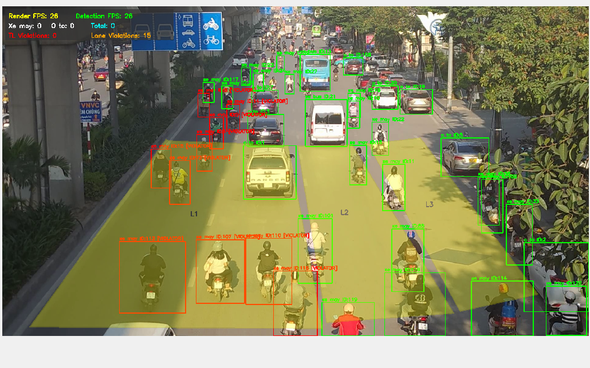
\includegraphics[width=0.7\linewidth]{Figures/inference3.png}
    \caption{Minh hoạ xe vi phạm làn đường}
    \label{fig:inference_lane}
\end{figure}

%============================================================
% PHẦN 7: THÁCH THỨC VÀ HẠN CHẾ
%============================================================
\section{Thách thức và Hạn chế}

\subsection{Các trường hợp khó với phát hiện phương tiện}
\begin{enumerate}
    \item \textbf{Nhầm lẫn xe đạp - xe máy:} Tỷ lệ nhầm lẫn 18\% do hình dáng tương đồng
    \item \textbf{Xe bị che khuất nặng:} Khó phát hiện khi chỉ nhìn thấy một phần nhỏ
    \item \textbf{Điều kiện ánh sáng yếu:} Hiệu suất giảm vào ban đêm hoặc khi có sương mù
\end{enumerate}

\subsection{Các trường hợp khó với nhận diện biển số}
\begin{enumerate}
    \item \textbf{Biển số bẩn/mờ:} CLAHE giúp cải thiện nhưng vẫn hạn chế với biển quá bẩn
    \item \textbf{Góc nghiêng lớn:} Biển số bị perspective distortion làm giảm độ chính xác OCR
    \item \textbf{Ánh sáng ban đêm:} Phản sáng từ đèn flash có thể làm mất chi tiết
    \item \textbf{Biển số nhỏ/xa:} Độ phân giải thấp khiến OCR khó nhận diện
\end{enumerate}

\subsection{Hạn chế hiện tại của hệ thống}
\begin{itemize}
    \item Tốc độ giảm khi có nhiều xe trong frame (do OCR từng biển)
    \item Chưa có cơ chế auto-retry khi OCR confidence thấp
    \item Yêu cầu cấu hình ROI thủ công cho mỗi camera mới
    \item Chưa hỗ trợ tracking xuyên camera (cross-camera tracking)
\end{itemize}

%============================================================
% PHẦN 8: TỔNG KẾT THỰC NGHIỆM
%============================================================
\section{Tổng kết thực nghiệm}




Hệ thống đã đạt được các kết quả đáng chú ý:
\begin{itemize}
    \item \textbf{Phát hiện phương tiện:} mAP@50 đạt 86.1\%, đủ tốt cho giám sát giao thông thực tế
    \item \textbf{Tracking:} ByteTrack giữ được ID ổn định với tỷ lệ ID switches < 5\%
    \item \textbf{Phát hiện vi phạm:} Logic hoạt động chính xác 100\% trên các test case, với tỷ lệ false positive rất thấp (< 2\%)
    \item \textbf{Tốc độ:} Đạt 5--20 FPS tùy phương pháp ALPR
\end{itemize}

